\documentclass[a4paper,11pt]{book}
%\documentclass[a4paper,twoside,11pt,titlepage]{book}
\usepackage{listings}
\usepackage[utf8]{inputenc}
\usepackage[spanish]{babel}

\usepackage{pdfpages}
\usepackage[square,numbers]{natbib}
\usepackage[nottoc]{tocbibind}
\usepackage{dcolumn}
\usepackage{float}
%\usepackage{doxygen/doxygen}
\usepackage{url}
\usepackage{colortbl,longtable}
\usepackage[stable]{footmisc}
%\usepackage{index}
%\usepackage[chapter]{algorithm}
\RequirePackage{verbatim}
%\RequirePackage[Glenn]{fncychap}
\usepackage{fancyhdr}
\usepackage{graphicx}
\usepackage{afterpage}
\usepackage{longtable}
\usepackage[pdfborder={000}]{hyperref} %referencia
\usepackage[nottoc]{tocbibind}
\usepackage{booktabs}
\usepackage{multirow}
\usepackage[table,xcdraw]{}
%\usepackage[style=list, number=none]{glossary} %
%\usepackage{titlesec}
%\usepackage{pailatino}
%\usepackage[table,xcdraw]{xcolor}
%\decimalpoint


% ********************************************************************
% Re-usable information
% ********************************************************************
\newcolumntype{.}{D{.}{\esperiod}{-1}}
\makeatletter
\makeatother


\newcommand{\myTitle}{Trabajo Fin de Máster\xspace}
\newcommand{\myDegree}{Máster Universitario de Investigación en Ingeniería de Software y Sistemas Informáticos\xspace}
\newcommand{\myName}{César Hugo Bárzano Cruz\xspace}
\newcommand{\myProf}{Rubén Heradio\xspace}
\newcommand{\myFaculty}{ Universidad Nacional de Educación a Distancia\xspace}
\newcommand{\myFacultyShort}{UNED-Facultad de informática\xspace}
\newcommand{\myDepartment}{\xspace}
\newcommand{\myUni}{\protect{ Universidad Nacional de Educación a Distancia}\xspace}
\newcommand{\myLocation}{Madrid\xspace}
\newcommand{\myTime}{\today\xspace}
\newcommand{\myVersion}{Versión 0.1\xspace}


\hypersetup{
pdfauthor = {\myName hugobarzano@gmail.com},
pdftitle = {\myTitle},
pdfsubject = {},
pdfkeywords = {},
pdfcreator = {LaTeX con el paquete TEXmaker},
pdfproducer = {pdflatex}
}

%\hyphenation{}




%\makeindex
%\usepackage[style=long, cols=2,border=plain,toc=true,number=none]{glossary}
% \makeglossary

% Definición de comandos que me son tiles:
%\renewcommand{\indexname}{Índice alfabético}
%\renewcommand{\glossaryname}{Glosario}

\pagestyle{fancy}
\fancyhf{}
\fancyhead[LO]{\leftmark}
\fancyhead[RE]{\rightmark}
\fancyhead[RO,LE]{\textbf{\thepage}}
\renewcommand{\chaptermark}[1]{\markboth{\textbf{#1}}{}}
\renewcommand{\sectionmark}[1]{\markright{\textbf{\thesection. #1}}}

\setlength{\headheight}{1.5\headheight}


\usepackage{bera}% optional: just to have a nice mono-spaced font
\usepackage{listings}
%\usepackage{xcolor}


\colorlet{punct}{red!60!black}
\definecolor{background}{HTML}{EEEEEE}
\definecolor{delim}{RGB}{20,105,176}
\colorlet{numb}{magenta!60!black}

\lstdefinelanguage{json}{
    basicstyle=\normalfont\ttfamily,
    numbers=left,
    numberstyle=\scriptsize,
    stepnumber=1,
    numbersep=8pt,
    showstringspaces=false,
    breaklines=true,
    frame=lines,
    backgroundcolor=\color{background},
    literate=
     *{0}{{{\color{numb}0}}}{1}
      {1}{{{\color{numb}1}}}{1}
      {2}{{{\color{numb}2}}}{1}
      {3}{{{\color{numb}3}}}{1}
      {4}{{{\color{numb}4}}}{1}
      {5}{{{\color{numb}5}}}{1}
      {6}{{{\color{numb}6}}}{1}
      {7}{{{\color{numb}7}}}{1}
      {8}{{{\color{numb}8}}}{1}
      {9}{{{\color{numb}9}}}{1}
      {:}{{{\color{punct}{:}}}}{1}
      {,}{{{\color{punct}{,}}}}{1}
      {\{}{{{\color{delim}{\{}}}}{1}
      {\}}{{{\color{delim}{\}}}}}{1}
      {[}{{{\color{delim}{[}}}}{1}
      {]}{{{\color{delim}{]}}}}{1},
}


\newcommand{\HRule}{\rule{\linewidth}{0.5mm}}
%Definimos los tipos teorema, ejemplo y definición podremos usar estos tipos
%simplemente poniendo \begin{teorema} \end{teorema} ...
\newtheorem{teorema}{Teorema}[chapter]
\newtheorem{ejemplo}{Ejemplo}[chapter]
\newtheorem{definicion}{Definición}[chapter]

\definecolor{gray97}{gray}{.97}
\definecolor{gray75}{gray}{.75}
\definecolor{gray45}{gray}{.45}
\definecolor{gray30}{gray}{.94}

\lstset{ frame=Ltb,
     framerule=0.5pt,
     aboveskip=0.5cm,
     framextopmargin=3pt,
     framexbottommargin=3pt,
     framexleftmargin=0.1cm,
     framesep=0pt,
     rulesep=.4pt,
     backgroundcolor=\color{gray97},
     rulesepcolor=\color{black},
     %
     stringstyle=\ttfamily,
     showstringspaces = false,
     basicstyle=\scriptsize\ttfamily,
     commentstyle=\color{gray45},
     keywordstyle=\bfseries,
     %
     numbers=left,
     numbersep=6pt,
     numberstyle=\tiny,
     numberfirstline = false,
     breaklines=true,
   }

% minimizar fragmentado de listados
\lstnewenvironment{listing}[1][]
   {\lstset{#1}\pagebreak[0]}{\pagebreak[0]}

\lstdefinestyle{CodigoC}
   {
	basicstyle=\scriptsize,
	frame=single,
	language=C,
	numbers=left
   }
\lstdefinestyle{CodigoC++}
   {
	basicstyle=\small,
	frame=single,
	backgroundcolor=\color{gray30},
	language=C++,
	numbers=left
   }


\lstdefinestyle{Consola}
   {basicstyle=\scriptsize\bf\ttfamily,
    backgroundcolor=\color{gray30},
    frame=single,
    numbers=none
   }


\newcommand{\bigrule}{\titlerule[0.5mm]}
\usepackage{enumitem}


%Para conseguir que en las páginas en blanco no ponga cabeceras
\makeatletter
\def\clearpage{%
  \ifvmode
    \ifnum \@dbltopnum =\m@ne
      \ifdim \pagetotal <\topskip
        \hbox{}
      \fi
    \fi
  \fi
  \newpage
  \thispagestyle{empty}
  \write\m@ne{}
  \vbox{}
  \penalty -\@Mi
}
\makeatother


\begin{document}
\begin{titlepage}
 
 
\newlength{\centeroffset}
\setlength{\centeroffset}{-0.5\oddsidemargin}
\addtolength{\centeroffset}{0.5\evensidemargin}
\thispagestyle{empty}

\noindent\hspace*{\centeroffset}\begin{minipage}{\textwidth}

\centering

\includegraphics[width=0.7\textwidth]{imagenes/Logo-uned.jpg}\\[1.1cm]


{\Huge\bfseries Máster Universitario de Investigación en Ingeniería De Software Y Sistemas Informáticos\\
}
\noindent\rule[-1ex]{\textwidth}{3pt}\\[3.5ex]
{\large\bfseries 31105151 - Trabajo Fin de Máster}
\end{minipage}

\vspace{2.5cm}
\noindent\hspace*{\centeroffset}\begin{minipage}{\textwidth}
\centering

\textbf{Autor}\\ {César Hugo Bárzano Cruz}\\[2.5ex]
\textbf{Tutor}\\ {Rubén Heradio}\\[2.5ex]


%
\includegraphics[width=0.3\textwidth]{imagenes/Logo-master.png}\\[0.1cm]
\textsc{Generative Cloud Manager: code-runner}\\
\textsc{---}\\
2019/2020
\end{minipage}
%\addtolength{\textwidth}{\centeroffset}
%\vspace{\stretch{2}}
\end{titlepage}

\begin{titlepage}
 
 

\setlength{\centeroffset}{-0.5\oddsidemargin}
\addtolength{\centeroffset}{0.5\evensidemargin}
\thispagestyle{empty}

\noindent\hspace*{\centeroffset}\begin{minipage}{\textwidth}

\centering


{\Huge\bfseries Máster Universitario de Investigación en Ingeniería De Software Y Sistemas Informáticos\\}

\noindent\rule[-1ex]{\textwidth}{3pt}\\[3.5ex]
{\large\bfseries 31105151 - Trabajo Fin de Máster}
\textbf{Generative Cloud Manager: code-runner}\\[2.5ex]
{Consultar el tipo de trabajo: Trabajo Propuesto por Alumno}\\[2.5ex]
\end{minipage}

\vspace{2.5cm}
\noindent\hspace*{\centeroffset}\begin{minipage}{\textwidth}
\centering

\textbf{Autor}\\ {César Hugo Bárzano Cruz}\\[2.5ex]
\textbf{Tutor}\\ {Rubén Heradio}\\[2.5ex]



\includegraphics[width=0.3\textwidth]{imagenes/Logo-master.png}\\[0.1cm]
\textsc{---}\\
2019/2020
\end{minipage}

\end{titlepage}




%
\includepdf{autoriza}
%\afterpage{\null\newpage}



\vspace{2.5cm}
\noindent\hspace*{\centeroffset}\begin{minipage}{\textwidth}
\setlength{\centeroffset}{-0.5\oddsidemargin}
\addtolength{\centeroffset}{0.5\evensidemargin}
\thispagestyle{empty}
\centering

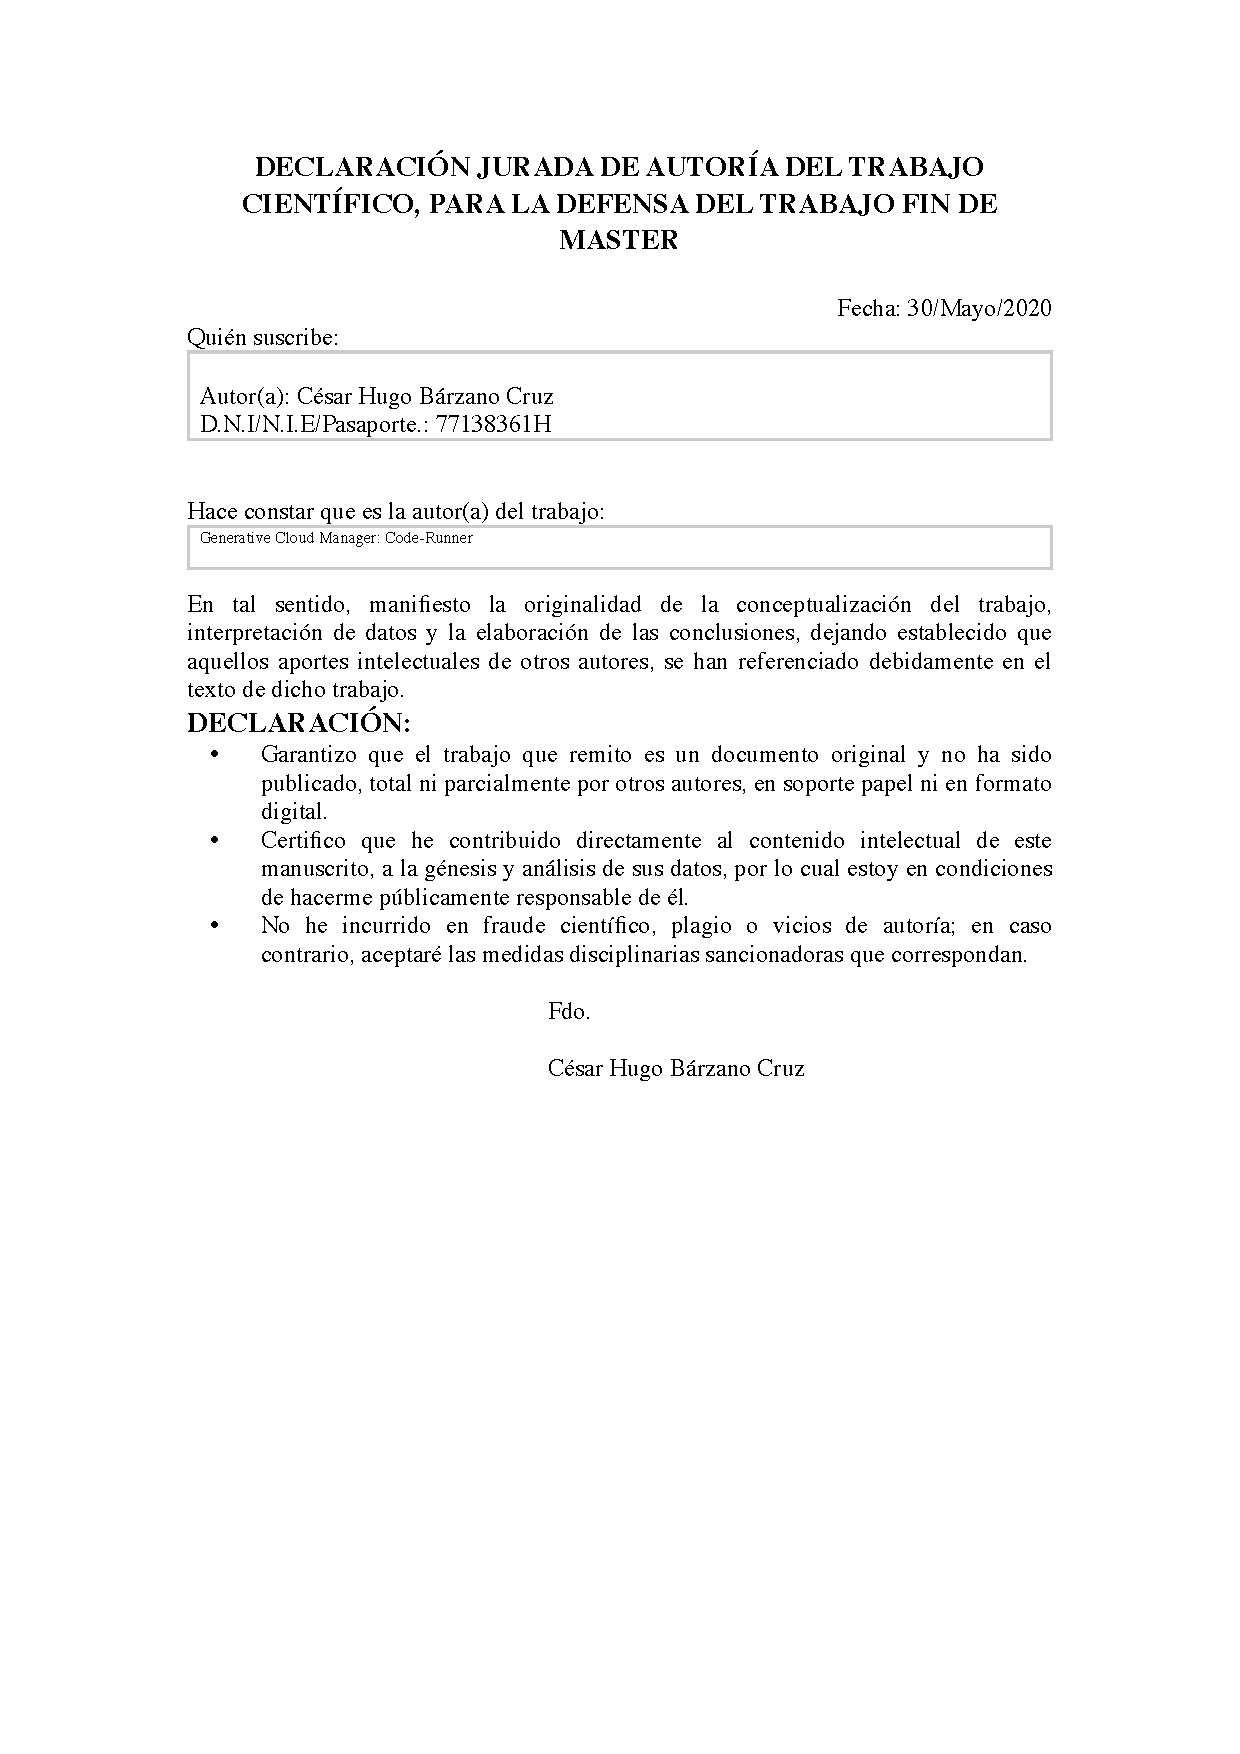
\includepdf{declara}

\afterpage{\null\newpage}
\newpage



\end{minipage}

%\vspace{2.5cm}
%\noindent\hspace*{\centeroffset}\begin{minipage}{\textwidth}
%\setlength{\centeroffset}{-0.5\oddsidemargin}
%\addtolength{\centeroffset}{0.5\evensidemargin}
%\thispagestyle{empty}
%\centering
%{\Huge\bfseries DECLARACIÓN JURADA DE AUTORÍA DEL TRABAJO CIENTÍFICO, PARA LA DEFENSA DEL TRABAJO FIN DE MASTER
%\\}
%\textbf{Quien suscribe:}\\[4.5ex]
%\textbf{Autor(a)}\\ {César Hugo Bárzano Cruz}\\[2.5ex]
%\textbf{D.N.I/N.I.E/Pasaporte.:}\\ {77138361H}\\[2.5ex]
%
%\textbf{Hace constar que es la autor(a) del trabajo:}\\ {Generative Cloud Manager: Code-Runner}\\[2.5ex]
%\textbf{Fecha}\\ {30 de Mayo de 2020}\\[2.5ex]
%
%En tal sentido, manifiesto la originalidad de la conceptualización del trabajo, interpretación de datos y la elaboración de las conclusiones, dejando establecido que aquellos aportes intelectuales de otros autores, se han referenciado debidamente en el texto de dicho trabajo.
%
%\textbf{DECLARACIÓN:}
%
%\begin{itemize}
%\item Garantizo que el trabajo que remito es un documento original y no ha sido publicado, total ni parcialmente por otros autores, en soporte papel ni en formato digital.
%\item Certifico que he contribuido directamente al contenido intelectual de este manuscrito, a la génesis y análisis de sus datos, por lo cual estoy en condiciones de hacerme públicamente responsable de él.
%\item No he incurrido en fraude científico, plagio o vicios de autoría; en caso contrario, aceptaré las medidas disciplinarias sancionadoras que correspondan
%\end{itemize}
%
%\textbf{Fdo.}\\ { César Hugo Bárzano Cruz}\\[2.5ex]
%
%\afterpage{\null\newpage}
%\newpage
%\end{minipage}

\newpage
\vspace{2.5cm}
\noindent\hspace*{\centeroffset}\begin{minipage}{\textwidth}
\setlength{\centeroffset}{-0.5\oddsidemargin}
\addtolength{\centeroffset}{0.5\evensidemargin}
\thispagestyle{empty}
\centering


\includepdf{autoriza-firmado}

\afterpage{\null\newpage}
\newpage



\end{minipage}
\newpage

\vspace{0.7cm}
\noindent{\textbf{Resumen}}\\


Este proyecto demuestra como el uso de conceptos ligados a la  Programación Generativa y la integración de diversos servicios web pueden utilizarse de manera conjunta para sintetizar, generalizar y automatizar el proceso de desarrollo y operación de aplicaciones software. La lectura aquí propuesta, junto con el sistema software resultante abordan  el proceso de desarrollo de aplicaciones software mediante un enfoque generativo, con esto  se pretende proporcionar al desarrollador software de un sistema web orientado a la generación, construcción y despliegue de aplicaciones software, concretamente de aplicaciones  web o servicios de datos en la nube.
 
 En este proyecto se considera que las etapas que forman el ciclo de vida o proceso de desarrollo de aplicaciones software está altamente segmentado, por lo que presenta una solución generativa y automatizada al proceso de desarrollo software. Con este proyecto no se pretende desprestigiar a los procesos de desarrollo software tradicionales, lo que intenta es demostrar como la unificación de los conceptos comunes entre aplicaciones web de diversa naturaleza así como la síntesis y  automatización genérica de las etapas básicas de producción software pueden dar lugar a soluciones funcionales ahorrando al desarrollador numerosas horas de trabajo. De igual forma, el sistema resultante  puede ser aprovechado por el desarrollador inexperto como punto de partida en su aprendizaje de las denominadas tecnologías de la información.
 
 
Este proyecto pone de manifiesto que ante la gran diversidad de tecnologías y soluciones ofrecidas por la Cloud Computing  existen definiciones, conceptos y  etapas básicas que son  comunes  y transversales  a todas ellas, independientemente de su naturaleza, dominio y propósito. Este proyecto sintetiza el proceso de desarrollo software en 3 etapas fundamentales: 

\begin{enumerate}
\item \textbf{ Code Generation. }  Etapa inicial donde se sintetiza el proceso de desarrollo software, es decir, se produce el código necesario para la solución especificada por el desarrollador. 
\item \textbf{ Artefact Generation, }  El objetivo de esta etapa es aprovechar el código fuente generado en la etapa Code Generation para producir un artefacto auto-contenido junto con la configuración necesaria para su ejecución en un entorno virtual. 
\item \textbf{ Deploy Generation. } En esta etapa se aprovecha el producto de la etapa Artefact Generation para disponibilizar la solución en Internet. 
\end{enumerate}
 

En los siguientes capítulos se profundiza en estas ideas, detallando cuales son los objetivos de alto nivel o casos de uso que se esperan del sistema. Se describirá el problema planteado y se analizará en detalle la solución alcanzada.\\ \\

\noindent{\textbf{Palabras Clave}: Cloud Computing, Programación Generativa, Desarrollo Software, Código Fuente, Automatización, Integración, Despliegue, Aplicaciones, Servicios, Contenedores.}\\

\afterpage{\null\newpage}
\newpage


\newpage

\vspace{0.7cm}
\noindent{\textbf{Abstract}}\\


This project shows how using concepts of  Generative Programming and the integration of web services can work toogether to synthesize, generalize and automate the process of  software development and software operation. This proyecct  addresses the process of developing software applications through a generative approach, with the target of provide a web system oriented to software generation, artefact construction and applicatiioons deployment, specifically from web applications or cloud data services.

 
This project considers that the stages of software applications developements are highly segmented, so this proyect presents a generative and automated solution to the software development. This project is not intended to discredit traditional software development but rather to show how the unification of common concepts among web applications kinds as well as the generic synthesis and automation of the basic stages of software production can lead to functional solutions saving developers from larges amounts of work. In the same line, the system can be used by the juniors developers as a starting point in their learning path of the information technologies.
 
 
This project shows that given the great diversity of technologies and solutions offered by Cloud Computing, there are definitions, concepts and basic stages that are common and transversal to all of them, regardless of their nature, domain or purpose. This project synthesizes the software development process in 3 fundamental stages:

\begin{enumerate}
\item \textbf{ Code Generation. }  Initial stage where the software development process is synthesized. Source code necessary for the solution specified by the developer is produced.

\item \textbf{ Artefact Generation }  The goal of this stage is to use the source code generated in the Code Generation stage to produce a self-contained artifact along with the necessary setup for its execution in a virtual environment.

\item \textbf{ Deploy Generation } Final stage where the product of the Artefact Generation stage is used to run the solution and make it available to developers over Internet.
\end{enumerate}
 

The following chapters delve into these ideas, describing project objectives and use cases expected from the system. The problem will be officially presented and the solution reached will be analyzed in detail.

\noindent{\textbf{Keywords}: Cloud Computing, Generative programming, Software Development, Source Code, Automation, Integration, Deployment, Applications, Services, Docker.}\\

\afterpage{\null\newpage}
\newpage
\newpage

\vspace{0.7cm}
\noindent{\textbf{Agradecimientos}}\\


Al Amor de mi vida, donde quiera que esté. 
%\frontmatter
\tableofcontents
\listoffigures
\bibliographystyle{elsarticle-num}

\chapter{Introducción}

\section{Motivación}

Este proyecto surge con la motivación de demostrar como la programación generativa y  la integración de diversos servicios web pueden utilizarse de manera conjunta para generalizar y automatizar el proceso de desarrollo y operaciones de aplicaciones web o servicios cloud.

Este proyecto aborda el proceso de desarrollo de aplicaciones web desde un punto de vista generativo.  Con esta iniciativa se pretende acuñar el lema \textbf{From Spec to Cloud} es decir, dada una definición de aplicación especifica de dominio, construir un sistema que generalice este tipo de soluciones y sea capaz de materializarlas en sistemas de información disponibles a través de Internet. De igual forma, con este proyecto se pretende dotar a los desarrolladores o clientes de un sistema que les ayude a comprender y adquirir conocimientos relativos a las tecnologías de la información y al ciclo de vida de las aplicaciones software.

A continuación se van a definir los objetivos propuestos a alcanzar siguiendo esta motivación.

\section{Objetivos}

El principal objetivo de este proyecto es el de sintetizar y automatizar el proceso de desarrollo y operación de software, concrétamente el de aplicaciones web o servicios de datos en la nube mediante un enfoque generativo. Dicha síntesis consiste en generalizar la naturaleza de los distintos sistemas de información que pueden ser consumidos a través de Internet en una única entidad denominada comúnmente como aplicación.

Para alcanzar el principal objetivo, este proyecto ha de identificar, modelar y automatizar las principales etapas del ciclo de vida de proyectos software, y construir un mecanismo genérico con el que producir aplicaciones. Las aplicaciones producidas por el proyecto han de ser auto-contenidas y auto-consumibles, es decir, han te contener todo lo necesario para ser ejecutadas y usadas fuera del marco de este proyecto.

Finalmente, este proyecto ha de definir e implementar un mecanismo genérico que permita consumir las aplicaciones producidas a través de Internet, cumpliendo así completamente con el principal objetivo.


De manera adicional, este proyecto tiene como objetivo presentar mejoras y automatizaciones relativas a los proceso de desarrollo software. El sistema resultante se presenta como una herramienta o ayuda para desarrolladores en la adquisición de conocimientos  en las denominadas tecnologías de la información. Tanto el código fuente de este proyecto como las aplicaciones creadas por los usuarios que utilicen el sistema se consideran  \textbf{Open Source}, es decir código abierto y disponible públicamente para quien lo necesite en el repositorio del proyecto \url{https://github.com/hugobarzano/GCM}.

\begin{itemize}
\item \textbf{OBJ-1. } Sintetizar y generar aplicaciones software de diversa naturaleza.
\item \textbf{OBJ-2. } Sintetizar y generar aplicaciones software de diversa tecnología.
\item \textbf{OBJ-3. } Generar aplicaciones auto-contenidas.
\item \textbf{OBJ-4. } Producir y publicar el código fuente de las aplicaciones.
\item \textbf{OBJ-5. } Producir y publicar paquetes o ejecutables de las aplicaciones.
\item \textbf{OBJ-6. } Disponibilizar aplicaciones a través de Internet.
\item \textbf{OBJ-7. } Analizar y Operar  aplicaciones en ejecución. 
\end{itemize}

A continuación se va a describir de manera literaria el problema planteado por este proyecto. 

\section{Problema}

Como se verá en el capítulo dedicado a los trabajos relacionados, el conjunto de soluciones que ofrece la nube es muy variado. Para cada una de las soluciones cloud, se pueden encontrar diversas implementaciones con diversas tecnologías, lo que incrementa
de manera significativa el conjunto final de productos software disponibles para ser consumidos por Internet. Este es el primer problema que intenta abordar este proyecto, ¿Como manejar la diversidad tecnológica que produce trabajar en entornos de computación
en la nube? ¿Qué solución es mas adecuada para un problema concreto de negocio? ¿Con qué tecnología implementar la solución elegida? Este proyecto aborda este problema dotando a los desarrolladores de una plataforma Open Source donde probar la tecnología que desean construir.\\

El conjunto de soluciones ofrecidas por los diversos proveedores de soluciones cloud aumenta día a día en función de las necesidades de negocio de los consumidores lo que obliga a los profesionales a estar continuamente renovando y certificando sus conocimientos. A raíz de esto han surgido muchas plataformas de aprendizaje o E-learning para que los profesionales adquieran conocimientos en las consideras tecnologías de vanguardia,  en otras palabras, tecnologías altamente demandadas por el mundo empresarial. Algunas de esta plataformas son:

\begin{itemize}
\item \href{https://linuxacademy.com/}{Linux Academy}
\item \href{https://es.coursera.org/}{Coursera}
\item \href{https://www.udemy.com}{Udemi}
\end{itemize}

Estas plataformas cuentan con diversos recursos virtuales para el aprendizaje ( videos, tutoriales, laboratorios virtuales, ejercicios, test) pero ninguna de ellas materializa el tipo de software que el desarrollador desea aprender en una aplicación o servicio consumible a través de Internet siendo este uno de los objetivos a alcanzar por el proyecto aquí planteado. \\


Normalmente en los proyectos informáticos las etapas que forman el ciclo de vida del desarrollo software están altamente segmentadas y debido a esto el tiempo y recursos necesarios para diseñar, implementar y desplegar un producto software es elevado.  Este proyecto intenta mejorar esto dando un enfoque reducido, generativo y automatizado para la especificación, producción y despliegue de software en entornos de computación en la nube.  

A continuación, se va a describir la solución alcanzada por este proyecto. 

\section{Solución}

Este proyecto muestra como el uso de la programación generativa y las tecnologías de la información mejoran el proceso desarrollo y despliegue software en el ámbito de las soluciones orientadas a la web 2.0. Se pretende proporcionar al desarrollador software de un sistema web orientado a la generación, construcción y despliegue de aplicaciones web o servicios de datos de diversa naturaleza partiendo de una definición especifica de dominio. Con esta solución se intenta que el desarrollador adquiera conceptos y conocimientos relativos a las tecnologías de la información y el ciclo de vida del desarrollo software.  \\

Como solución se propone realizar las siguientes síntesis o generalidades.  Por una parte, ante la gran diversidad de soluciones cloud: 

\begin{enumerate}
\item \textbf{ Aplicaciones web estáticas }
\item \textbf{ Aplicaciones web dinámicas}
\item \textbf{ Interfaces web }
\item \textbf{ Api/Rest }
\item \textbf{ Servicios de Datos }
\end{enumerate}

Se propone sintetizar todas ellas  como una única  entidad \textbf{aplicación} y  someter a esta entidad al mismo proceso o etapas independientemente de cual sea su naturaleza o dominio cumpliendo con el objetivo de dada una especificación de aplicación, producir el código fuente necesario para materializar dicha especificación en un producto software funcional. 



La entidad de propósito general \textbf{aplicación} es definida por el siguiente conjunto de recursos:    

\begin{enumerate}
\item \textbf{ Repositorio de Código Fuente. } Lugar donde habita la aplicación. 
\item \textbf{ README.} Fichero descriptivo con información relativa a  la aplicación. 
\item \textbf{ LICENCE. }Fichero descriptivo caracterizando la aplicación como Open Source. 
\item \textbf{ makefile.} Herramienta  de construcción, permite realizar operacionales básicas a nivel de proyecto software:

  \begin{enumerate}[label*=\arabic*.]
    \item make setup:  Instalación
    \item make build:  Compilación
    \item make test: Ejecución Pruebas Unitarias
   	\item make run: Ejecución
   	\item make pull: Descargar Artefacto
   	\item make push: Crear Artefacto	
  \end{enumerate}
  
  
\item \textbf{ Codigo Fuente.}Representa el software en si, contiene la lógica de la aplicación.  
\item \textbf{ Configuración.} Representa la configuración necesaria para ejecutar la aplicación. 
\item \textbf{ Documentación.} Representa la documentación o especificación de la aplicación. 
\item \textbf{ Dockerfile.} Define al artefacto necesario para ejecutar la aplicación. Dicho artefacto es una Imagen docker. 
\end{enumerate}




Por otra parte, sintetizar el proceso de desarrollo y despliegue de software de manera automatizada y generativa  este proyecto define las siguientes etapas: 

\begin{enumerate}
\item \textbf{ Code Generation }  Etapa inicial donde se sintetiza el proceso de desarrollo software, es decir se produce el código necesario para la solución especificada por el desarrollador.
\item \textbf{ Artefact Generation }  El objetivo de esta etapa es aprovechar el código fuente generado en la etapa Code Generation para producir un artefacto auto-contenido junto con la configuración necesaria para su ejecución en un entorno virtual.
\item \textbf{ Deploy Generation } En esta etapa se aprovecha el producto de la etapa Artefact Generation para disponibilizar la solución en Internet.
\end{enumerate}

Toda aplicación generada por el sistema es sometida a estas etapas, independientemente de su naturaleza, dominio o tecnología. Con ellas se consigue que dada una especificación de aplicación se genere y publique el código fuente que materializa la definición en producto software, transformando problemas especifico de dominio en soluciones generalizadas, la construcción de artefactos auto-contenidos que permita la distribución y ejecución del software generado, así como la disponibilización de  las aplicaciones en Internet para que pueda ser consumida por los usuarios del sistema. 


En los siguientes capítulos se mostraran trabajos, publicaciones y tecnologías relacionadas con el campo de estudio aquí propuesto. Con el objetivo de facilitar la comprensión del sistema software a construir, se planifica y analiza el problema  a resolver mediante ingeniería de requisitos. Tras el análisis se detalla la implementación realizada y la consecución de los objetivos propuesto mediante un caso de uso funcional.


\chapter{Trabajos Relacionados}

En las siguientes secciones se presenta a modo de introducción conceptos relativos a Programación Generativa, Cloud Computing y conceptos relacionados con el proceso de desarrollo software y el ciclo de vida de productos software, conceptos como la Integración Continua y el Despliegue Continuo. Se pretende con esto dotar al lector de un contexto o conocimiento básico para abordar el proyecto. De manera adicional se abordan tecnologías, trabajos y publicaciones relacionadas para mostrar el estado actual del arte. 


\section{Desarrollo Software}

\subsection{Ciclo de Vida del Desarrollo Software (SDLC) }

El ciclo de vida del desarrollo software es un procedimiento sistemático para construir software.  El objetivo de este procedimiento es el de garantizar la calidad y las exactitud del software a desarrollar, haciendo que cumpla con las expectativas del usuario. 
   
\subsubsection{Etapas SDLC}

\begin{enumerate}
\item  Planificación: Etapa inicial donde se define el software a implementar, determinando el alcance que se quiere lograr. Esta etapa permite discernir el presupuesto, el tiempo y los recursos necesarios para el proyecto. 
\item Ingeniería de requisitos: Etapa en la que se pone de manifiesto cuales son los requisitos que el proyecto software ha de cumplir para ser aceptado por el cliente. 
\item Diseño: Etapa que consiste en trasformas los requisitos de alto nivel solicitados por el cliente a una realidad técnica que los equipos de expertos puedan llevar a cabo. 
\item Desarrollo: Etapa en la que los desarrolladores materializan el diseño técnico en producto software. 
\item Pruebas: Etapa en la que el equipo de calidad valida y verifica que el software desarrollado cumple los requisitos esperados por el cliente. 
\item Productivización:  Etapa en la que el equipo de operaciones disponibiliza el software para que el cliente comience a utilizarlo.
\item Mantenimiento: Etapa en la que se corrigen fallos percibidos tras un uso real del software. 
\item Disposición: Etapa en la que se contempla como será la retirada del software una vez que haya alcanzado su vida útil. 
\end{enumerate}

\subsection{Desarrollo Software y Buenas Prácticas }

En esta sección se profundiza en buenas practicas relativas al desarrollo software.

\subsubsection{Integración Continua}
 
La integración continua consiste en un modelo informático orientado al desarrollo software que propone la integración de nuevas funcionalidades y la ejecución de pruebas de manera constante para así detectar posibles problemas o regresiones en el software que se está desarrollando así como mejorar su calidad de una manera automatizada. En el artículo \textbf{Continuous Integration}\cite{ci}   Martin Fowler ejemplifica este modelo mediante la implementación de una funcionalidad mediante integración continua. 

\subsubsection{Entrega Continua}

La entrega continua es un procedimiento informático que consiste en realzar entregas continuas de versiones del software que se está construyendo. Está íntimamente ligado al modelo de Integración Continua, permite a los desarrolladores liberar versiones del producto software para que sean validadas por los responsables de calidad o integradas en entornos productivos mientras continúan desarrollando nuevas funcionalidades. El objetivo de este procedimiento es el de disponer de un artefacto listo para ser probado, ejecutado y distribuido.  En este procedimiento, la automatización llega hasta el punto de generar dicho artefacto, su despliegue o distribución requiere de intervención humana. En el articulo \textbf{Continuous Delivery: Overcoming adoption challenges}\cite{cd}, se proponen diversas estrategias para adoptar procedimientos de entrega continua  en el mundo empresarial así como retos en materia de investigación propuestos a la comunidad científica. 

\subsubsection{Despliegue Continuo}

El despliegue continuo consiste en un procedimiento automatizado similar a la entrega continua con la diferencia de que en este caso el artefacto implementado es distribuido o ejecutado sobre un entorno virtual sin interacción humana, en otras palabras, es desplegado.  De esta forma los tiempos de entrega y operación de nuevas funcionalidades software se ven notablemente reducidos. En el artículo \textbf{Problems and Solutions of Continuous Deployment: A Systematic Review}\cite{cdpl} se realiza un repaso sobre numerosos artículos relativos al despliegue continuo  poniendo de manifiesto problemas o retos encontrados al intentar adoptar este procedimiento en el mundo empresarial y que  
solución se adecua mas a cada uno de los problemas presentados. 

\subsection{En este Proyecto}

Este proyecto considera que las etapas que forman parte del ciclo de vida del desarrollo software están altamente segmentadas. Es cierto que a la hora de llevar a cabo proyectos informáticos a gran escala como los encontrados en el sector espacial o energético, los cuales involucran a diversas organizaciones,  cada una de estas etapas es necesaria ya que el volumen y la dimensión de dichos proyectos así lo requieren pero en el ámbito del desarrollo software orientado a las aplicaciones modernas, estas etapas pueden ser sintetizadas y reducidas, mejorando notablemente los tiempos de desarrollo y abaratando costes.  En las últimas 2 décadas, tras la publicación del \textbf{ Agile Manifesto}\cite{agile} la industria del software ha dado un giro orientando sus procesos hacia el cambio y mejora continua en lugar de intentar evitar o contemplar errores a priori mediante un diseño extenso y una planificación estricta.  En el articulo \textbf{ A decade of agile methodologies: Towards explaining agile software developmen}\cite{decada} se recogen  diversas publicaciones relacionadas con el desarrollo ágil así como las aportaciones realizadas al campo fruto de la investigación software. 


En linea con las buenas practicas a la hora de desarrollar software presentadas en la sección anterior,  así como las ventajas que aporta las metodologías ágiles, este proyecto sintetiza el proceso de de desarrollo software mediante un enfoque generativo, materializando una especificación de usuario en código fuente funcional.  Para implementar las buenas prácticas de Integración Continua y Entrega Continua este proyecto hace uso de \textbf{Github}\cite{github} como sistema gestor de repositorios de código así como de las herramientas que ofrece. En el capitulo 4 titulado Implementación y Pruebas, sección~\ref{repo}  Repositorio de Código se profundiza en esta cuestión. 

Por otra parte, para implementar la buena práctica de Despliegue Continuo se ha decidido utilizar como tecnología de virtualización  \textbf{Docker}\cite{dk}, lo que permite aplicar el mismo tratamiento a las diversas aplicaciones generadas por el sistema, independientemente de de su naturaleza o dominio. En la sección ~\ref{infra} 
Infraestructura Virtual de las Aplicaciones se profundiza y justifica el uso de esta tecnología para cumplir con el objetivo de desplegar y disponibilizar las aplicaciones generadas a través de Internet. De manera adicional, en la sección ~\ref{mercado} Tecnología en el Mercado se repasan las principales soluciones orientadas al problema aquí planteado que ofrece tanto la comunidad Open-Source como los proveedores de soluciones en la nube.   

\section{Programación Generativa}

La programación generativa (Generative Programaing) de manera directa trata de << Escribir programas que escriban programas. >>  para aportar beneficios al ciclo de vida del desarrollo software en aspectos tales como: 

\begin{enumerate}
\item \textbf{Productividad}:  Las técnicas de programación generativa pueden ahorrar numerosas horas de codificación.  
\item \textbf{Calidad}: El código generado mantiene una calidad uniforme a lo largo de toda la linea base de código generativo.
\item \textbf{Consistencia}: El código generado mantiene uniformidad tanto en nombrado de variables como en la firma de funciones lo que facilita su posterior mejora mediante programación manual. 
\item \textbf{Abstracción}: En algunos casos, los generadores de código utilizan como entrada un modelo abstracto del sistema que van a producir. Este modelo abstracto representa las reglas de negocio de alto nivel que el sistema producido ha de cumplir y permite que el generador sea portable ya que la misma entrada puede ser aprovechada para producir código en distintos lenguajes o tecnologías. 
\end{enumerate}

Tal y como se presenta en el articulo \textbf{Generative Programming}\cite{gp} la programación generativa consiste en diseñar e implementar módulos software que pueden ser combinados para generar sistemas especializados y  optimizados en cumplir requisitos específicos de dominio. Los objetivos de la programación generativa son:

\begin{enumerate}
\item Disminuir la desviación conceptual entre el código software y los conceptos de dominio.
\item Reutilización y adaptabilidad de módulos software.
\item Simplificar la administración de muchas variantes de un componente.
\item Aumentar la eficiencia  en capacidad y en tiempo de ejecución.
\end{enumerate}

\subsection{Principios}

Para alcanzar sus objetivos, la programación generativa ha de cumplir los siguientes principios tratados en el articulo \textbf{Generative Programming and Active Libraries}\cite{gpl}

\begin{enumerate}
\item \textbf{Separation of concerns (SoC)}. La separación de preocupaciones pone de manifiesto la importancia de lidiar con los problemas de una manera atómica. Es decir, crear pequeños fragmentos de código que cumplan con una funcionalidad muy especifica e integrarlos para dar lugar al componente deseado.
\item \textbf{Parameterization of differences}.  La parametrización de componentes da la posibilidad de representar familias de componentes.
\item \textbf{Analysis and modeling of dependencies and interactions}.  Define el termino conocimiento de configuración horizontal como la dependencia que existe en el valor que toma el parámetro de un modelo, condicionado el valor de otros parámetros del mismo modelo.
\item \textbf{Separating problem space from solution space}.  Define el termino conocimiento de configuración vertical, donde se pone de manifiesto que el espacio del problema es especifico del dominio mientras que el espació de la solución ha de ser generalizado.
\item \textbf{Eliminating overhead and performing domain-specific optimizations}.  Donde se aconseja un proceso de refinamiento tras la generación estática de componentes para eliminar software no utilizado en el dominio especifico.
\end{enumerate}

\subsection{En este proyecto}

Resulta imperativo presentar como ejemplo  la produción en cadena o la produción en escala que Henry Ford aplicó en 1908 en el sector del automóvil. Este proceso de producción industrial revoluciono el mercado ya que mejoraba los tiempos de entrega, abarataba precio de producción y garantizaba un nivel de calidad similar a lo largo de toda la linea de productos fabricados. La idea de la cadena de producción se basa en que dado un diseño, por ejemplo un coche, en cada etapa de la cadena de producción  se agrega un determinado componente y que la suma de N etapas con sus correspondientes componentes dan lugar a un producto completo y funcional, en el caso de este ejemplo un Ford T. 

En linea con este concepto de producción en cadena, el cual es aplicado hoy en día en numerosos sectores, el objetivo de este proyecto es construir una cadena de producción software que sea capaz de generar y desplegar aplicaciones, para ello este proyecto se apoya en la programación generativa para sintetizar el ciclo de vida del desarrollo software, abstrayendo al usuario de los detalles internos de programación y permitiendo generar aplicaciones mediante una especificación de alto nivel. En este sistema el objetivo  de generar aplicaciones no se limita al código fuente, si no que involucra otros aspectos como creación y configuración de recursos virtuales como por ejemplo el repositorio de código donde contener el código fuente, la configuración necesaria para dotar a las aplicaciones generadas de un ciclo de integración continua para evolucionar el código generado si fuera necesario, configuración necesaria para compilar, distribuir y disponer de artefactos ejecutables, así como  la configuración y recursos virtuales necesarios para el despliegue continuo de las aplicaciones.
 
En el libro \textbf{Code Generation in Action (In Action Series)}\cite{codeg} se presentan diversos ejemplos prácticos que han sido utilizados como referente en la implementación de este sistema para cubrir aspectos tales como:

\begin{enumerate}
\item Generación de Interfaces de usuario. 
\item Generación de documentación
\item Generación de servicios web basados en capas
\item Generación de lógica de negocio. 
\end{enumerate}


El sistema aquí propuesto entra en la categoría generativa de \textbf{model driven design}, donde la especificación de alto nivel proporcionada por el usuario define el modelo de aplicación o servicio web  que se va a generar. Para el proceso generativo se ha construido un motor de plantillas capaz de producir aplicaciones de diversa naturaleza o dominio a partir del modelo de aplicación definido como entrada por el usuario.  En el libro \textbf{Code generation with templates}\cite{templates} se presenta por una parte un enfoque matemático para justificar el uso y mejora de plantillas y por otro un enfoque práctico y aplicado de como trabajar con plantillas o como definir el meta-lenguaje necesario para las plantillas.  Como trabajo previo relacionado se hace referencia al proyecto \textbf{Apigena}\cite{apigena} donde de aborda la producción de APIs-REST mediante un enfoque generativo. 

\section{Cloud Computing}

La real academia de la ingeniería, define la computación en la nube o Cloud Computing\citep{realacademia}  como: “La Utilización de las instalaciones propias de un servidor web albergadas por un proveedor de Internet para almacenar, desplegar y ejecutar aplicaciones a petición de los usuarios demandantes de las mismas.” La computación en la nube es un paradigma en el que la información se almacena de manera permanente en servidores de internet y se ofrece, a través de aplicaciones, como servicio. El Cloud Computing es un nuevo modelo de prestación de servicios\cite{magazine} de negocio y tecnología, pagando únicamente por el consumo efectuado. Este modelo de negocio ha conseguido un lugar importante en el mercado y en la computación  por lo que se considera  interesante hacer una introducción con el objetivo de que el lector tenga un mayor grado de comprensión ya que la computación en la nube juega un papel fundamental en la resolución  del problema planteado.

La nube  o el cloud computing  puede definirse  como el conjunto de tecnologías que permiten acceder a servicios información a través de Internet, es decir, sin necesidad de instalar programas software, el usuario puede acceder a estos servicios mediante Internet. No hay que entender a la nube como una entidad física, sino como una red de servidores distribuidos en todo el mundo, que inter-conectados entre si funcionan como un único ecosistema.  El paradigma que presenta la nube se basa en que en lugar de acceder a archivos y datos desde un equipo personal o local, se accede a ellos en línea desde cualquier dispositivo conectado a Internet. La siguiente imagen muestra los beneficios de la computación en la nube:

\begin{figure}[H]
\centering
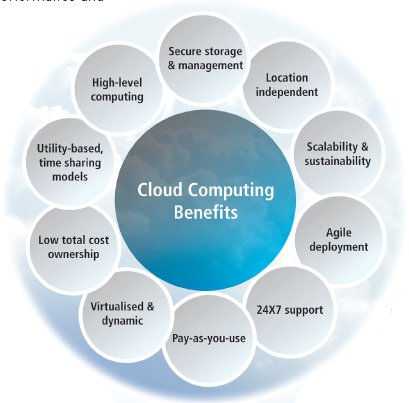
\includegraphics[scale=0.5]{imagenes/beneficiosCC.jpg}
\caption{ Beneficios Cloud Computing\cite{beneficios} }
\end{figure}


\subsection{Tipos de Nube}

La nube puede clasificarse en distintos modelos en función del tipo de solución que quiera cubrir:

\subsubsection{Nube Pública}

Las nubes públicas son propiedad de los proveedores de servicio, es decir, hardware, software y todos los componentes necesarios para la infraestructura virtual subyacente son propiedad del proveedor de servicio cuya tarea es administrarlos. El consumidor accede y administra los recursos que va a consumir desde un explorador web.  Algunos ejemplos de proveedores de nube pública son GoogleCloud\cite{gcp} , Amazon Web Services\cite{aws} o Microsoft Azure\cite{azure}

\subsubsection{Nube Privada}
Las nubes privadas se caracterizan por que sus servicios e infraestructura subyacente se mantiene en una red privada, utilizados exclusivamente por una empresa u organización. Por ejemplo, una nube privada puede encontrarse físicamente en el centro de datos de una compañía o de un banco.

\subsubsection{Nube Híbrida}

Las nubes híbridas se caracterizan por combinar los modelos de nube pública y nube privada. La nubes híbridas inter-conectan ambos modelos con el objetivo de compartir datos y aplicaciones aportando mayor flexibilidad y opciones de desarrollo, optimizando el uso de la infraestructura subyacente y la seguridad.


\subsection{Tipos de Servicios en la Nube}

La computación en la nube permite la integración de servicios en Red a nivel mundial y además contribuye al uso eficiente de la energía aunque la centralización de las aplicaciones y el almacenamiento de los datos origina una interdependencia con los proveedores de servicios. La disponibilidad de estos servicios necesita de conexión a Internet.  En el articulo \textbf{Comparison Among Cloud Technologies and Cloud Performance}\cite{cloudtech} se revisan las distintas tecnologías que configuran la nube comparando distintas herramientas para trabajar con este tipo de servicios.

Los servicios proporcionados por la nube pueden clasificarse en las siguientes categorías:

\begin{figure}[H]
\centering
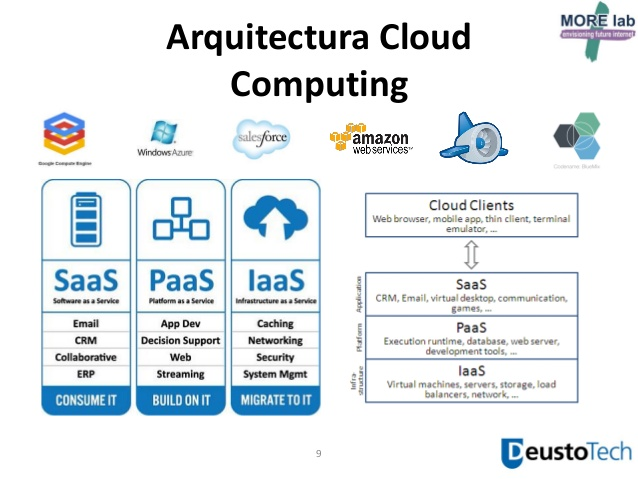
\includegraphics[scale=0.5]{imagenes/arquitecturaCC.jpg}
\caption{ Arquitectura Cloud Computing\cite{arquitecturaCC} }
\end{figure}

\subsubsection{Software como servicio (SaaS)}\label{secsaas}

El Software como Servicio\cite{saas} (SaaS, Software as a Service) ofrece el consumo de una gran variedad de aplicaciones o servicios proporcionadas por los proveedores del servicio y que se ejecutan en la infraestructura de la nube. Las aplicaciones en la nube son accesibles por distintos dispositivos del cliente a través de una interfaz sencilla, como por ejemplo un navegador web. El cliente no gestiona la infraestructura del servicio, que incluye la red de comunicaciones, los servidores, los sistemas operativos y el almacenamiento, simplemente utiliza el servicio como es el caso de este proyecto.

\subsubsection{Plataforma como servicio (PaaS)}\label{secpaas}

La Plataforma como Servicio\cite{paas} (PaaS, Platform as a Service) es una categoría de servicios cloud que proporciona un entorno a los desarrolladores crear aplicaciones y servicios que funcionen a través de internet. Los servicios PaaS se alojan en la nube, y los usuarios pueden acceder a ellos a través de un navegador web. Este tipo de servicios consisten en funcionalidades pre-configuradas a las que los clientes puedan suscribirse, eligiendo las características que deseen integrar en función de sus necesidades. Algunas de las funcionalidades PaaS son:

\begin{enumerate}
\item Sistema operativo.
\item Entorno de scripting de servidor.
\item Sistema de gestión de base de datos.
\item Software de servidor.
\item Soporte técnico.
\item Almacenamiento.
\item Acceso a la red.
\item Herramientas de diseño y desarrollo.
\item Hosting.
\end{enumerate}

\subsubsection{Infraestructura como servicio (IaaS)}

La Infraestructura como Servicio\cite{iaas} (IaaS, Infrastructure as a Service) es un servicio cloud, que proporciona acceso a recursos informáticos situados en un entorno virtualizado, a través de una conexión pública. Los recursos informáticos ofrecidos  son básicamente infraestructura de procesamiento. Físicamente, el repertorio de recursos hardware disponibles procede de multitud de servidores y redes, generalmente distribuidos entre numerosos centros de datos, de cuyo mantenimiento se encarga el proveedor del servicio cloud. El cliente, por su parte, obtiene acceso a los componentes virtualizados para construir con ellos su propia plataforma informática.

Estas son algunas de las ventajas o características de una implementación basada en el modelo de Infraestructura como Servicio:

\begin{enumerate}
\item Escalabilidad.
\item Sin necesidad de invertir en hardware.
\item Independencia de la localización.
\item Seguridad física en los centros de datos.
\end{enumerate}

\subsection{Tecnología en el Mercado}\label{mercado}

Actualmente en el mercado existen soluciones cloud que ofrecen parte de la funcionalidad que este proyecto intenta cubrir, las más destacadas son: 


\subsubsection{Github}

GitHub\cite{github} es una plataforma de desarrollo colaborativo de software para alojar proyectos utilizando el sistema de control de versiones Git. El código es almacenado de forma pública o privada. GitHub aloja el código en repositorios y brinda herramientas muy útiles para trabajar de forma colaborativa. Github\cite{github2} ofrece varias herramientas:

\begin{enumerate}
\item Una wiki para el mantenimiento de las distintas versiones de las aplicaciones.
\item Un sistema de seguimiento de problemas que permiten a los miembros de un equipo de desarrollo detallar problemas software.
\item Una herramienta de revisión de código, donde se pueden añadir anotaciones en cualquier punto de un fichero y debatir sobre determinados cambios realizados en un commit específico.
\item Un visor de ramas donde se pueden comparar los progresos realizados en las distintas ramas de un repositorio.
\end{enumerate}

\subsubsection{Heroku}

Heroku\cite{hero} es  plataforma en la nube basada en un sistema de contenedores gestionados, con servicios de datos integrados y un potente ecosistema para implementar y ejecutar aplicaciones. Heroku presenta una fácil integración con diversos servicios web como por ejemplo Github. Heroku se caracteriza por el fichero de configuración denominado Procfile depositado junto al repositorio de código definiendo comportamientos relativos a como ese código fuente ha de ser ejecutado o desplegado.  Heroku proporciona una herramienta de linea de comandos que facilita la automatización de tareas y despliegues.

\subsubsection{Kubernetes}
Kubernetes\cite{kube} es una plataforma de código abierto que automatiza y orquesta las operaciones con contenedores Docker. Kubernetes permite agrupar conjuntos de contenedores para ejecutar aplicaciones o montar ecosistemas cloud de una manera rápida y sencilla a lo largo de las distintas tipos de cloud: públicas, privadas o híbridas. Su objetivo es el de mejorar el despliegue y operación de aplicaciones software que utilicen contenedores como motor de virtualización ligera.  

\subsubsection{GCP: Cloud Code}

Google Cloud Platform\cite{gcp} presenta Cloud Code\cite{gcpcode} como un conjunto de herramientas y plugins para complementar entornos de desarrollo integrado (IDEs)  tales como: 

\begin{enumerate}
\item IntelliJ 
\item Visual Studio
\end{enumerate}

El objetivo de Cloud Code es el de mejorar el ciclo de vida de desarrollo software de aplicaciones cloud  nativas orientadas a kubernetes,  la implementación del orquestador de contenedores en su propia plataforma cloud. 

\subsubsection{Travis CI}

Travis-CI\cite{travis} es una plataforma de código abierto orientada a la Integración, Entrega y despliegue continuo, mejorando el ciclo de vida del desarrollo software al integrarse con servicios de terceros. Travis-CI permite definir las etapas del pipeline al que el software en cuestión ha de someterse mejorando notablemente el proceso de integración y testing. 

\subsubsection{Docker Hub}

Docker Hub\cite{dhub} es un repositorio de artefactos alojado en la nube. Pone a disposición de los usuarios un entorno virtual donde crear, probar, almacenar y distribuir imágenes Docker. El objetivo de Docker Hub es el de mejorar el proceso de entrega y despliegue continuo al disponibilizar su repositorio a través de Internet facilitando la automatización de estas buenas prácticas. 

\subsubsection{AWS:CodeDeploy}

Amazon Web Services\cite{aws} presenta  CodeDeploy\cite{awscode} como servicio gestionado para automatizar tareas de despliegue software sobre diversos recursos virtuales de su propia nube como máquinas virtuales ( EC2), contenedores docker (Fargate), funciones cloud ( Lambda) o servidores locales. Este tipo de servicios optimizan el ciclo de vida del desarrollo software y permiten aplicar buenas prácticas como el despliegue continuo de software. 

\subsubsection{AWS: CodePipeline}
Amazon Web Services\cite{aws} presenta  CodePipeline\cite{awspipe} como servicio administrado para la implementación de entrega continua en proyectos software. Este servicio automatiza las actualizaciones de infraestructura y de aplicación. Su objetivo es el de mejorar el ciclo de vida del desarrollo software reduciendo las tareas manuales relativas al desarrollo y operaciones. Aunque inicialmente fue pensado para servicios de la propia nube de AWS sus últimas actualizaciones permiten su integración con servicios de terceros.  


\subsubsection{Comparativa}

En la siguiente tabla se comparan las tecnologías del mercado prestando especial atención al tipo de funcionalidad que cubren en términos de los objetivos de este proyecto. 

\begin{figure}[H]
\centering
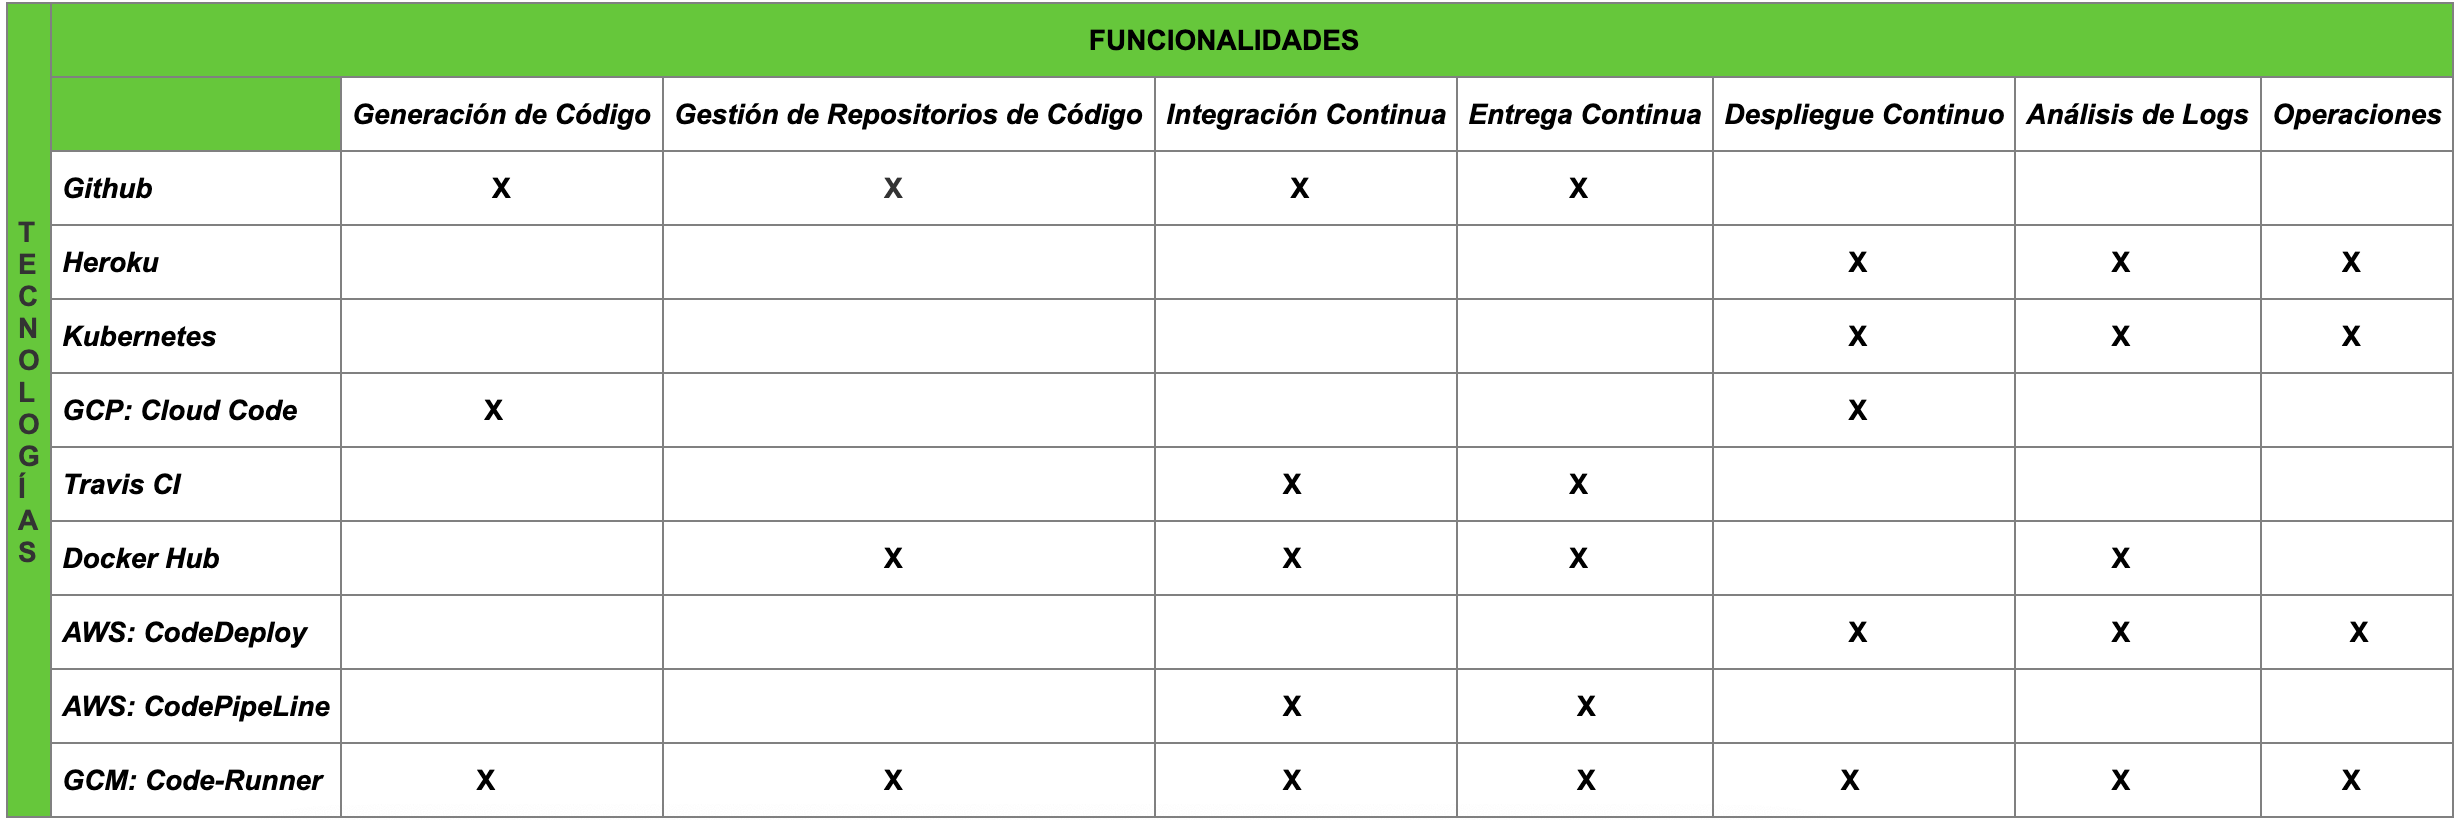
\includegraphics[scale=0.30]{imagenes/comparativa.png}
\caption{ Tabla Comparativa: Tecnología VS. Funcionalidad }
\end{figure}


\subsection{En este Proyecto}

Como se ha comentado en la introducción, las aplicaciones generadas por este sistema se caracterizan por ser aplicaciones del dominio de la web 2.0 es decir, aplicaciones accesibles a través de Internet por lo que la computación en la nube desarrolla un papel fundamental. 

En este proyecto se ha de diferenciar por una parte la infraestructura virtual y los recursos de la nube utilizados para poner a disposición de los usuarios  a través de Internet las aplicaciones generadas y por otra parte los recursos virtuales y de computación propios del sistema software necesarios para su correcto funcionamiento. 

Como se puede observar en las herramientas y tecnologías que están actualmente presentes en el mercado, es notable la necesidad de integrar y automatizar tareas relacionadas con el ciclo de vida del desarrollo software y las buenas prácticas. Aunque las herramientas presentadas tienen un gran alcance, ninguna presenta una solución completa como la que se presenta en este proyecto. Este sistema software pone a disposición de los usuarios un marco de trabajo generativo para crear y desplegar aplicaciones en unos sencillos pasos con el único requisito de poseer un perfil en Github. Para ello se integran diversas funcionalidades de servicios cloud como Github, Heroku y máquinas virtuales proporcionadas por la nube pública de Google  junto con Docker para construir un pipeline que permita generar y desplegar aplicaciones haciendo uso de las buenas prácticas anteriormente mencionadas. En la sección ~\ref{secid} Implementación y Desarrollo se justifica el uso de estas tecnologías. 

Está actividad de negocio entra dentro del tipo de servicio en la nube clasificado como Software as a Service\ref{secsaas} puesto que el usuario hace uso del sistema para consumir las aplicaciones que decide generar pero es abstraído del entorno virtual donde estas aplicaciones corren, es decir, el usuario trabaja a nivel de aplicación o servicio software. En la sección ~\ref{infra}  Infraestructura Virtual de las Aplicaciones se profundiza en estos conceptos y en la tecnología utilizada para su implementación. 

Por otra parte, para garantizar el correcto funcionamiento de este sistema software se requieren de los otros dos tipos de servicios en la nube. En la sección ~\ref{iv} Infraestructura Virtual se profundiza en los recursos de computación en la nube utilizados presentando los distintos entornos virtuales disponibles para que los usuarios puedan utilizar el sistema generativo.


\chapter{Planificación y Análisis}

\section{Planificación}

La planificación temporal muestra mediante el uso de diagramas de Gant la distribución en el tiempo de las tareas necesarias para cumplir con los objetivos de este proyecto. Los siguientes diagramas han sido confeccionados con la herramienta online Tom's Planner\cite{tom}

\begin{figure}[H]
\centering
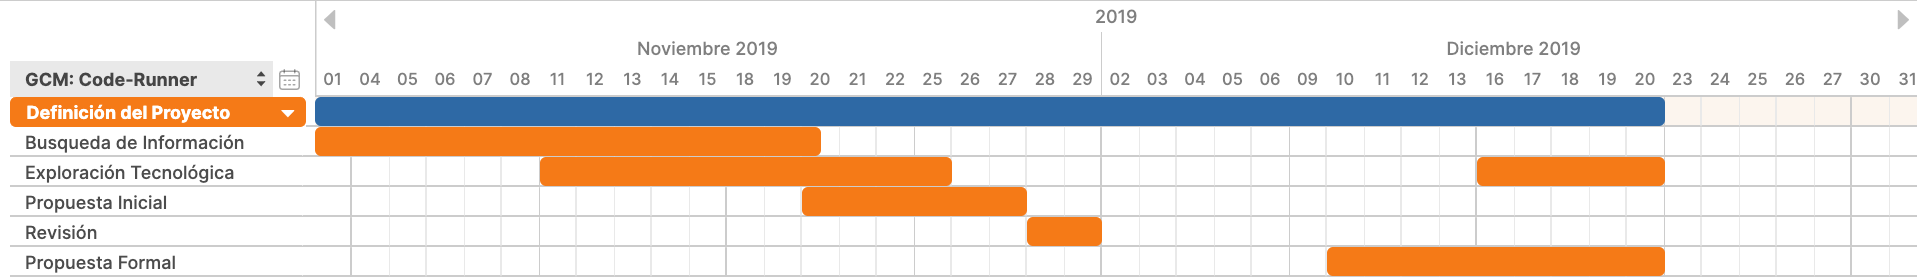
\includegraphics[scale=0.20]{imagenes/gant1.png}
\caption{ Planificación: Definición del Proyecto}
\end{figure}

\begin{figure}[H]
\centering
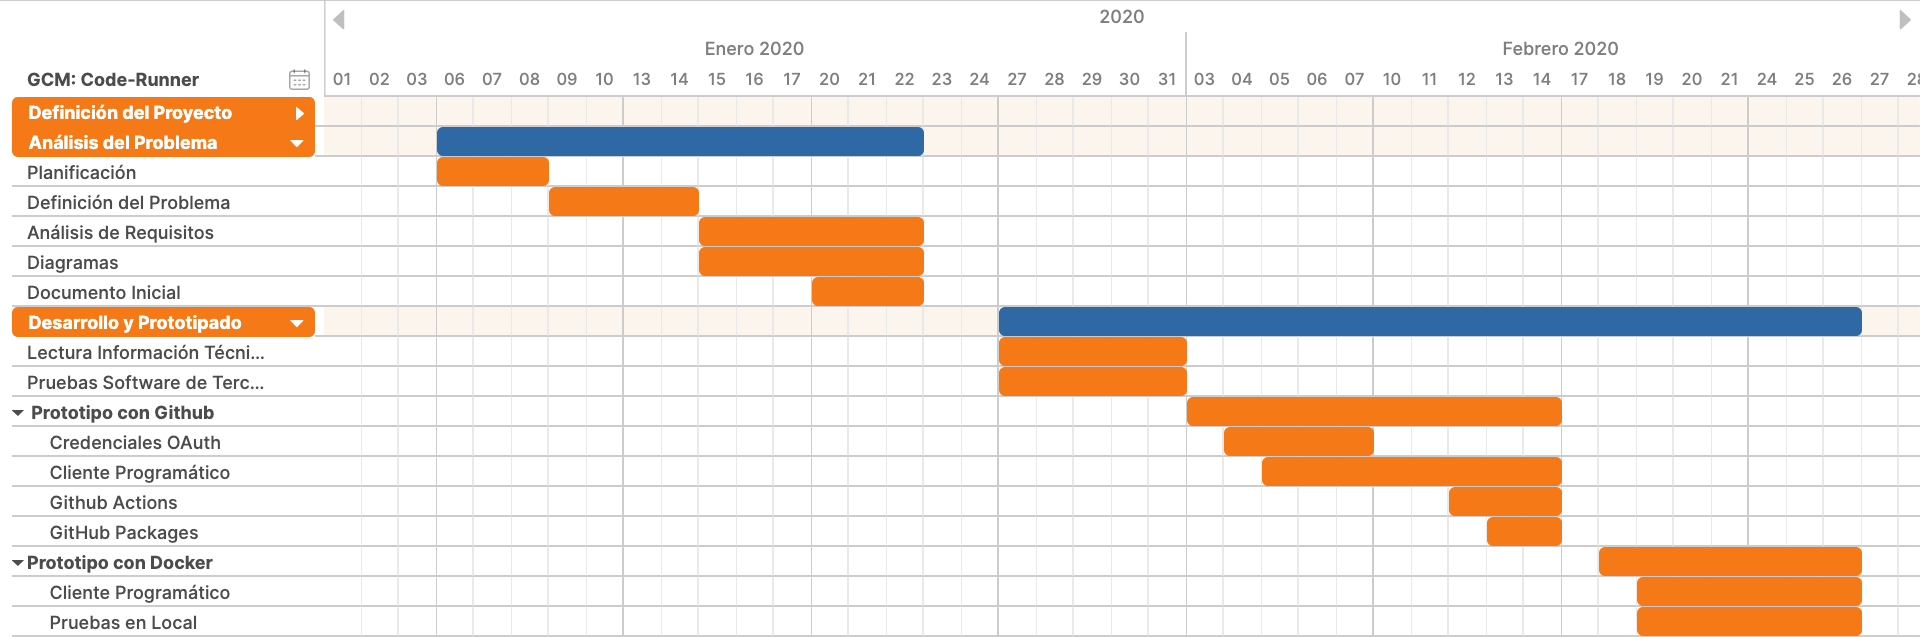
\includegraphics[scale=0.20]{imagenes/gant2.png}
\caption{ Planificación: Análisis y Desarrollo Inicial }
\end{figure}

\begin{figure}[H]
\centering
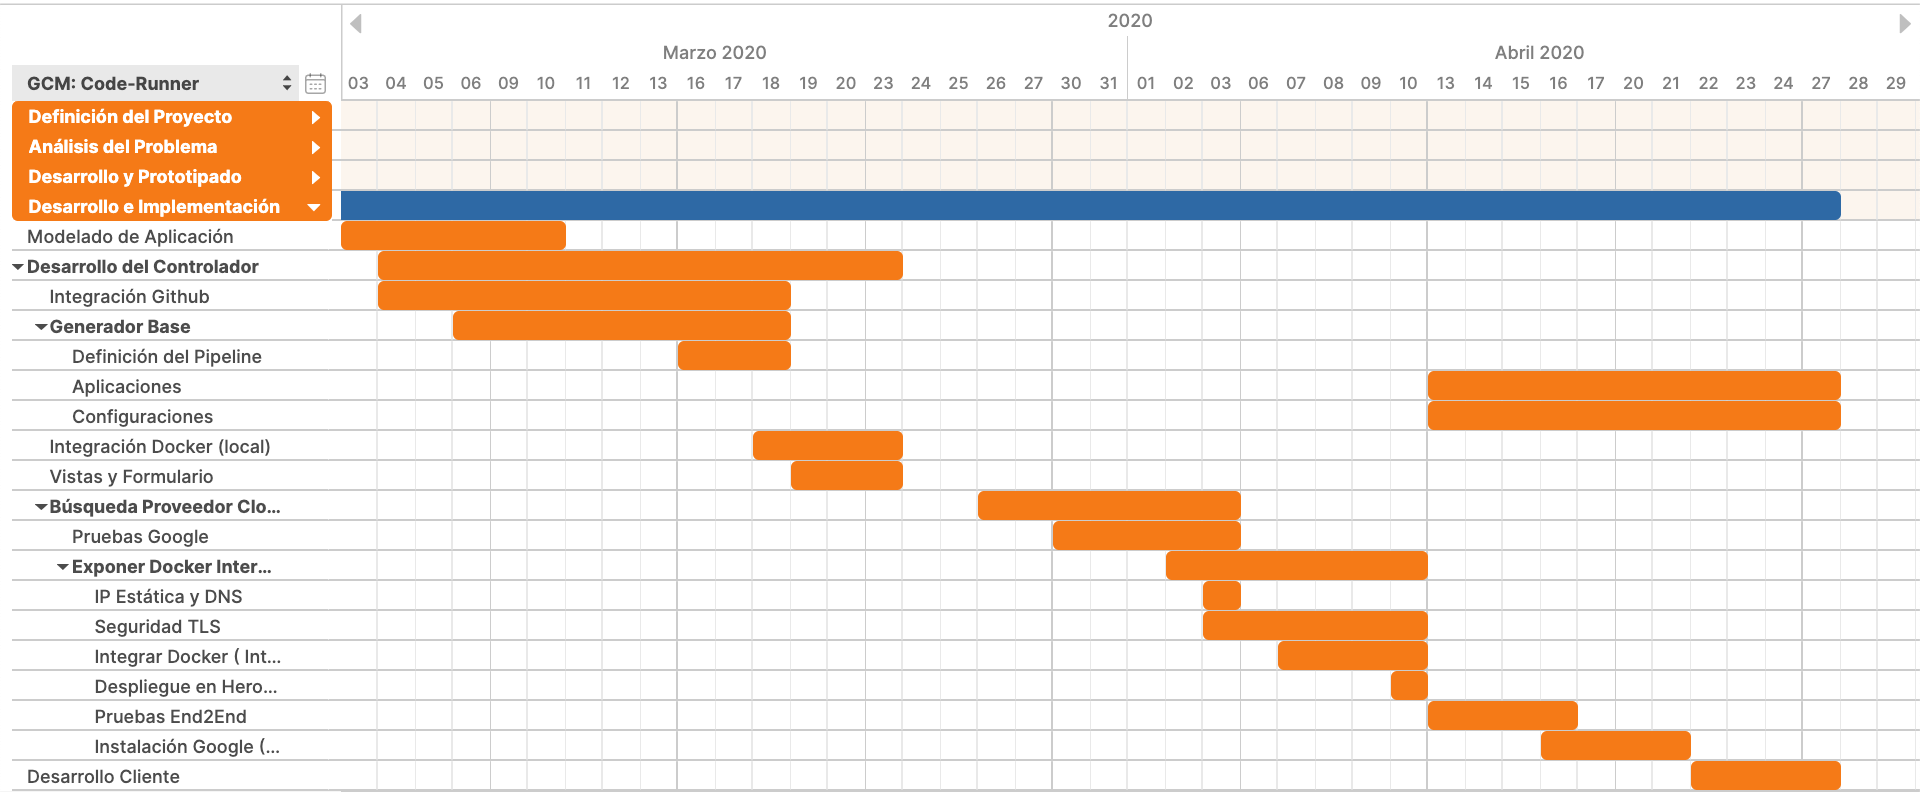
\includegraphics[scale=0.20]{imagenes/gant3.png}
\caption{ Planificación: Desarrollo Formal}
\end{figure}

\begin{figure}[H]
\centering
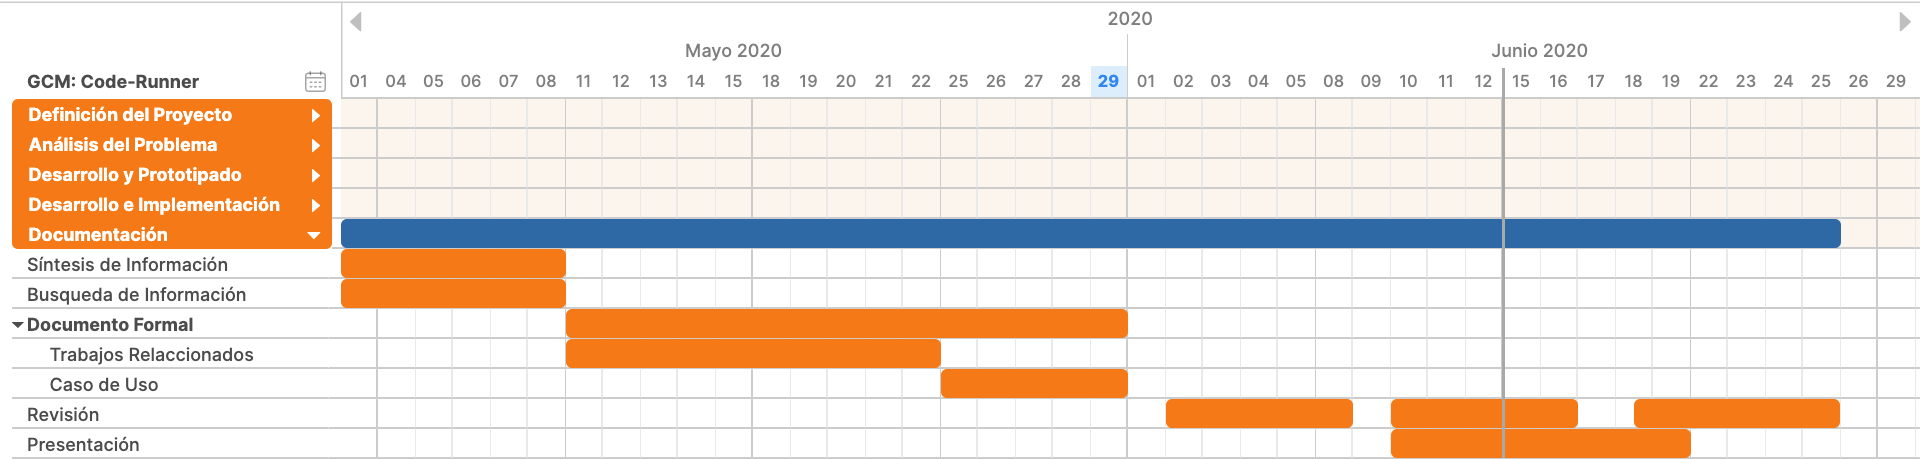
\includegraphics[scale=0.20]{imagenes/gant4.png}
\caption{ Planificación: Documentación Formal}
\end{figure}



\section{Análisis Software}

El análisis software pone de manifiesto la especificación del sistema software a construir. Dirigida por Ingeniería de requisitos y de casos de uso, las siguientes secciones muestran las partes y funcionalidades que el sistema resultante ha de cumplir.

\subsection{Requisitos de Información }
Los requisitos de información se caracterizan por reunir la información relevante para la solución, es decir, que debe gestionar y almacenar el sistema software.\\

\textbf{RI-1. Workspace:} Representación del espacio de trabajo del usuario. Contiene el conjunto de las aplicaciones que el usuario ha creado usando el sistema. Concepto similar al del Escritorio o "Desktop" de un sistema operativo.
Contenido: nombre de usuario o propietario del workspace, referencia al conjunto de aplicaciones generadas. \\
\textbf{RI-2. App:} Representación de cada una de las aplicaciones generadas por el sistema.
Contenido en Anexo: Modelo de Datos\ref{anexmodel}\\
\textbf{RI-3. Información de Usuario:} Información sensible del usuario o desarrollador que va a usar el sistema. Credenciales al sistema de gestión de repositorios para el código fuente, en este caso relativa al perfil de github.
Contenido: nombre de usuario, correo electrónico, organización. \\


\subsection{Requisitos Funcionales }
Como se define en la ingeniería de requisitos, los requisitos funcionales establecen el comportamientos del sistema.\\



\subsubsection { \textbf{ RF-1. Gestión de aplicaciones.}} El sistema ha de gestionar el ciclo de vida de las aplicaciones generadas.\\

\textbf{RF-1.1.} El sistema permitirá crear aplicaciones.
\begin{itemize}
 \item 	\textbf{RF-1.1.1.}El sistema generará aplicaciones de diversa naturaleza, tecnología o dominio. Añadir referencia a especificación de aplicaciones.
 \item 	\textbf{RF-1.1.2.}El sistema creará y  guardará en repositorios de código las aplicaciones generadas.
  \item \textbf{RF-1.1.3.}El sistema construirá los artefactos necesarios para ejecutar las aplicaciones generadas.
   \item  \textbf{RF-1.1.4.} El sistema ejecutará los artefactos construidos para disponibilizar vía Internet las aplicaciones creadas. \\
\end{itemize}


\textbf{RF-1.2.} El sistema permitirá eliminar aplicaciones.
\begin{itemize}
 \item 	\textbf{RF-1.2.1.}El sistema detendrá los artefactos en ejecución de aplicaciones eliminadas.
  \item 	\textbf{RF-1.2.2.}El sistema eliminará los artefactos construidos de aplicaciones eliminadas.
   \item  \textbf{RF-1.2.3.}El sistema eliminará los repositorios de código de aplicaciones eliminadas.	\\
\end{itemize}


\textbf{RF-1.3.} El sistema permitirá ejecutar aplicaciones.
\begin{itemize}
 \item \textbf{RF-1.3.1.} El sistema será capaz de hacer a las aplicaciones accesibles vía Internet.
 \item  \textbf{RF-1.3.2.} El sistema proporcionará las herramientas  y configuraciones necesarias para que las aplicaciones puedan ser ejecutas en local y ser accesibles vía \textbf{localhost}  \\
\end{itemize}


\textbf{RF-1.4.} El sistema permitirá detener aplicaciones.

\begin{itemize}
 \item  \textbf{RF-1.4.1.} El sistema será capaz de detener las aplicaciones que sean accesibles vía Internet.
  \item  \textbf{RF-1.4.2.} El sistema deberá liberar los recursos virtuales correspondientes a la aplicación detenida.
  \item  \textbf{RF-1.4.3.} El sistema proporcionará las herramientas  y configuraciones necesarias para que las aplicaciones ejecutadas en \textbf{localhost}  sean detenidas de manera controlada. \\
\end{itemize}

\textbf{RF-1.5.} El sistema permitirá visualizar información de las aplicaciones.

\begin{itemize}
\item \textbf{RF-1.5.1.} El sistema permitirá consultar  información de utilidad relativa a las aplicaciones,  como por ejemplo, especificación, URL del repositorio donde se alberga el código fuente, URL o IP donde la aplicación puede ser consumida vía Internet.
\item \textbf{RF-1.5.2.} El sistema permitirá inspeccionar aplicaciones. El sistema permitirá a los usuario consultar información de DEBUG de las aplicaciones accesibles vía Internet, es decir, permitirá consultar LOGs de aplicaciones en ejecución.
\item \textbf{RF-1.5.3.} El sistema permitirá visualizar información del estado del ciclo de vida de las aplicaciones. El ciclo de vida de las aplicaciones del sistema se representará con el siguiente flujo de estados:\\
\end{itemize}


\subsubsection { \textbf{ RF-2. Gestión de credenciales.}} El sistema proporcionará los mecanismos necesarios para que los usuarios se autentiquen en el sistema. \\


\textbf{RF-2.1.} El sistema  permitirá iniciar sesión  a los usuarios mediante nombre de usuario y contraseña. Típicamente estas credenciales corresponderán al sistema de gestión de repositorios de código.

\textbf{RF-2.3.} El sistema  permitirá cerrar sesión a los usuarios de manera controlada, es decir, mantendrá las aplicaciones en ejecución.

\textbf{RF-2.3.} El sistema  realizará todas las operaciones que requieran autenticación mediante TOKEN.

\textbf{RF-2.4.} El sistema  proporcionará a los usuarios el TOKEN necesario para trabajar localmente con las aplicaciones.


\subsection{Requisitos No Funcionales }
Los requisitos no funcionales, se refieren a todos los requisitos que no describen información a guardar, ni funciones a realizar por el sistema, sino características de funcionamiento.\\


\textbf{RNF-1} Se necesitará acceso a Internet para utilizar las funcionalidades del sistema.\\

\textbf{RNF-2} Se necesitará una cuenta en Github para utilizar las funcionalidades del sistema.\\

\textbf{RNF-3} Se prestará especial atención en la gestión de credenciales de los usuarios.\\

\textbf{RNF-4} Se prestará especial atención en la seguridad del  las aplicaciones expuestas a Internet.
\subsection{Casos de Uso}
Los diagramas de casos de uso, son diagramas UML que representan gráficamente a todos los elementos que forman parte del modelo de casos de uso junto con la frontera del sistema. Delimitan el sistema a diseñar. Determinan el contexto del uso del sistema. Describen el punto de vista de los usuarios  en el sistema.


\begin{figure}[H]
\centering
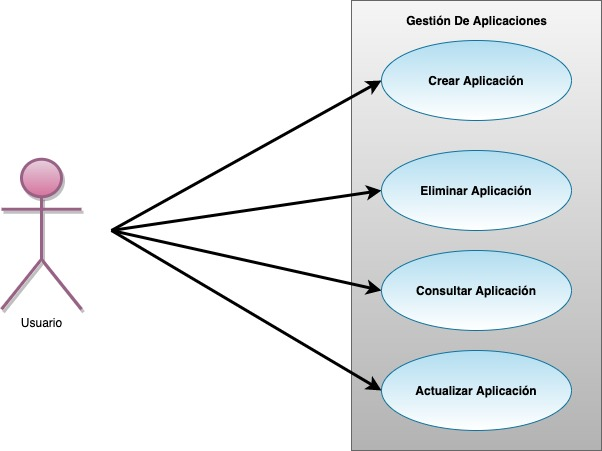
\includegraphics[scale=0.50]{imagenes/casosUso1.jpg}
\caption{ Casos de uso - Gestión Aplicaciones I\cite{diagrama}  }
\end{figure}

\begin{figure}[H]
\centering
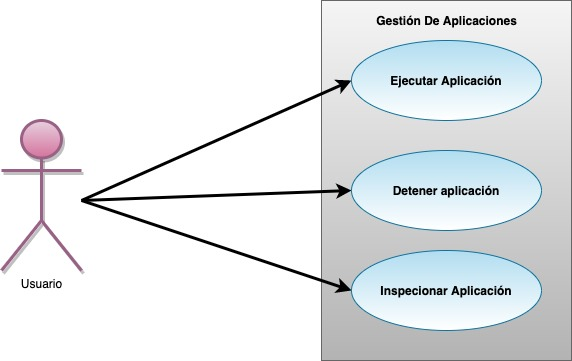
\includegraphics[scale=0.50]{imagenes/casosUso2.jpg}
\caption{ Casos de uso - Gestión Aplicaciones II\cite{diagrama}  }
\end{figure}

\begin{figure}[H]
\centering
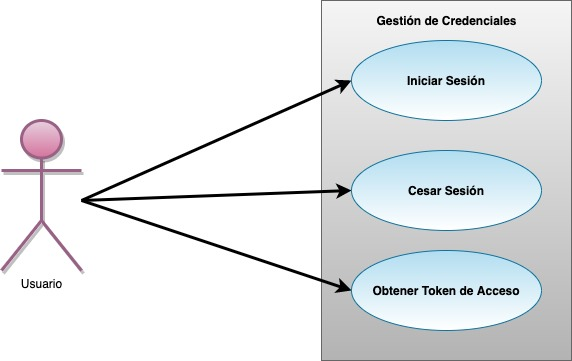
\includegraphics[scale=0.50]{imagenes/casosUso3.jpg}
\caption{ Casos de uso - Gestión Credenciales\cite{diagrama}  }
\end{figure}

\subsection{Diagramas de Secuencia}
Los diagramas de secuencia especifican las interacciones temporales entre las piezas internas del sistema para cumplir con las funcionalidades requeridas. Normalmente la tecnología que implementa cada una de las piezas internas del sistema no es incluida en este tipo de diagramas pero en este caso se incluye para mejorar la compresión del sistema por parte del lector. 


\begin{figure}[H]
\centering
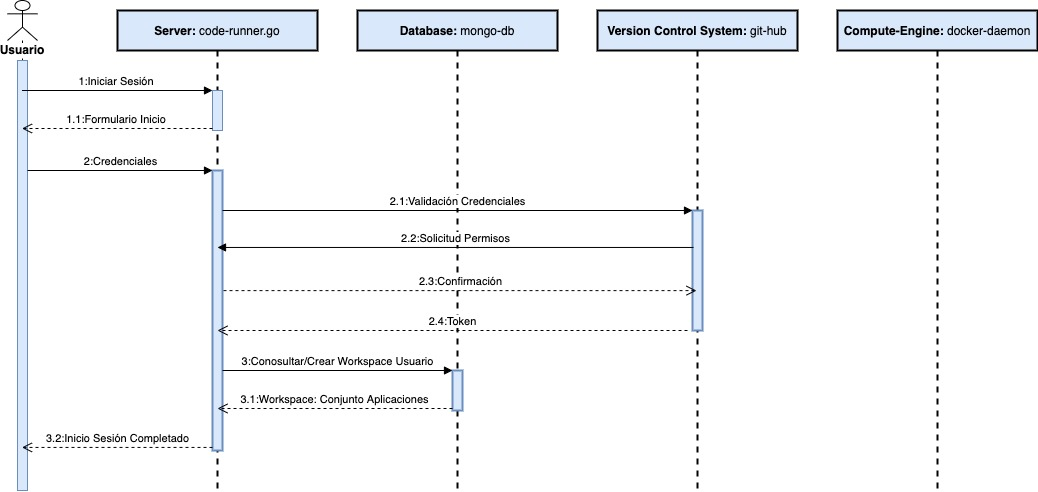
\includegraphics[scale=0.45]{imagenes/secuencia1.jpg}
\caption{ Diagramas de Secuencia - Inicio sesión \cite{diagrama}  }
\end{figure}

\begin{figure}[H]
\centering
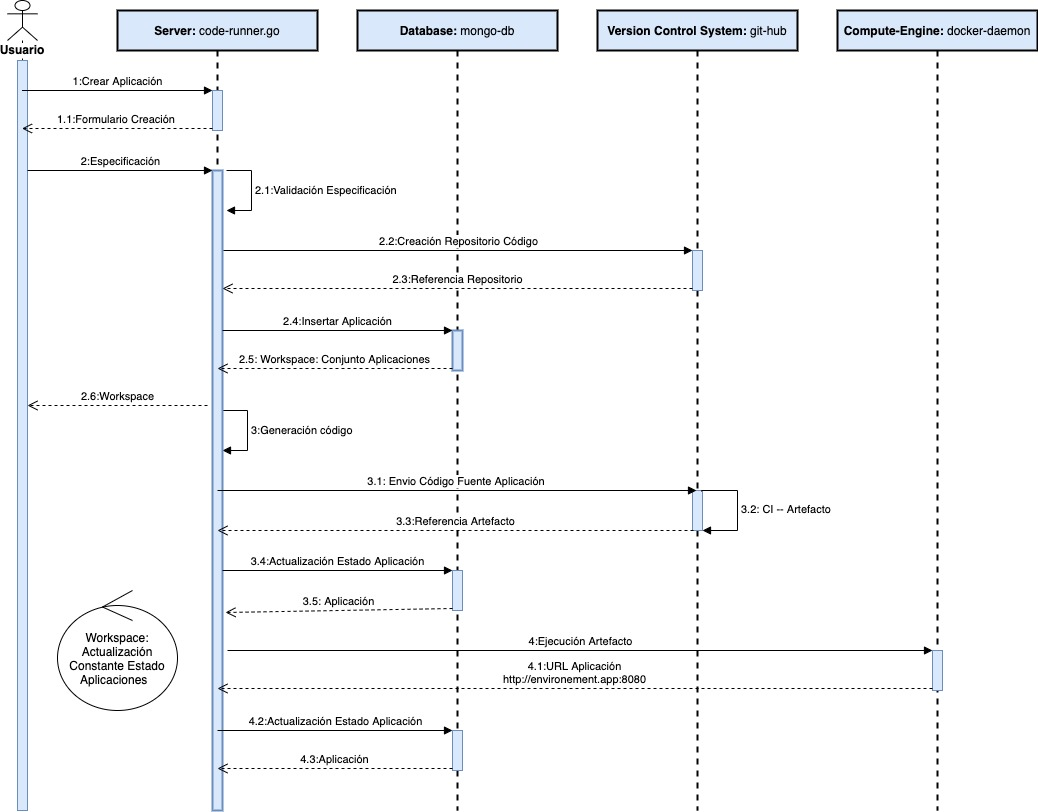
\includegraphics[scale=0.43]{imagenes/secuencia2.jpg}
\caption{ Diagramas de Secuencia - Crear Aplicación\cite{diagrama}  }
\end{figure}


\begin{figure}[H]
\centering
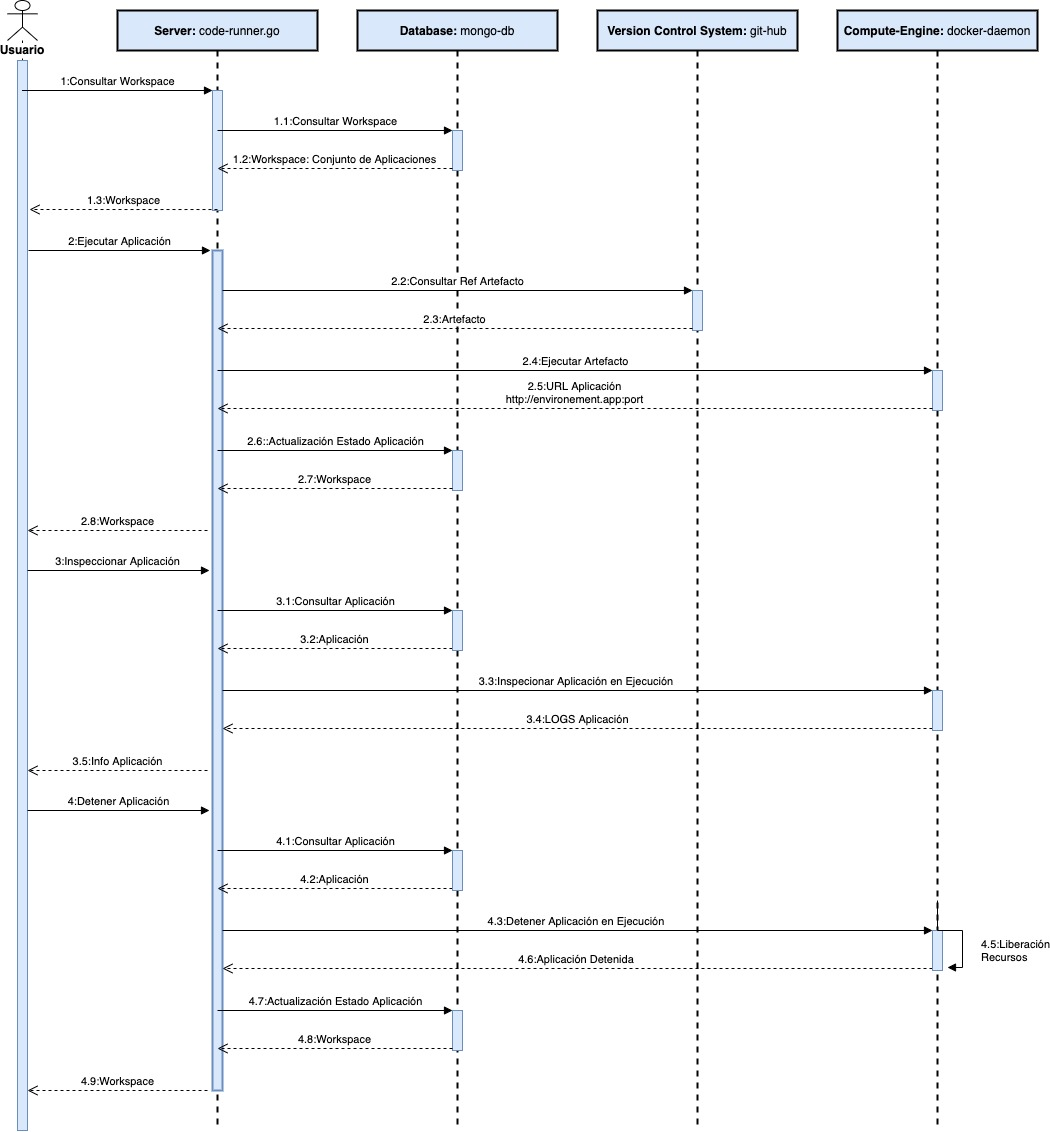
\includegraphics[scale=0.43]{imagenes/secuencia3.jpg}
\caption{ Diagramas de Secuencia - Ejecutar, Inspeccionar y Detener Aplicación\cite{diagrama}  }
\end{figure}

\begin{figure}[H]
\centering
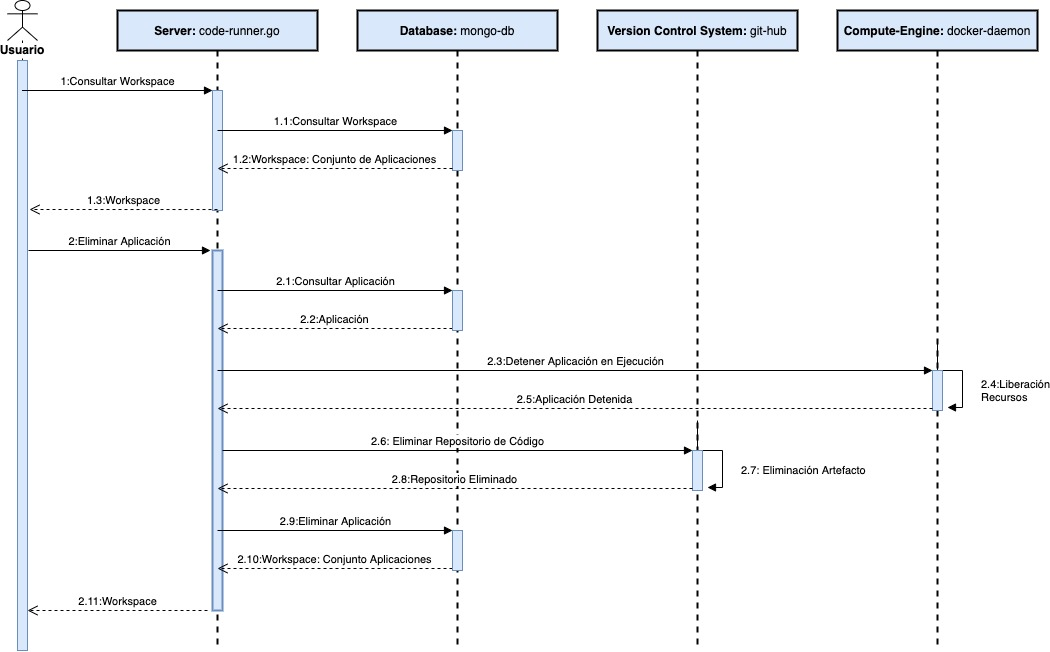
\includegraphics[scale=0.43]{imagenes/secuencia4.jpg}
\caption{ Diagramas de Secuencia - Eliminar Aplicación\cite{diagrama}  }
\end{figure}





\chapter{ Implementación y Pruebas}


\section{Implementación y Desarrollo}\label{secid}

En el proceso de desarrollo e implementación del sistema, se ha seguido el patrón de arquitectura software modelo-vista-controlador (MVC)\cite{mvc} cuya finalidad es separar los datos y la lógica de una aplicación de la interfaz de usuario. Este patrón de arquitectura se basa en la re-utilización de código y separación de conceptos. El objetivo de esta metodología es el de facilitar el desarrollo, mantenimiento y escalabilidad del software resultante.

\begin{figure}[H]
\centering
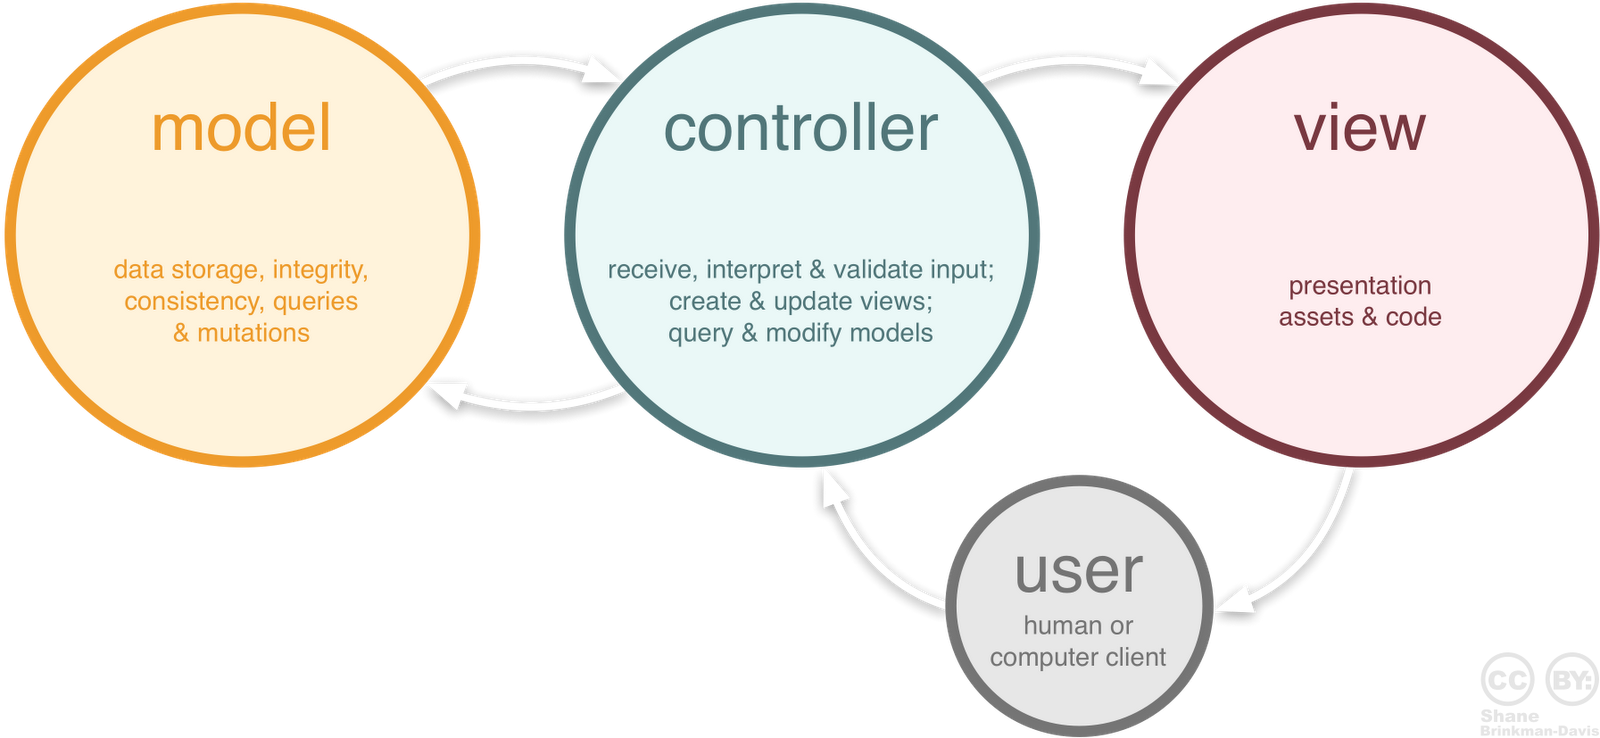
\includegraphics[scale=0.20]{imagenes/mvc.png}
\caption{ Modelo-Vista-Controlador\cite{mvc2}  }
\end{figure}

Los componentes\cite{mvc3} del Modelo-Vista-Controlador se pueden definir en:

\begin{enumerate}
\item \textbf{Modelo:} Representa la información, gestionando los accesos a ella, la base de datos  o capa de persistencia es un componente del modelo.

\item \textbf{Vista:} Representa el modelo en un formato adecuado para interactuar con él mediante la interfaz de usuario.

\item \textbf{Controlador:} Responde a eventos invocando peticiones al modelo cuando se hace alguna solicitud de la información (por ejemplo, editar un documento o un registro en base de datos). El controlador interactúa con su vista asociada para realizar cambios en la forma de representar el modelo.
\end{enumerate}

Como parte del desarrollo del proyecto también se ha utilizado la metodología de ingeniería del software conocida como desarrollo basado en test o TDD. Dicha metodología consiste en escribir los test necesarios para cubrir las funcionalidades del sistema y a partir de ellos, escribir el código necesario para que dichas pruebas sean superadas, cumpliendo así la funcionalidad que se esta poniendo a prueba.  En las siguientes secciones se detallan las partes que forman el sistema así como las tecnologías utilizadas. 

\subsection{Back-End}

El Back-End o servidor se refiere a la parte trasera del sistema, donde ocurre toda la lógica y funcionalidad pero que es transparente para el usuario final que consume el sistema. Para facilitar la comprensión de las partes que forman  el Back-End del proyecto se van a desglosar en las siguientes secciones.

\subsubsection{Servidor}

El servidor es la entidad principal del Back-End, contiene la lógica del sistema y es el responsable de la comunicación entre el resto de componentes del sistema y de servir o renderizar las vistas al cliente.
El servidor ha sido desarrollado utilizando Golang\cite{go} como lenguaje de programación. Inicialmente se pensó en utilizar JavaScript bajo el framework Node.JS, ya que dicho marco de trabajo funciona de manera asíncrona, lo que facilita muchas de las operaciones en segundo plano que este sistema ha de realizar, ademas Node.JS facilita la integración del servidor con diversas tecnologías cliente basadas también en JavaScript. Una de las principales deficiencias  observadas en el uso de JavaScript para el desarrollo del servidor de este proyecto es el manejo de plantillas para el generador de código por lo que este lenguaje fue descartado.

En la etapa de generación de código la templatización de los modelos de datos necesarios para producir aplicaciones es vital, no solo en su implementación si no también en la eficiencia de estas operaciones y es aquí donde Golang destaca, ya que permite serializar estructuras de datos complejas y utilizar dicha representación para crear contenido. Otra ventaja que proporciona utilizar Golang en este proyecto es el uso de Go-Routinas, es decir, la capacidad de ejecutar funcionalidad en segundo plano de una manera sencilla y controlada junto con la generalización que se alcanza al usar interfaces. Estos motivos hacen que Golang sea el lenguaje de programación adecuado para el desarrollo de este proyecto.  Es interesante destacar que Golang ha sido diseñado para optimizar el uso concurrente de las aplicaciones creadas con él, lo que mejora considerablemente los tiempos de respuesta y la experiencia de usuario de cara a que el proyecto sea utilizado por numerosos clientes a través de Internet.

\subsubsection{Persistencia de Datos}

La parte imprescindible para la capa de acceso a datos es el sistema gestor de bases de datos, encargado de almacenar los modelos del sistema. Como propuesta inicial para el desarrollo del sistema, se pensó en utilizar un esquema relacional utilizando sistemas gestores de bases de datos relacionales como MySQL o PostgreSQL  por la facilidad de diseño e implementación basada en entidad-relación.

La principal desventaja de modelar el problema mediante entidad-relación es la perdida en la flexibilidad de los modelos de datos ya que este esquema tradicional obliga a que todas las filas de una tabla representativa de un modelo tengan los mismos campos para mantener la entidad referencial y debido a la diversidad de aplicaciones que este sistema es capaz de generar se requiere que el modelo de datos sea flexible. Debido a esto, se ha decido utilizar MongoDB\cite{mg} como sistema gestor de bases de datos no-relaciones también denominadas bases de datos documentales, con el objetivo de conseguir un esquema interno flexible y eficiente. Es decir, el modelo de aplicación que el usuario define para generar aplicaciones podría ser evolucionado y mejorado sin romper el esquema actual. 

\begin{figure}[H]
\centering
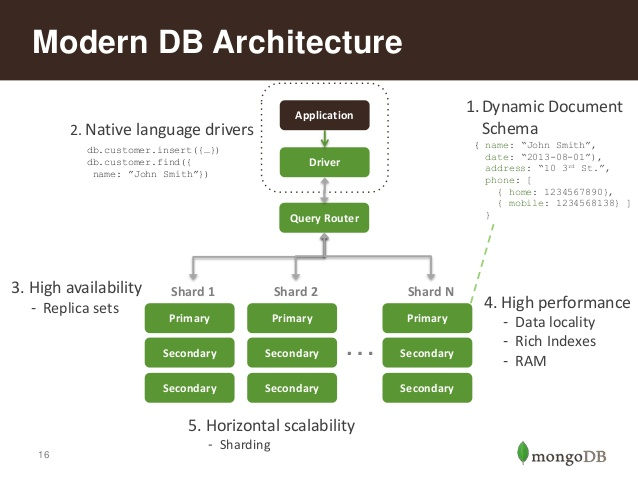
\includegraphics[scale=0.30]{imagenes/mongo.jpg}
\caption{ Arquitectura MongoDB\cite{mongoA}  }
\end{figure}

MongoDB es un sistema de base de datos NoSQL orientado a grandes cantidades de datos, guarda estructuras de datos en documentos similares a JSON. Se trata de una base de datos ágil que permite cambiar los esquemas de una aplicación cuando esta evoluciona. Los principales objetivos de estas bases de datos son la escalabilidad, rendimiento y gran disponibilidad.

En MongoDB los documentos se agrupan en colecciones. Las colecciones  no imponen una estructura fija a los documentos que contienen, ni siquiera al tipo de datos de cada campo. Esto es una ventaja cuando las entradas de la base de datos dependen de la naturaleza de las aplicaciones que el usuario final quiera generar.


\subsubsection{Repositorio de Código}\label{repo}

Las entidades generadas por este sistema ( aplicaciones) están compuestas por un conjunto de ficheros ( README, licencia, código fuente, configuración, scripts, makefile, dockerfile...etc), estos ficheros producidos por el sistema son almacenados en repositorios de código alojados en la nube de manera pública, para ello, este proyecto esta completamente integrado con Github\cite{github} aprovechando de este gestor de repositorios las siguientes funcionalidades: 

\begin{enumerate}
\item \textbf{ Autenticación.} El usuario final que utilice este sistema para generar aplicaciones necesita una cuenta de Github, ya que la autenticación mediante usuario y contraseña corresponde con el las credenciales  de su perfil de Github. Esto permite al sistema crear repositorios y subir el código generado a dichos repositorios bajo el perfil del usuario registrado. El proceso de autenticación contra Github proporciona una Token  de acceso el cual es aprovechado por una parte por el sistema generativo para realizar llamadas a la API  de Github y automatizar ciertas operaciones en nombre del usuario final y por otra parte los usuarios finales del sistema  pueden utilizar este Token para trabajar localmente con las aplicaciones generadas por el sistema.

\item   \textbf{Integración Continua.} Github proporciona las denominadas GitHub-Actions\cite{github3}  que permiten automatizar, personalizar y ejecutar flujos de integración continua  sobre los proyectos software alojados en sus repositorios, para ello, en el proceso de Code Generatión este sistema produce un fichero  en la ruta:\\
\textbf{repositorio/.github/workflows/ci.yml}\ref{anexci} donde se describe el proceso o etapas de compilación, testing y empaquetado del la aplicación contenida en el repositorio, independientemente de la naturaleza de la aplicación, dando lugar a un artefacto auto-contenido listo para ser desplegado sobre un entorno virtual. Esto garantiza el uso de las buenas prácticas  de integración y entrega continua relativas al desarrollo software en todas las aplicaciones generadas.

\item \textbf{Gestión de Artefactos} Github proporciona los denominados GitHub-Packages\cite{github4} que permiten publicar y consumir paquetes o artefactos resultado de la compilación y empaquetado de las aplicaciones software albergadas en un repositorio de código. GitHub-Packages es capaz de gestionar paquetes de diversa naturaleza, siendo las imágenes docker las utilizadas en este proyecto.
\end{enumerate}

\subsubsection{Infraestructura Virtual de las Aplicaciones}\label{infra}

La infraestructura virtual de las aplicaciones  representa al entorno de computación en la nube que cuenta con los recursos necesarios para ejecutar o desplegar las aplicaciones generadas por el proyecto, permitiendo a los usuarios utilizar las aplicaciones generadas vía Internet.
Con el objetivo de generalizar la gestión de aplicaciones  se ha decidido utilizar Docker como tecnología de virtualización ligera.

Docker\cite{dk} es una herramienta para automatizar el despliegue de aplicaciones dentro de contenedores, proporcionando una capa de abstracción y automatización de virtualización a nivel de sistema operativo. Docker utiliza aislamiento de recursos del kernel de sistemas Unix  para permitir que contenedores independientes se ejecuten dentro de una sola máquina, evitando la sobrecarga de iniciar y mantener máquinas virtuales completas.

\begin{figure}[H]
\centering

\includegraphics[scale=0.35]{imagenes/docker.png}
\caption{ Virtualización Docker\cite{dkw}}
\end{figure}

La principal diferencia con respecto a máquinas virtuales es el tamaño. Las máquinas virtuales incluyen la aplicación, el código, las librerías necesarias y un sistema operativo anfitrión completo mientras que los contenedores disponen de recursos similares pero de manera compartida con el núcleo  del sistema operativo anfitrion y junto con otros contenedores los cuales se ejecutan  como procesos asilados en el espacio de usuario del sistema operativo. No están vinculados con ninguna infraestructura especifica.

Docker aporta a este proyecto la capacidad de abstraer las aplicaciones de la infraestructura virtual subyacente. En la etapa de Code Generation se produce un fichero denominado Dockerfile con la definición necesaria para ejecutar la aplicación producida en un contenedor. Este fichero es aprovechado  por el flujo de integración y entrega continua de la aplicación  para producir una imagen docker como artefacto. Este artefacto es utilizado para crear un contenedor docker en un entorno virtual accesible a Internet( máquina virtual), habilitando el puerto necesario para garantizar que el trafico es re-direccionamiento al contenedor correspondiente y de esta manera permitir que el usuario del sistema generativo consuma a través de Internet la aplicación generada, siendo todo esto trasparente para él. 


\subsection{Front-end}

El Front-End, capa de presentación o capa de cliente es la encargada de controlar la interacción con el usuario. En este proyecto la programación en el lado cliente se utiliza para mantener  información actualizada del estado en el que se encuentran las aplicaciones producidas por el sistema. Para ello, se aprovecha el motor de plantillas proporcionado por el servidor Golang junto con JQuery y Ajax para realizar llamadas asíncronas al servidor y actualizar dinámicamente los datos que percibe el cliente. De manera adicional, el sistema proporciona una consola de monitorización  que permite al usuario inspeccionar en tiempo real los logs de su aplicación así como el tráfico que dicha aplicación está soportando usando para ellos WebSockets. 

\subsubsection{Tecnología Cliente}


JQuery\cite{jq} es una librería de JavaScript, que permite interactuar con los documentos HTML, manipular el árbol DOM, manejar eventos, desarrollar animaciones y agregar interacción con el servidor mediante llamadas asíncronas realizadas con Ajax. Su objetivo principal es dar un comportamiento dinámico a la web. Jquery funciona en múltiples navegadores y es compatible con CSS3.

Ajax\cite{aj}, abreviatura de JavaScript Asíncrono y XML es un conjunto de técnicas de desarrollo web en el cliente para crear aplicaciones asíncronas y dinámicas. Con Ajax, las aplicaciones pueden enviar y recibir datos desde el servidor en segundo plano sin que interfiera en la visualización o el comportamiento de la aplicación. Utilizar Ajax supone crear aplicaciones web en las que la capa de intercambio de datos ha sido separada de la capa de presentación, lo que permite un comportamiento dinámico sin la necesidad de recargar el navegador.


WebSocket es un tecnología basada en JavaScript que permite la comunicación bidireccional entre cliente y servidor mediante un único enlace TCP. Los WebSockets pueden entenderse como una evolución de Ajax, ya que permiten recopilar información del servidor sin tener que solicitarla expresamente, es decir, la información del servidor fluye hasta el cliente cuando esta es producida por lo que es ideal para implementar la consola de inspección en tiempo real. Para ello, desde la capa cliente se abre un socket TCP con el servidor, el cual emite por este canal toda la información que el docker de la aplicación produce al atender peticiones.  

Por último destacar que para los estilos de la capa cliente se ha utilizado la librería CSS Bootstrap\cite{boot}

\subsection{Infraestructura Virtual}\label{iv}

Para que el sistema software sea consumido por los clientes se han disponibilizado dos entornos independientes con las siguientes características:

\subsubsection{Entorno de Desarrollo}

El entorno\url{https://coderunner.herokuapp.com/} ha estado disponible desde el comienzo de la etapa formal del proyecto. El objetivo de este entorno es el de facilitar el proceso de desarrollo ya que  como se ha visto en los diagramas de caso de uso y en la sección anterior dedicada al Back-End, el sistema esta compuesto por 4 piezas principales y ha sido necesario disponer de ellas en Internet para trabajar en su integración y comportamiento de cara a cumplir con los requisitos propuestos. Este entorno se caracteriza por la siguiente distribución: 


\begin{enumerate}
\item Servidor principal (code-runner.go): Desplegado en Heroku\cite{hero}
\item Capa de persistencia (MongoDB): Consumido desde el servicio de bases de datos gestionadas \url{https://mlab.com}
\item Gestor de repositorios: Github\cite{github}
\item Demonio Docker: Maquina virtual expuesta a Internet con TLS sobre el proveedor de nube publica Google Cloud(trial)\cite{gcp}
\end{enumerate}

El objetivo de esta configuración ha sido el de conseguir el conjunto de recursos virtuales necesarios para el proyecto con el menor gasto posible (0€)

\subsubsection{Entorno Formal}

El entorno\url{https://apps.gcm-coderunner.com/} ha sido creado en las últimas etapas del proyecto, teniendo claras las necesidades a cubrir y prestando especial atención a los posibles cuellos de botella, como puede ser la capacidad de las máquinas virtuales expuestas a Internet para instanciar contenedores.  También se ha prestado especial atención en implementar medidas de seguridad como es el uso de certificados (TLS) o el no consumir servicios de terceros para la capa de persistencia y servir MongoDB de manera asilada. Este entorno se caracteriza por la siguiente distribución: 

\begin{enumerate}
\item Servidor principal (code-runner.go): Desplegado en VM de GoogleCloud\cite{gcp}
\item Capa de persistencia (MongoDB): Instalada en la misma VM donde corre el servidor principal y expuesta solo para ser consumida por procesos ejecutados en localhost. 
\item Gestor de repositorios: Github\cite{github}
\item Demonio Docker: Ejecutado en la misma VM que el servidor principal  pero expuesto con TLS a localhost, limitando de esta forma los posibles ataques externos que reciba el sistema, pues solo se exponen a Internet los contenedores de los usuarios, no el servicio de contenedores en si. 
\end{enumerate}


El objetivo de esta configuración ha sido el de conseguir el conjunto de recursos virtuales necesarios para el proyecto prestando especial atención a la seguridad y también a la capacidad, ya que el dimensionamiento de las VMs de este entorno es notablemente superior al de el entorno de desarrollo lo que permite la ejecución de números contenedores por diversos usuarios concurrentes.  El mantenimiento de este entorno produce gasto directamente proporcional al dimensionamiento de las máquinas virtuales que se utilizan así como el nombre de dominio usado. 

\subsection{Seguridad}

\subsubsection{Credenciales de Usuario}

Como se indicó anteriormente, las credenciales de usuario necesarias para utilizar el sistema se corresponden con las credenciales del perfil del usuario en Github. Esto es así debido a que la autenticación (¿Quien es usted?) y la autorización (¿Qué le permite usted hacer al sistema sobre sus repositorios de código?) son delegadas a Github mediante las denominado OAuth Apps. Una aplicación OAuth consise en autenticación delegada a terceros, es decir, cuando el usuario comienza a utilizar este sistema, los servidores de Github validan sus credenciales y emiten un token de acceso con el que realizar operaciones vía API. Este token es almacenado en una sesión del servidor con un tiempo de espiración determinado. 

\subsubsection{Comunicación Cliente-Servidor}

Este proyecto implementa Transport Layer Security (TLS) para garantizar que la información intercambiada entre el servidor y los clientes es segura y viaja encriptada exponiendo su servicio mediante protocolo HTTPS. Por otra parte, la comunicación del servidor con el demonio docker donde se ejecutan las aplicaciones generadas por el usuario también utiliza TLS.

\section{Caso de Uso}

Para mostrar las capacidades del sistema software \textbf{GCM:Code-Runner} se presenta el siguiente caso de uso desglosado en las distintas operaciones que el usuario final es capaz de realizar sobre el sistema en cualquiera de los dos entornos disponibles:

\begin{enumerate}
\item \url{https://apps.gcm-coderunner.com}
\item \url{https://coderunner.herokuapp.com}
\end{enumerate}

En este caso de uso se va a utilizar el primero de ellos por ser mas seguro y disponer de un dimensionamiento mayor (mejores prestaciones).

\subsection{Autenticación y Autorización}

Como paso inicial, el usuario ha de autenticarse y autorizar al sistema a realizar operaciones sobre sus repositorios de código. Para ello, desde un explorador web ha de navegar hasta \url{https://apps.gcm-coderunner.com}. Se presenta la pagina de bienvenida. 

\begin{figure}[H]
\centering
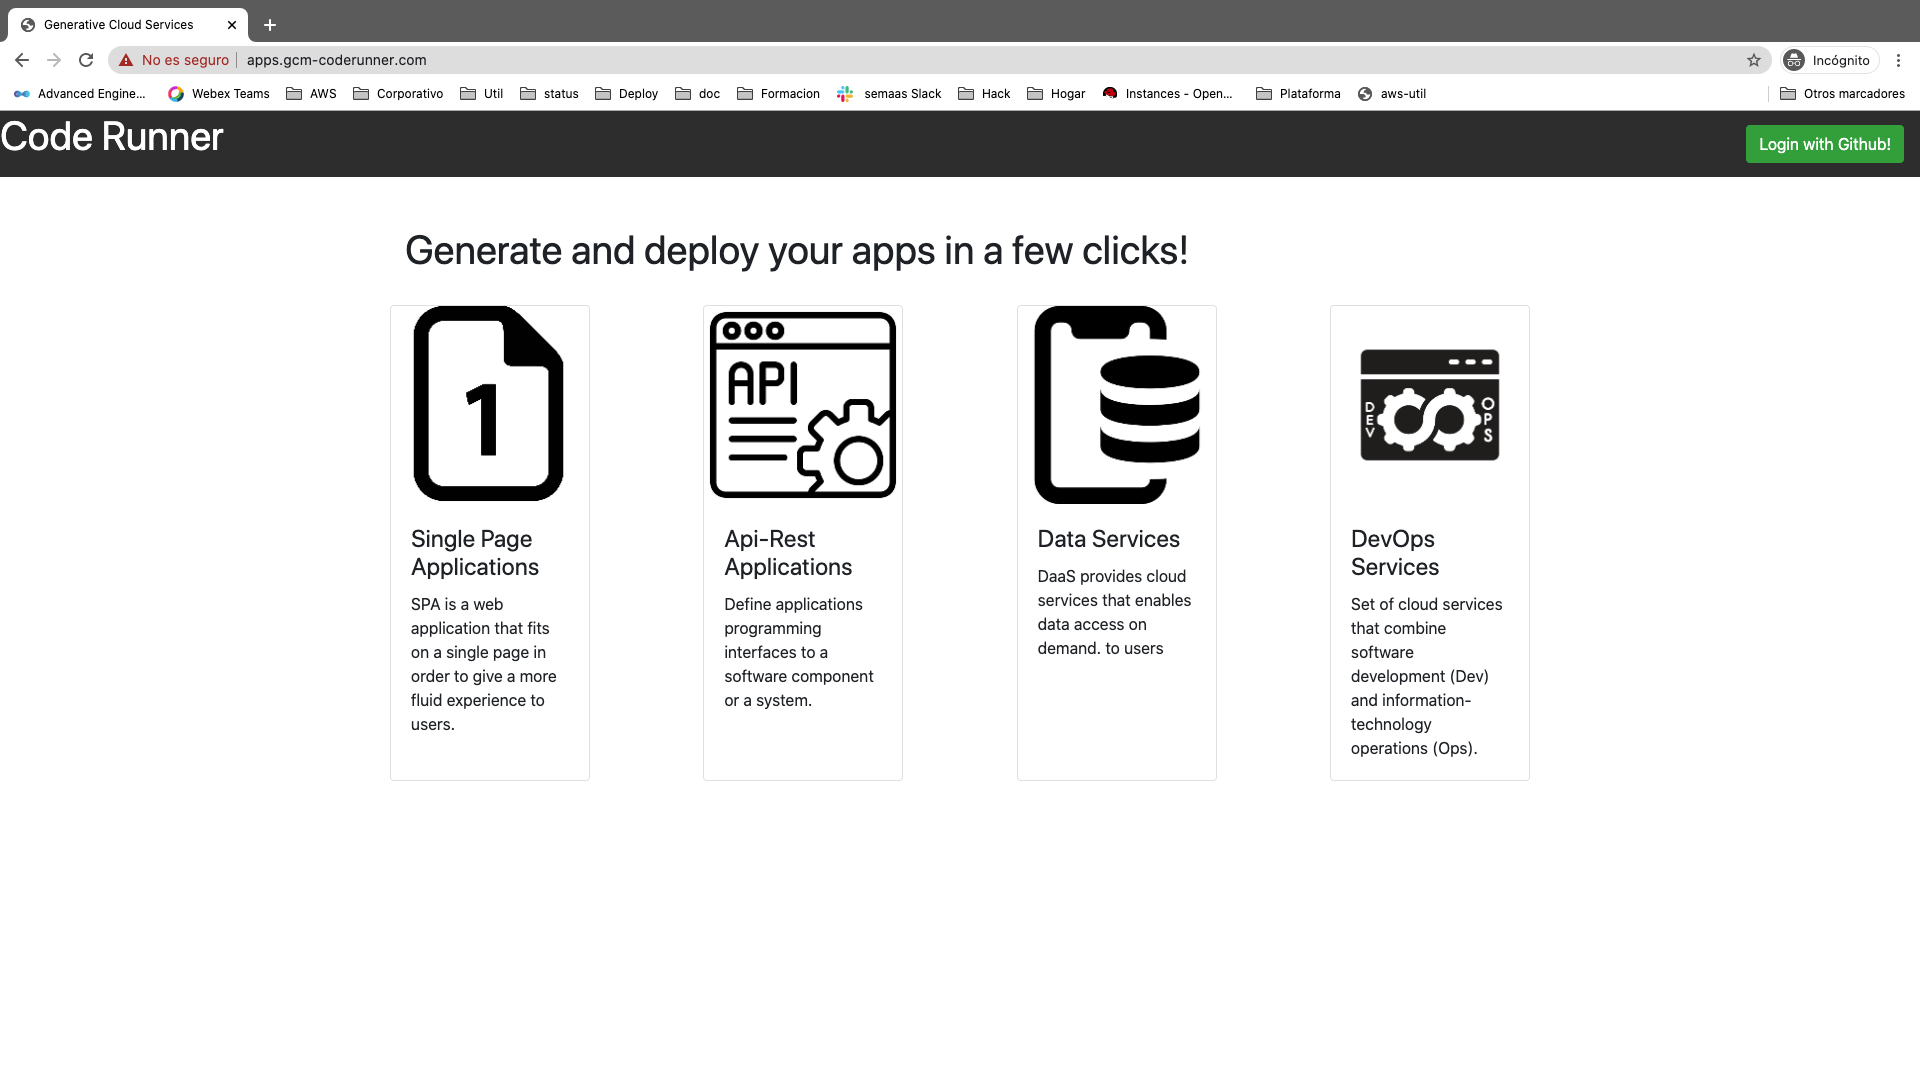
\includegraphics[scale=0.2]{imagenes/casouso/1.png}
\caption{  Autenticación y Autorización: Index }
\end{figure}

Para iniciar sesión, es necesario hacer click en el botón de \textbf{Login with Github} y el proceso de autenticación es delegado a este servicio:

\begin{figure}[H]
\centering
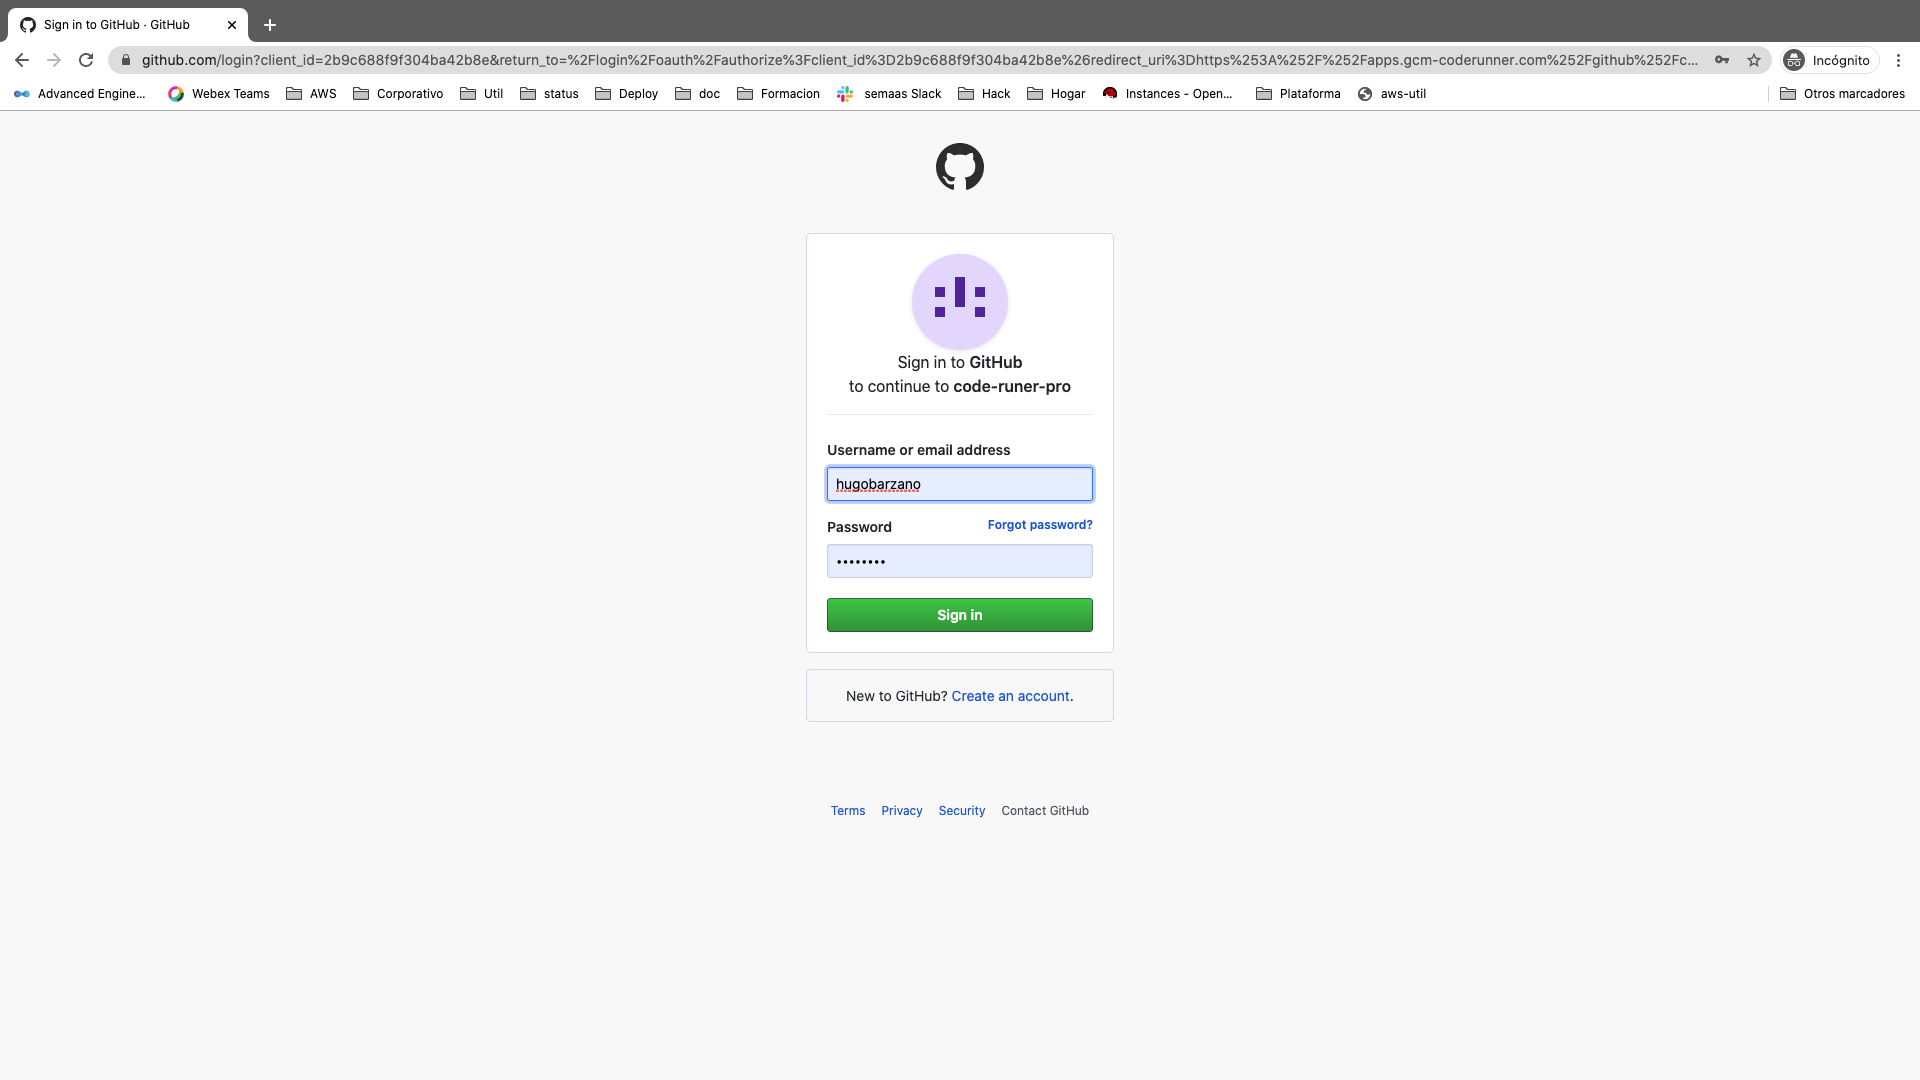
\includegraphics[scale=0.2]{imagenes/casouso/2.png}
\caption{  Autenticación y Autorización: Autenticación }
\end{figure}

Es necesario introducir usuario y contraseña correspondientes al perfil de Github. Haciendo click en el botón de  \textbf{Sign In} el mecanismo de autenticación continua con la autorización: 

\begin{figure}[H]
\centering
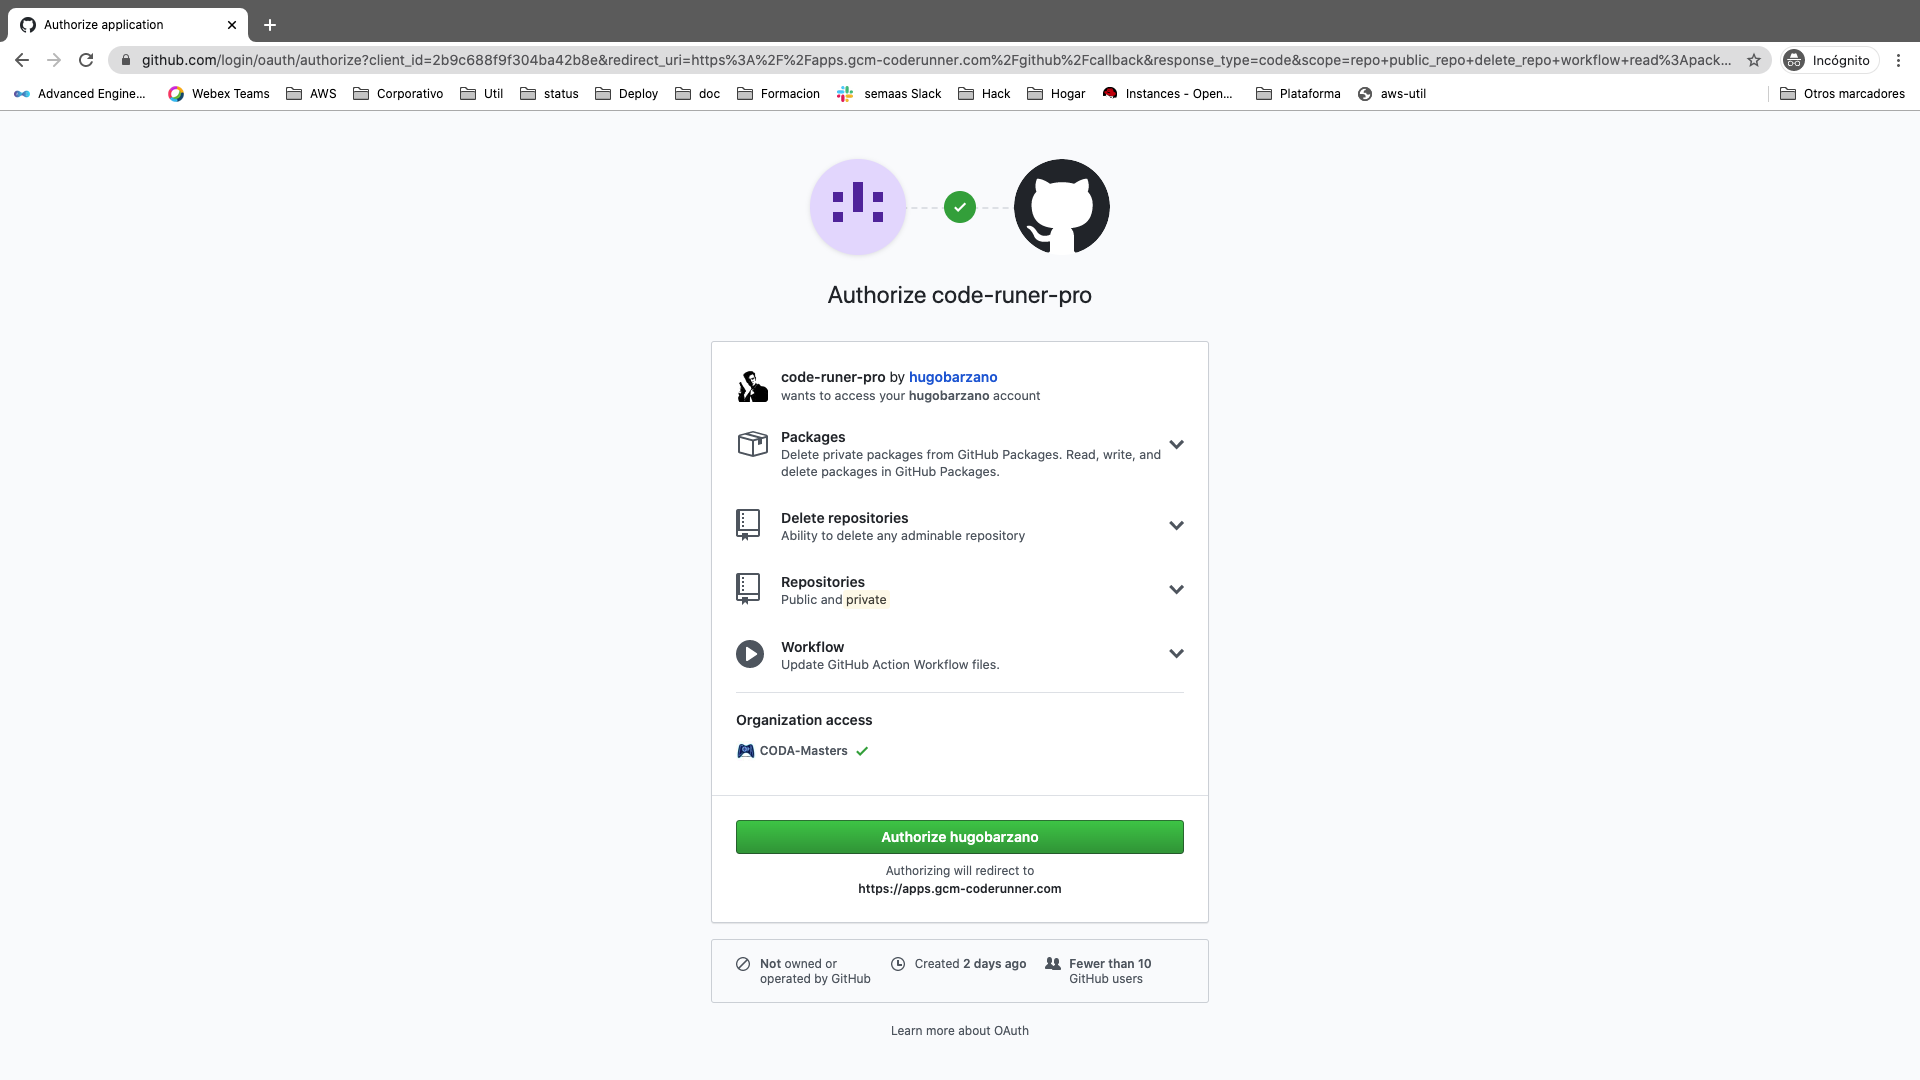
\includegraphics[scale=0.2]{imagenes/casouso/3.png}
\caption{  Autenticación y Autorización: Autorización }
\end{figure}

La autorización consiste en conceder permisos al sistema para realizar operaciones en nombre del usuario. Haciendo click en el botón de \textbf{Authorize} se conceden permisos para gestionar repositorios, gestionar paquetes, crear releases y utilizar flujos de integración continua. 

\begin{figure}[H]
\centering
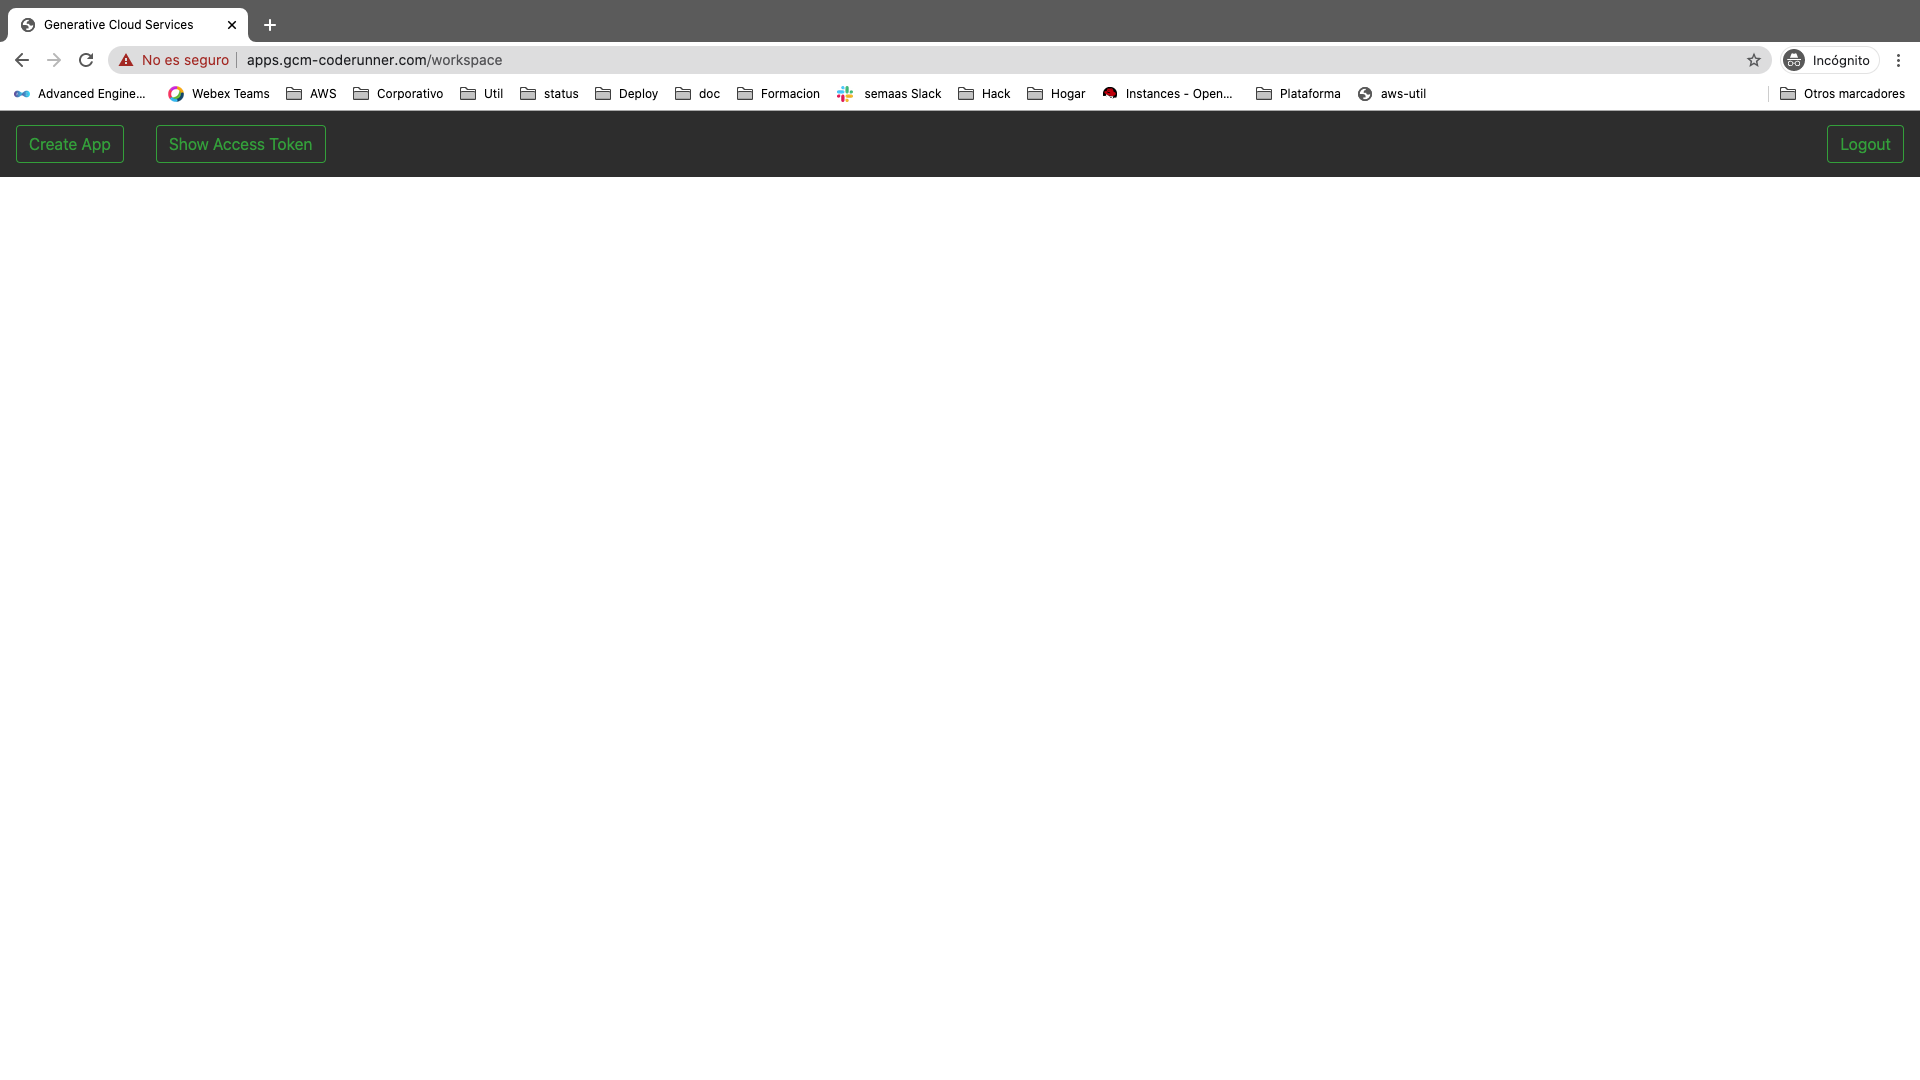
\includegraphics[scale=0.2]{imagenes/casouso/4.png}
\caption{ Autenticación y Autorización: Workspace  }
\end{figure}

Finalmente accede a su \textbf{Workspace} personal que actualmente se encuentra vacío ya que aun no ha creado ninguna aplicación. 

\subsection{Generando Aplicaciones}

Para comenzar a generar aplicaciones, el usuario ha de hacer click en el botón de \textbf{Create App} situado a la izquierda de la barra de navegación superior. El usuario es dirigido al formulario donde especificar el tipo de aplicación que desea generar. 

\begin{figure}[H]
\centering
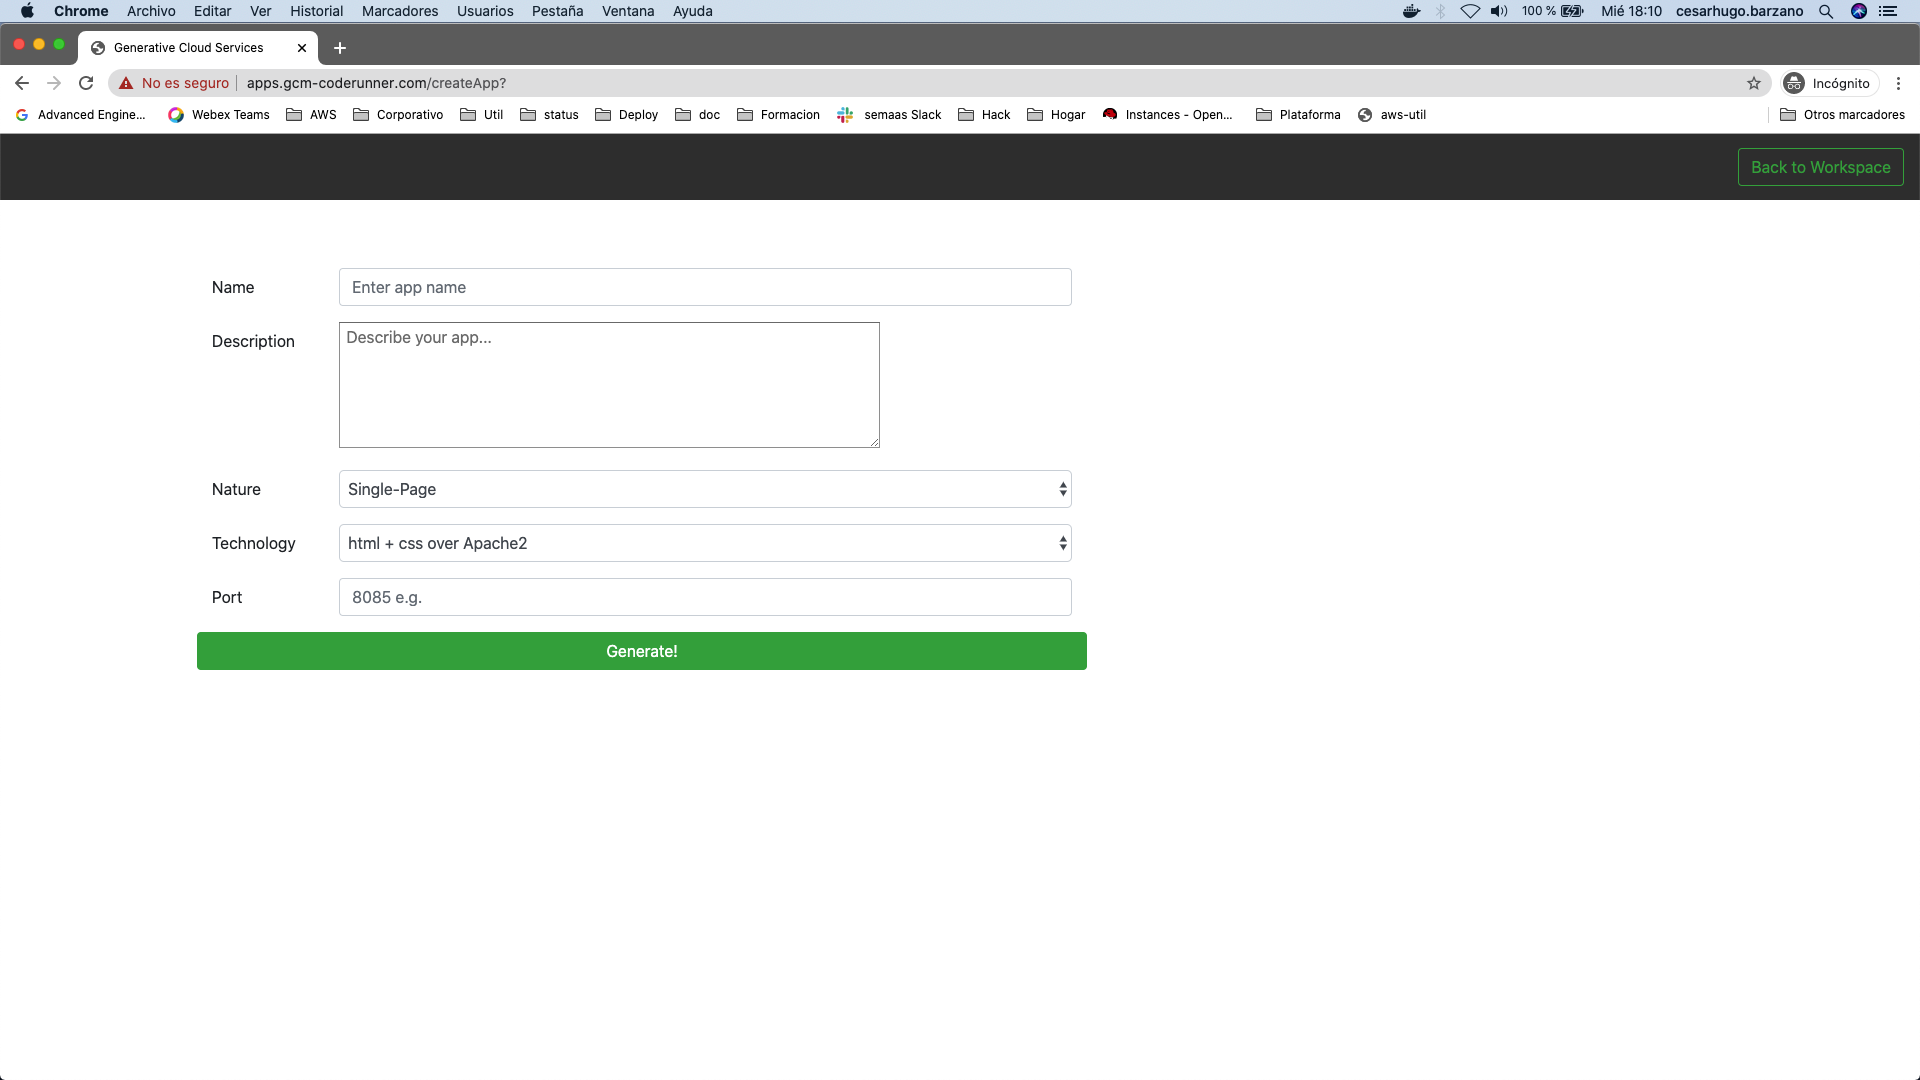
\includegraphics[scale=0.2]{imagenes/casouso/5.png}
\caption{ Generando Aplicaciones: Formulario de Creación  }
\end{figure}

De manera general, la especificación solicita el nombre de la aplicación, una descripción, la naturaleza de la aplicación, la tecnología y el puerto donde se desea desplegar. Las naturalezas soportadas son:

\begin{enumerate}
\item \textbf{ Single-Page: } Aplicaciones web estáticas que se caracterizan por servir contenido estático en una sola pagina con el objetivo de mejorar la experiencia de usuario. 
\item \textbf{ Api-Rest: } Aplicaciones web dinámicas caracterizadas por poseer lógica de negocio y definir interfaces programáticas sobre sistemas software. En algunos casos se incluyen Interfaces Web para ejecutar operaciones sobre estas interfaces.  
\item \textbf{ Data-Service:} Servicios cloud que ofrecen acceso a datos bajo demanda de los usuarios. 
\item \textbf{ DevOps-Service: } Servicios cloud orientados al desarrollo y operación de sistemas software. 
\end{enumerate}

\begin{figure}[H]
\centering
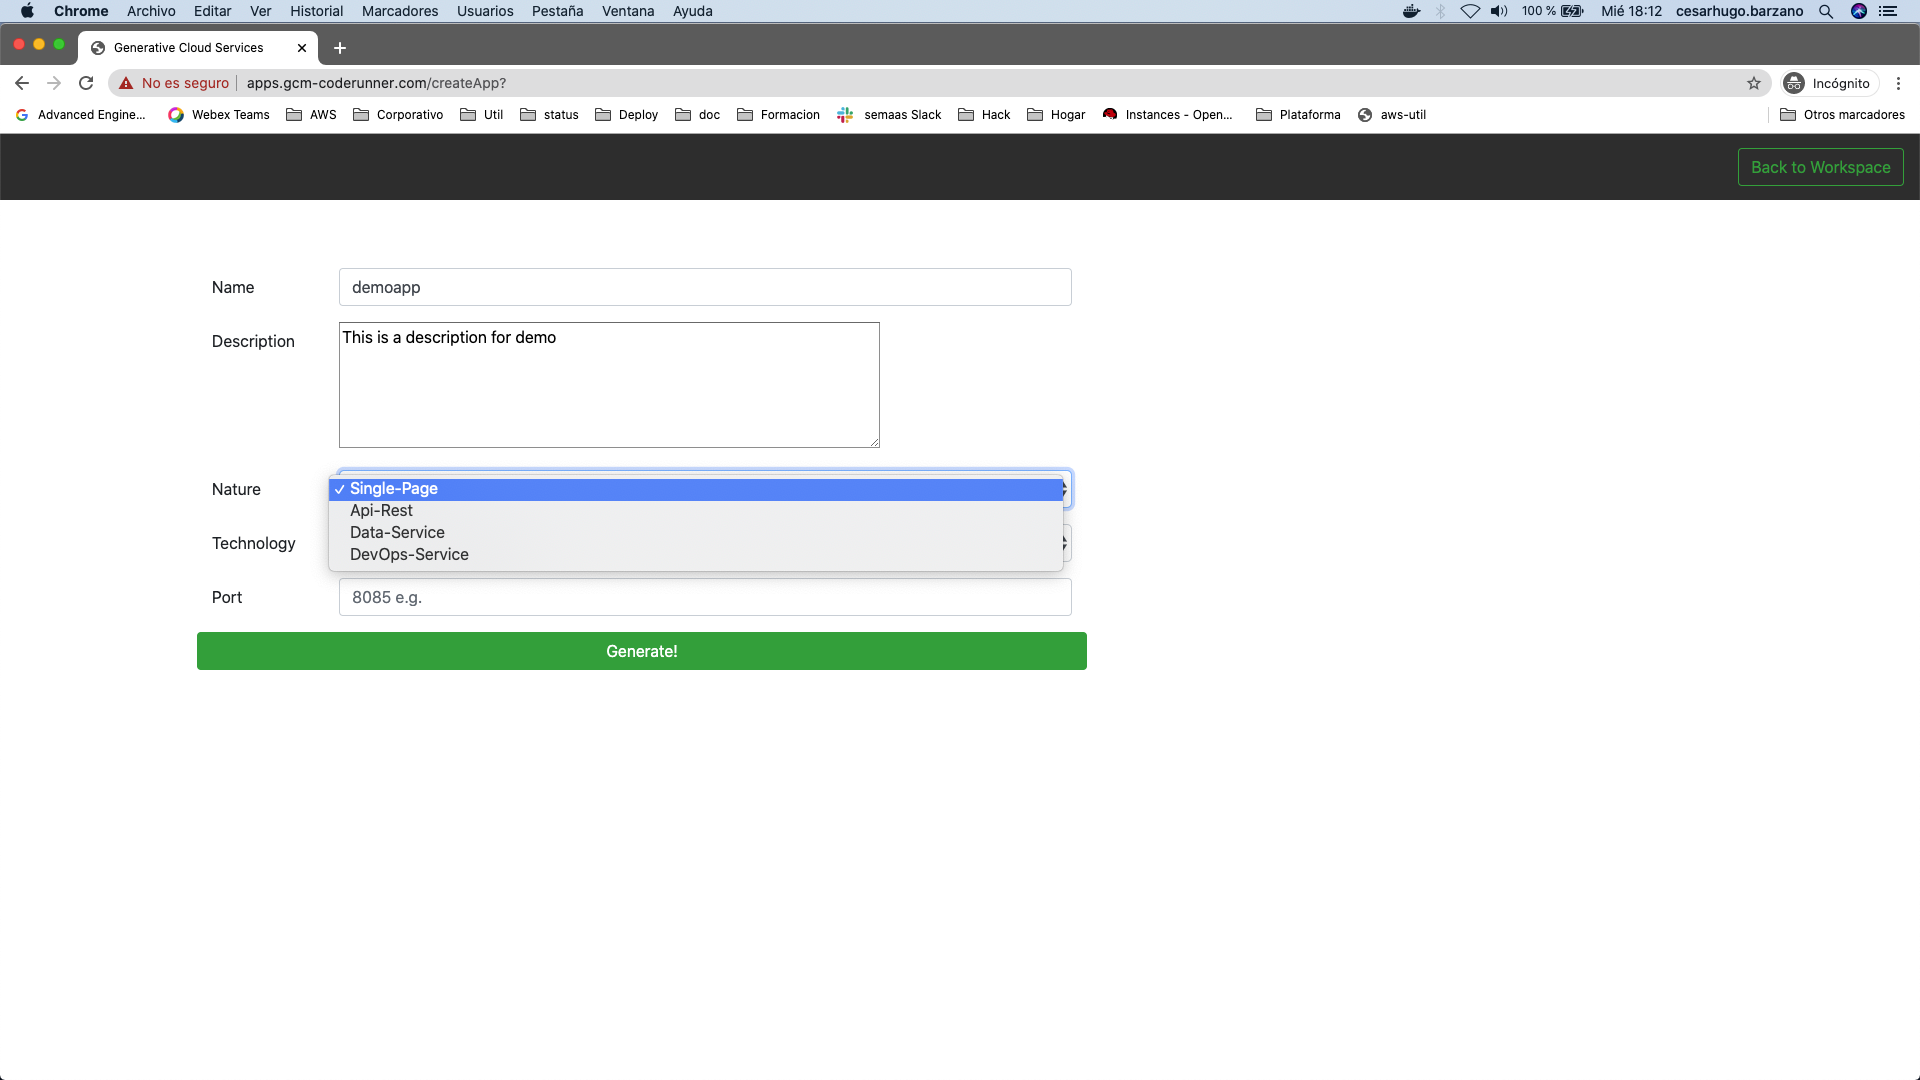
\includegraphics[scale=0.2]{imagenes/casouso/6.png}
\caption{  Generando Aplicaciones: Naturalezas  }
\end{figure}
\subsubsection{Single-Page}

Las tecnologías soportadas para este tipo de aplicación son las siguientes: 

\begin{figure}[H]
\centering
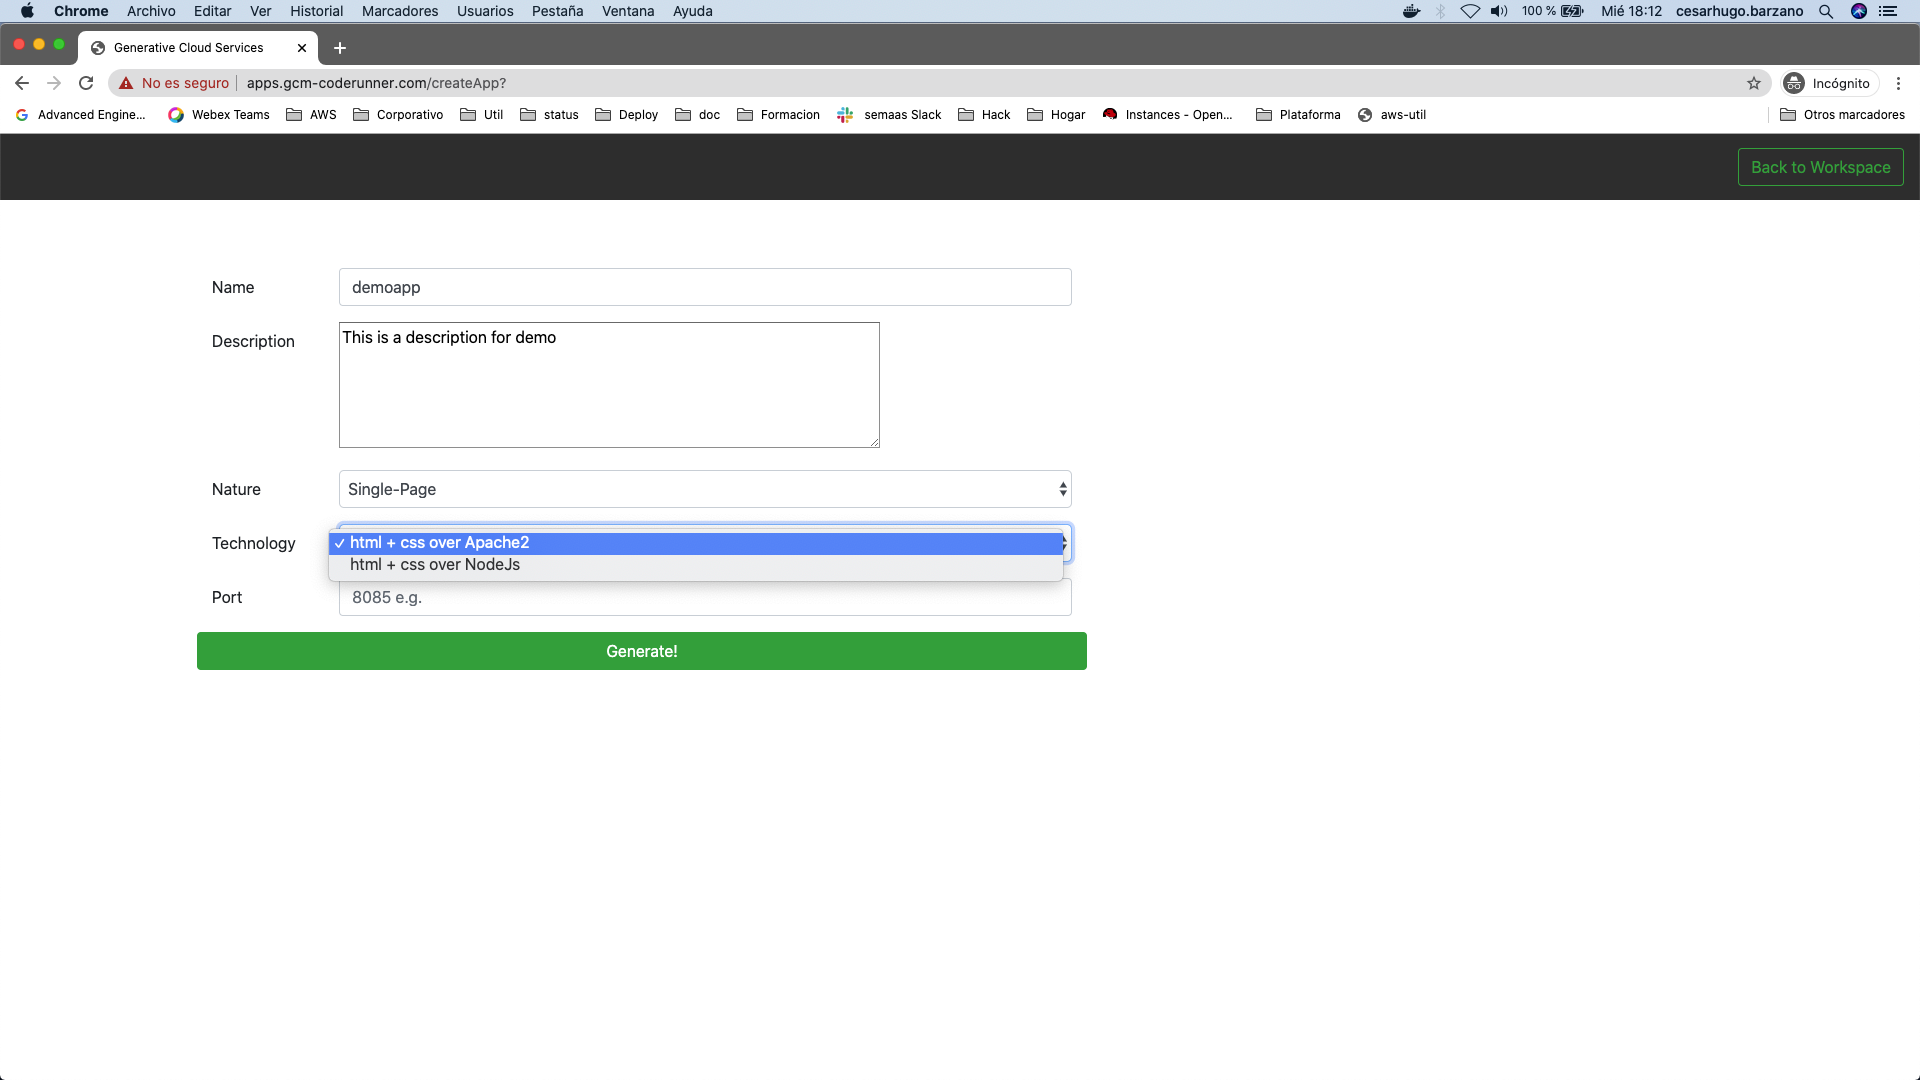
\includegraphics[scale=0.2]{imagenes/casouso/7.png}
\caption{ Generando Aplicaciones: Single-Page   }
\end{figure}

Se establece el puerto de despliegue \textbf{8805} y se hace click sobre el botón \textbf{Generate}.
\begin{figure}[H]
\centering
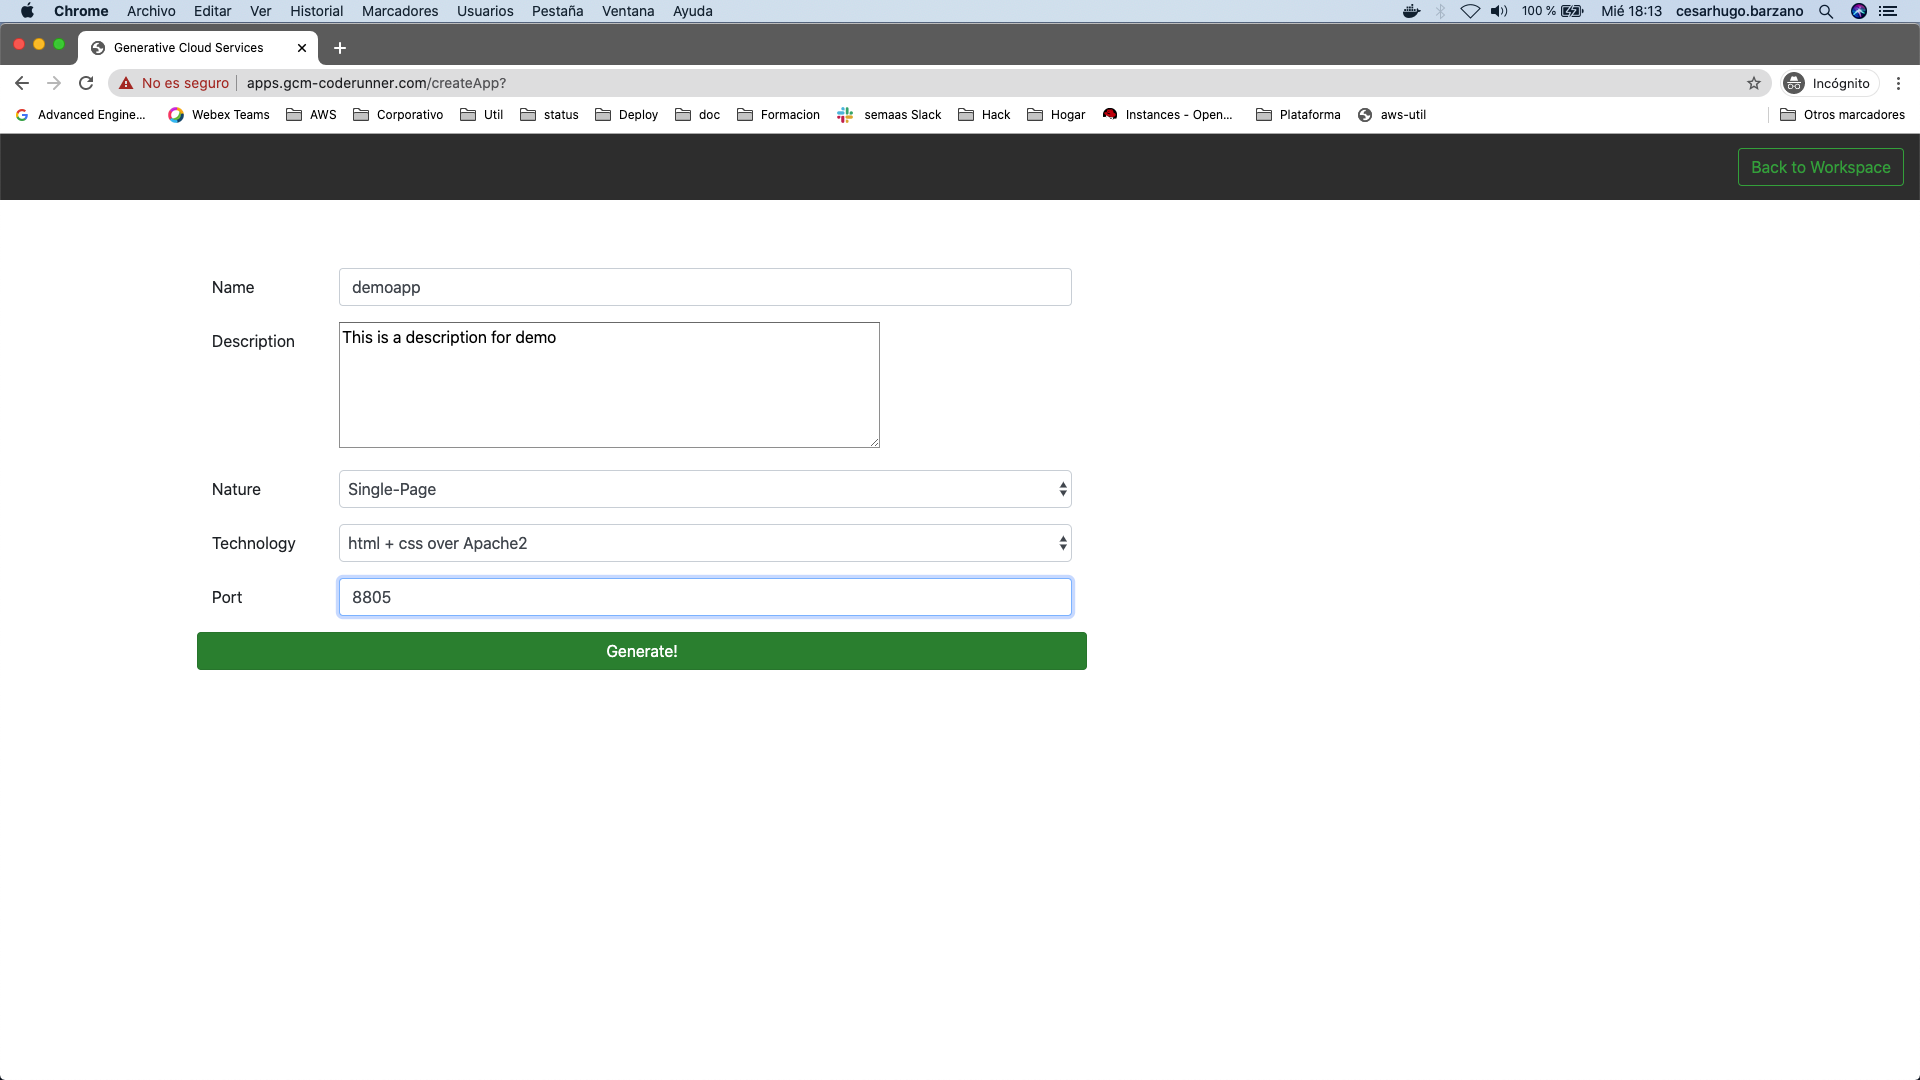
\includegraphics[scale=0.2]{imagenes/casouso/8.png}
\caption{  Generando Aplicaciones: Single-Page  }
\end{figure}

El usuario es redirigido de nuevo al \textbf{Workspace} y la aplicación comienza a ser generada. 

\begin{figure}[H]
\centering
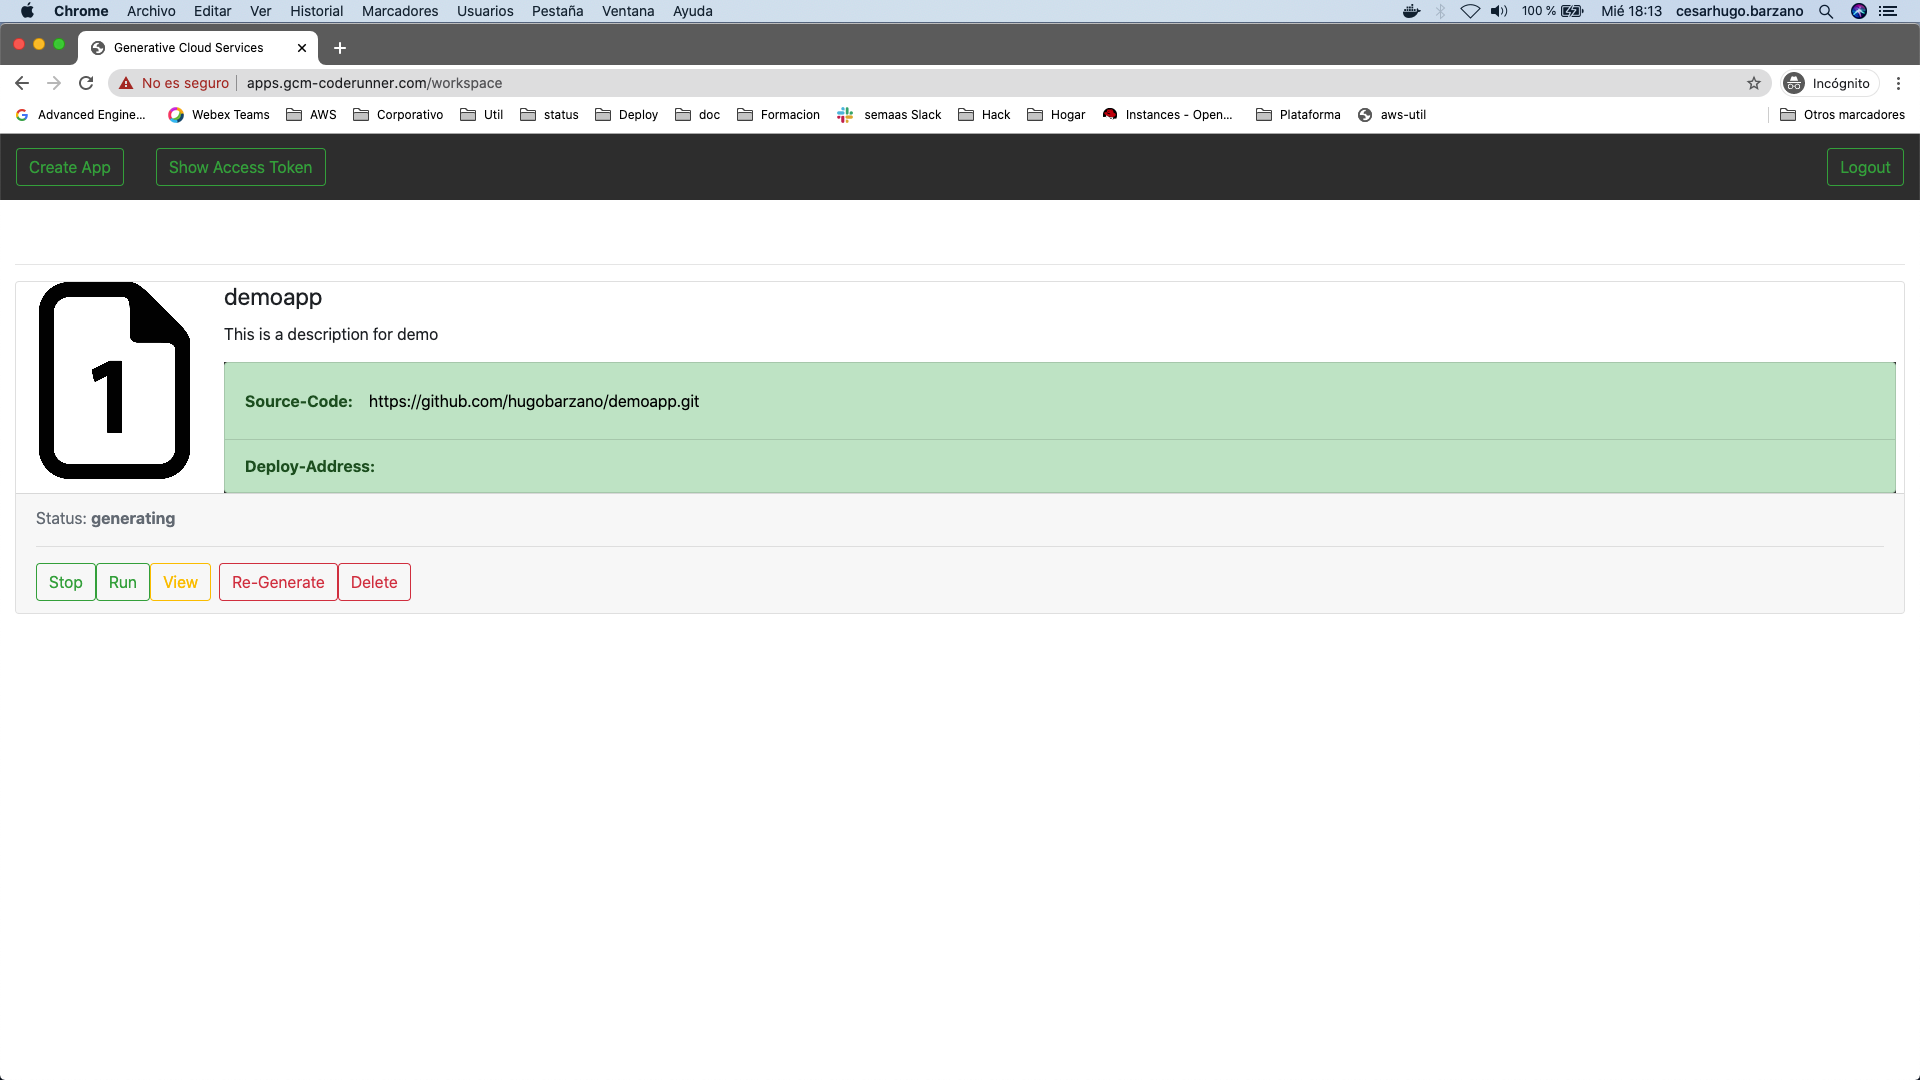
\includegraphics[scale=0.2]{imagenes/casouso/9.png}
\caption{ Generando Aplicaciones: Single-Page  }
\end{figure}


Toda la producción de código fuente es albergada en un repositorio de código creado en la cuenta del usuario. Haciendo click en el enlace disponible en el apartado \textbf{Source-Code}
el usuario puede consultar dicho código fuente. 

\begin{figure}[H]
\centering
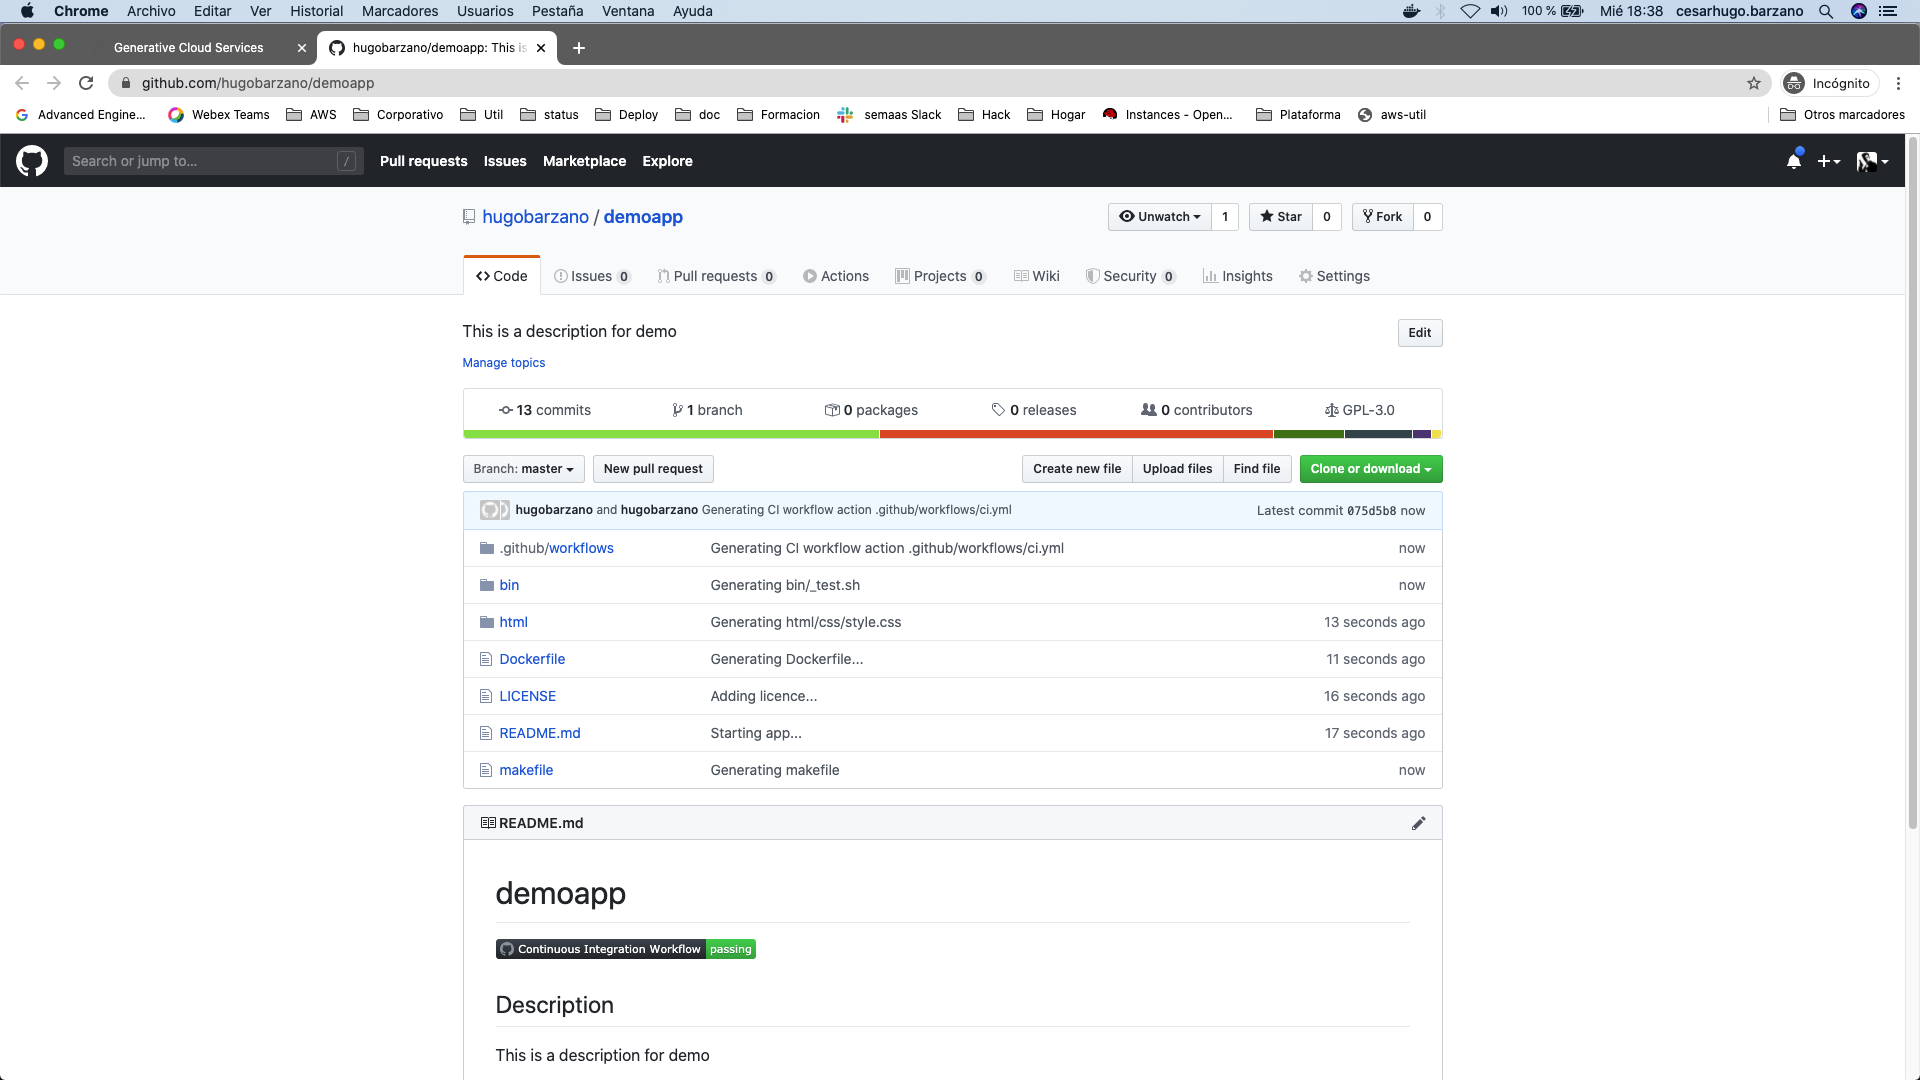
\includegraphics[scale=0.2]{imagenes/casouso/10.png}
\caption{  Generando Aplicaciones: Single-Page Repositorio }
\end{figure}

Cuando el proceso de generación finaliza, comienza el ciclo de integración continua, el cual es definido como una \textbf{Github Action}.

\begin{figure}[H]
\centering
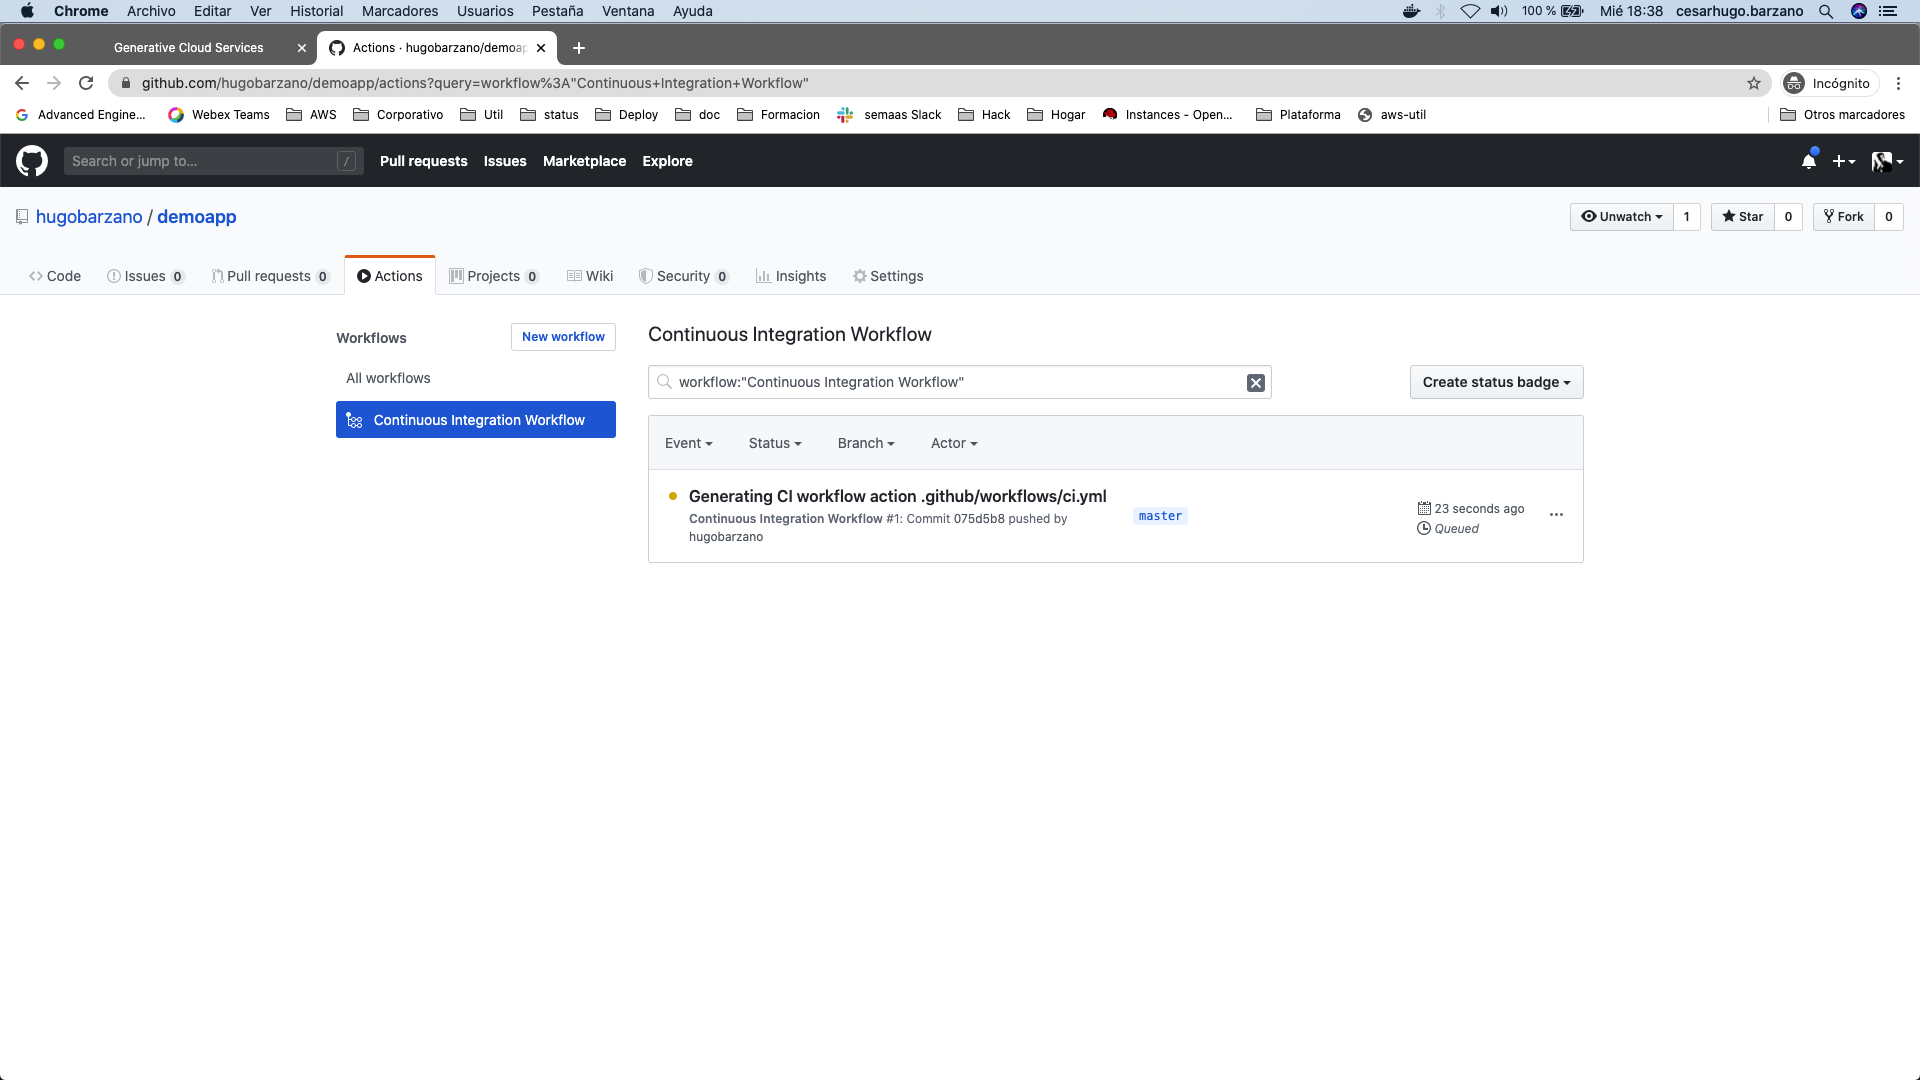
\includegraphics[scale=0.2]{imagenes/casouso/11.png}
\caption{  Generando Aplicaciones: Single-Page CI }
\end{figure}

Si el usuario vuelve al \textbf{Workspace} puede comprobar que efectivamente el estado de la aplicación es \textbf{building}. 
\begin{figure}[H]
\centering
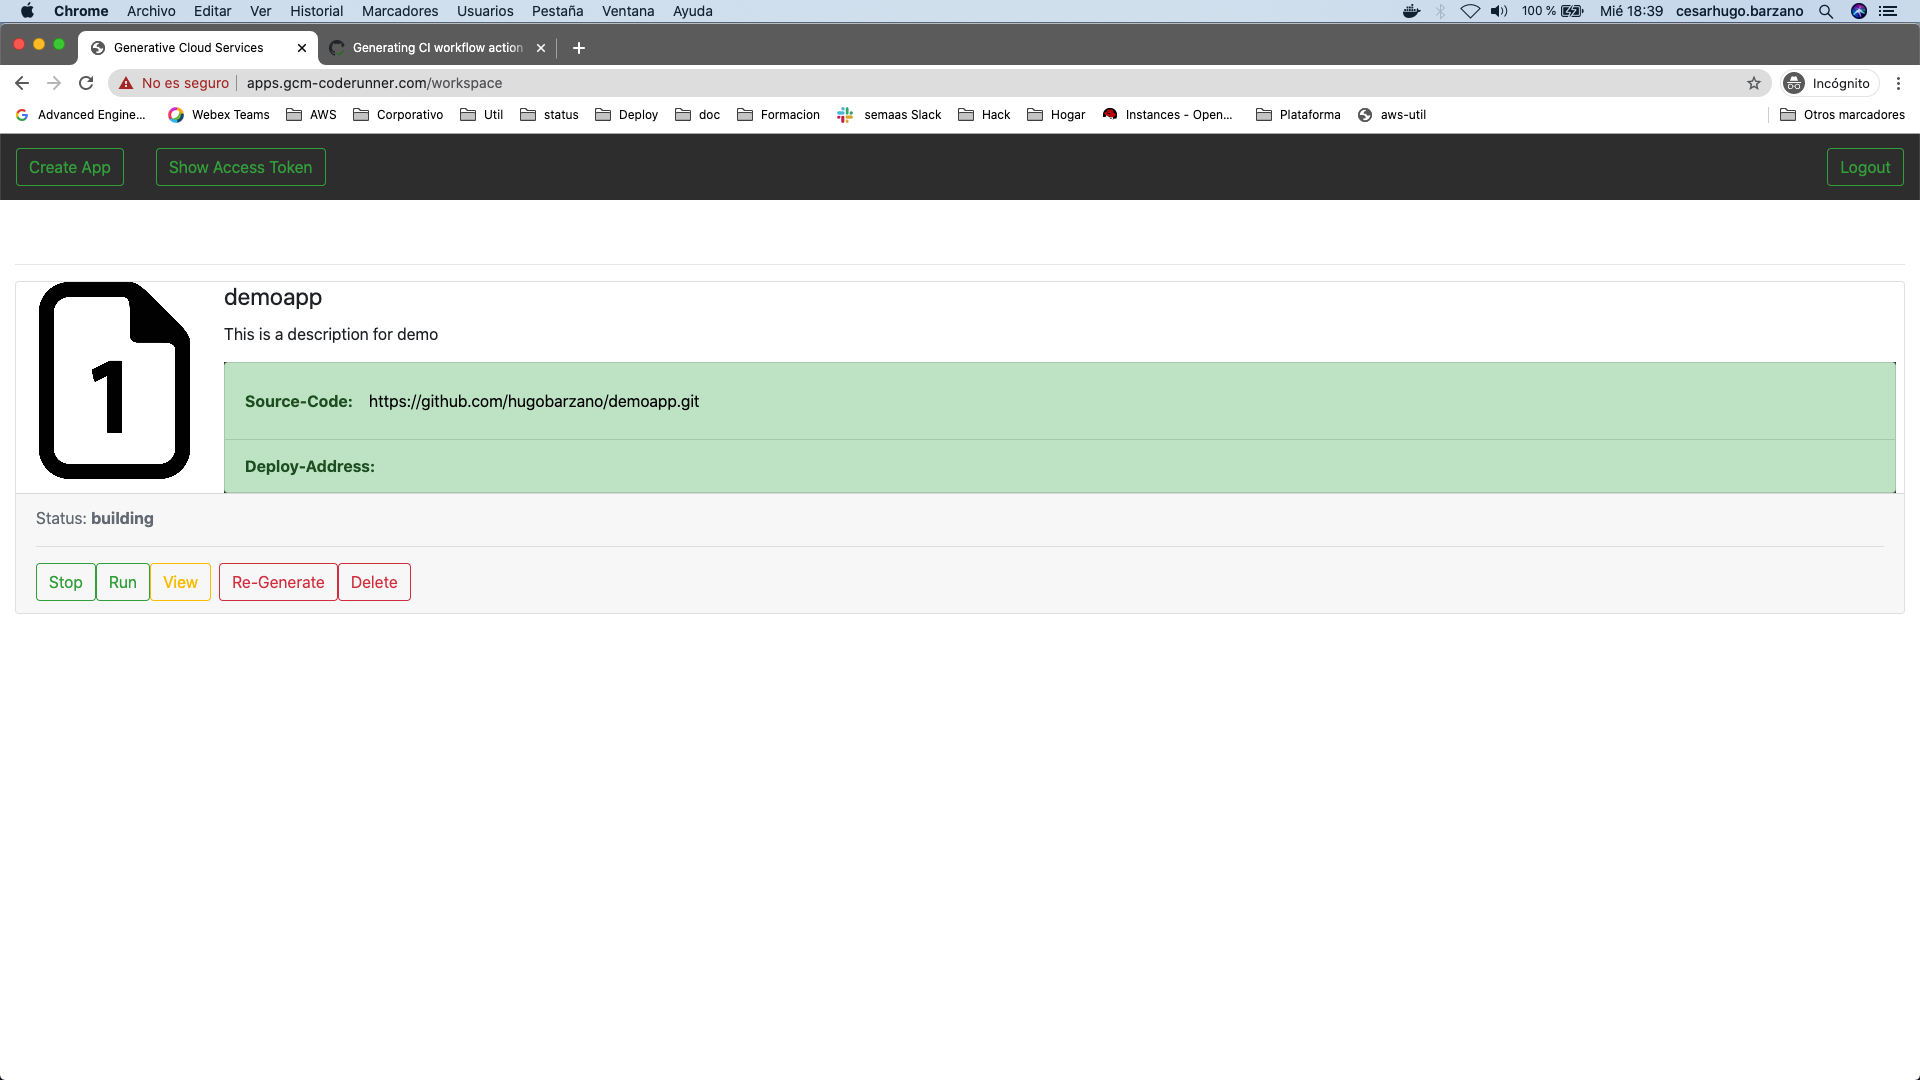
\includegraphics[scale=0.2]{imagenes/casouso/12.png}
\caption{ Generando Aplicaciones: Single-Page Compilación  }
\end{figure}


Este flujo de integración continua se divide en una serie de fases en las que se ejecutan las pruebas unitarias, se compila la aplicación generada y finalmente se empaqueta el artefacto:

\begin{figure}[H]
\centering
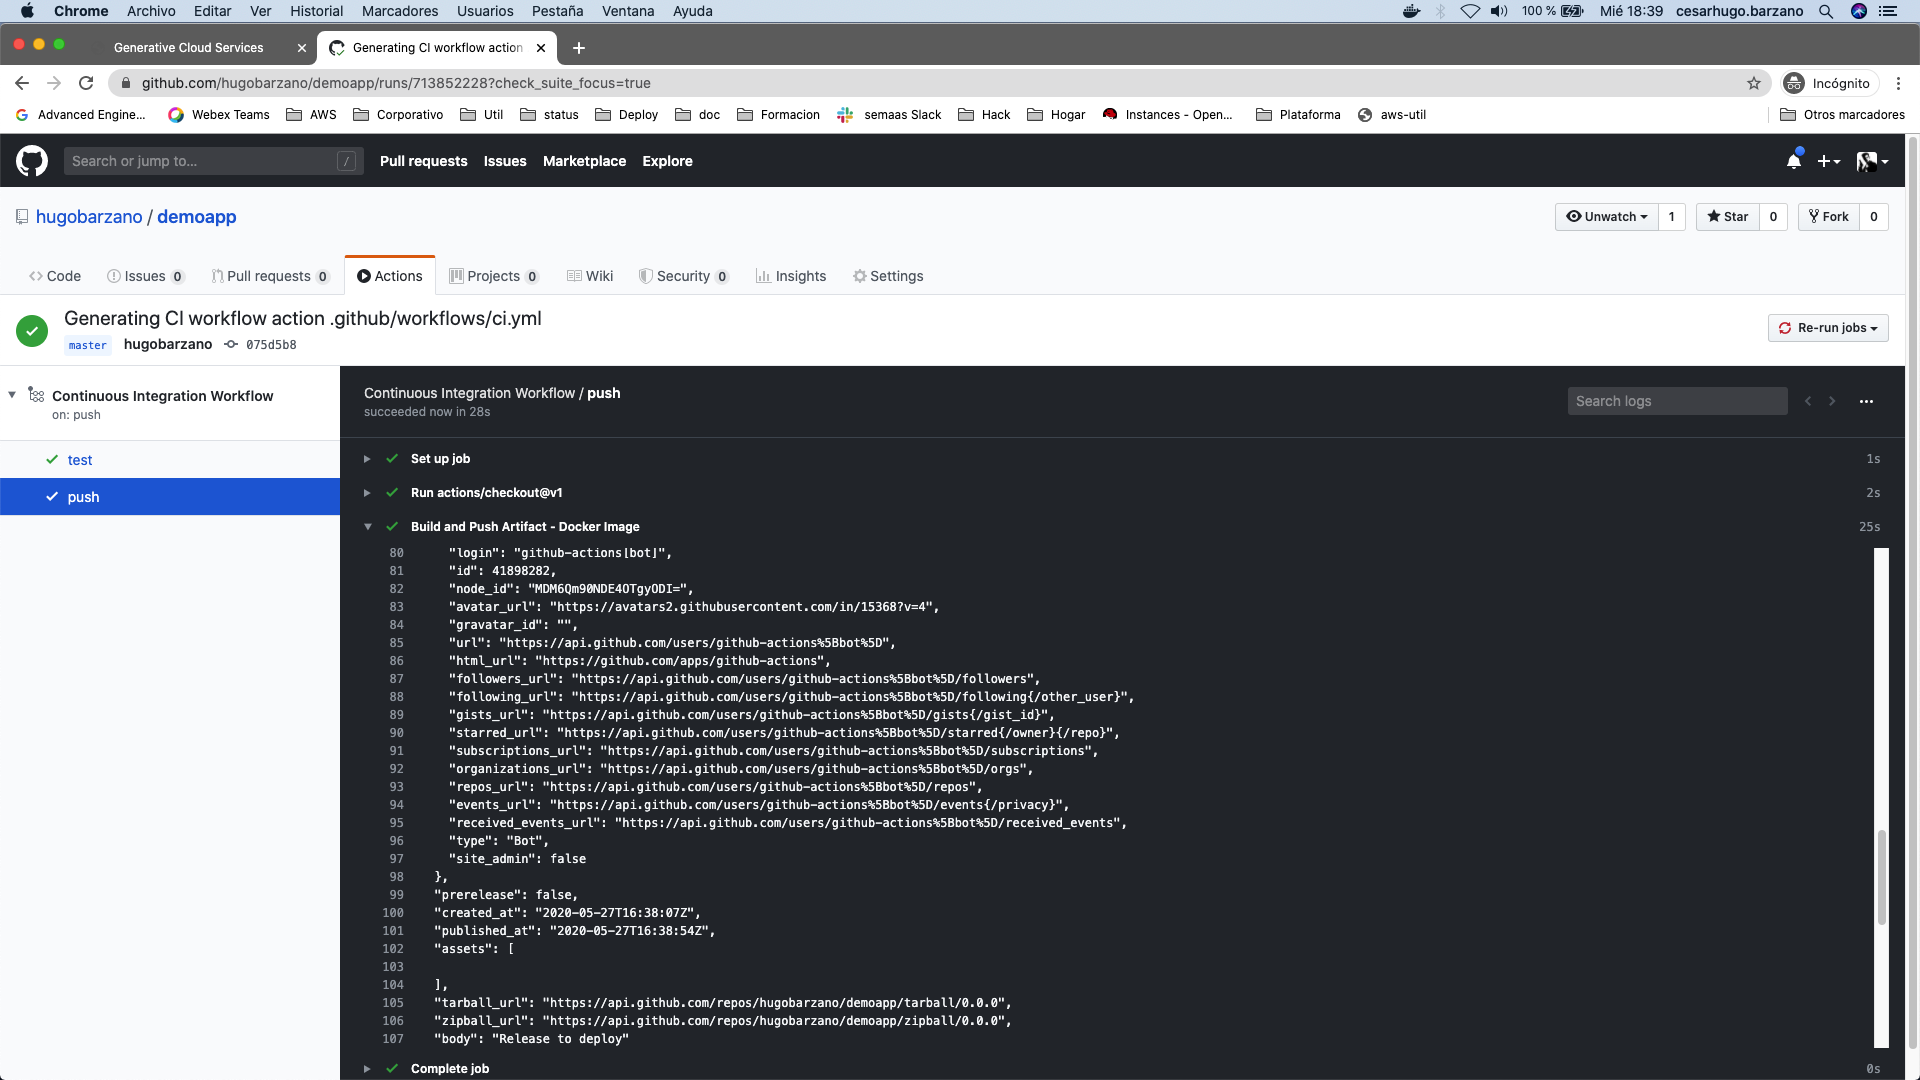
\includegraphics[scale=0.2]{imagenes/casouso/13.png}
\caption{ Generando Aplicaciones: Single-Page CI Completado  }
\end{figure}

El resultado de este flujo es por una parte un Release que identifica de manera única al estado del código fuente y por otra el artefacto que se va a desplegar: 

\begin{figure}[H]
\centering
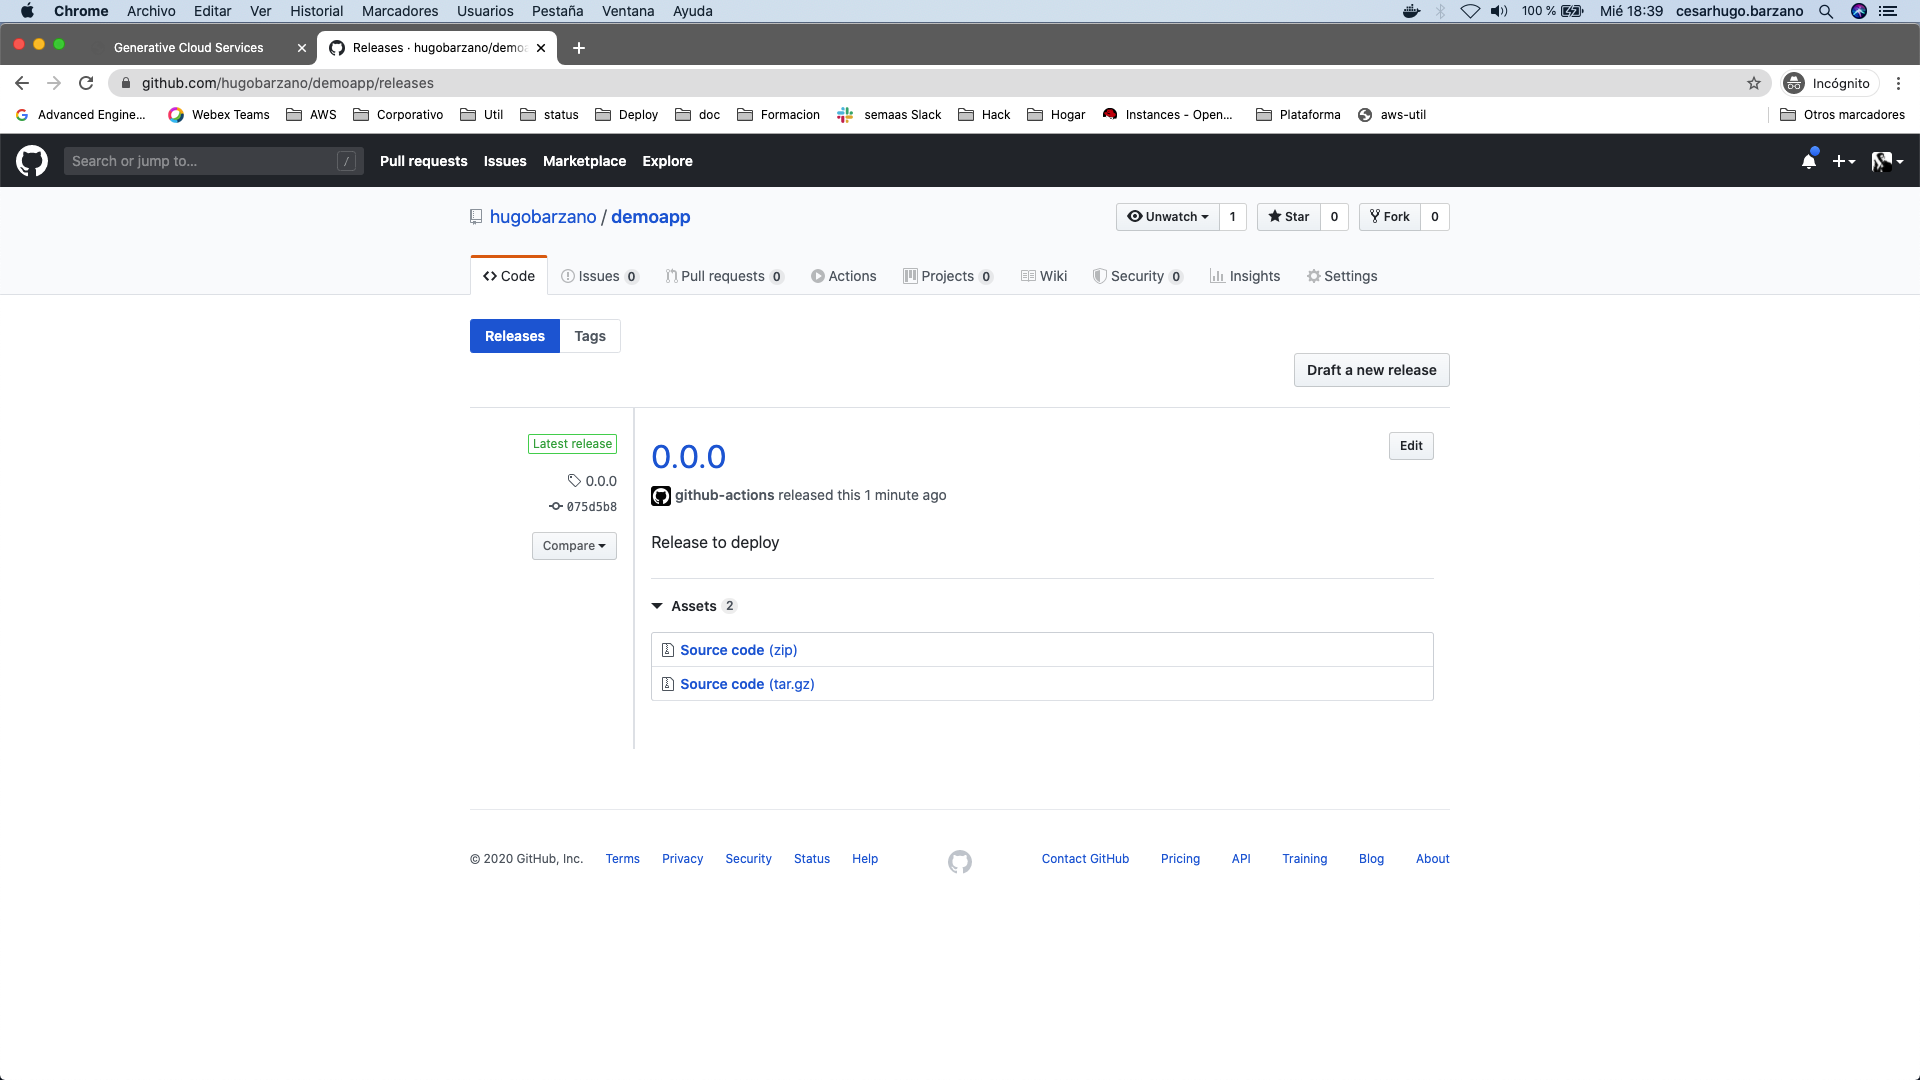
\includegraphics[scale=0.2]{imagenes/casouso/14.png}
\caption{ Generando Aplicaciones: Single-Page Release  }
\end{figure}

\begin{figure}[H]
\centering
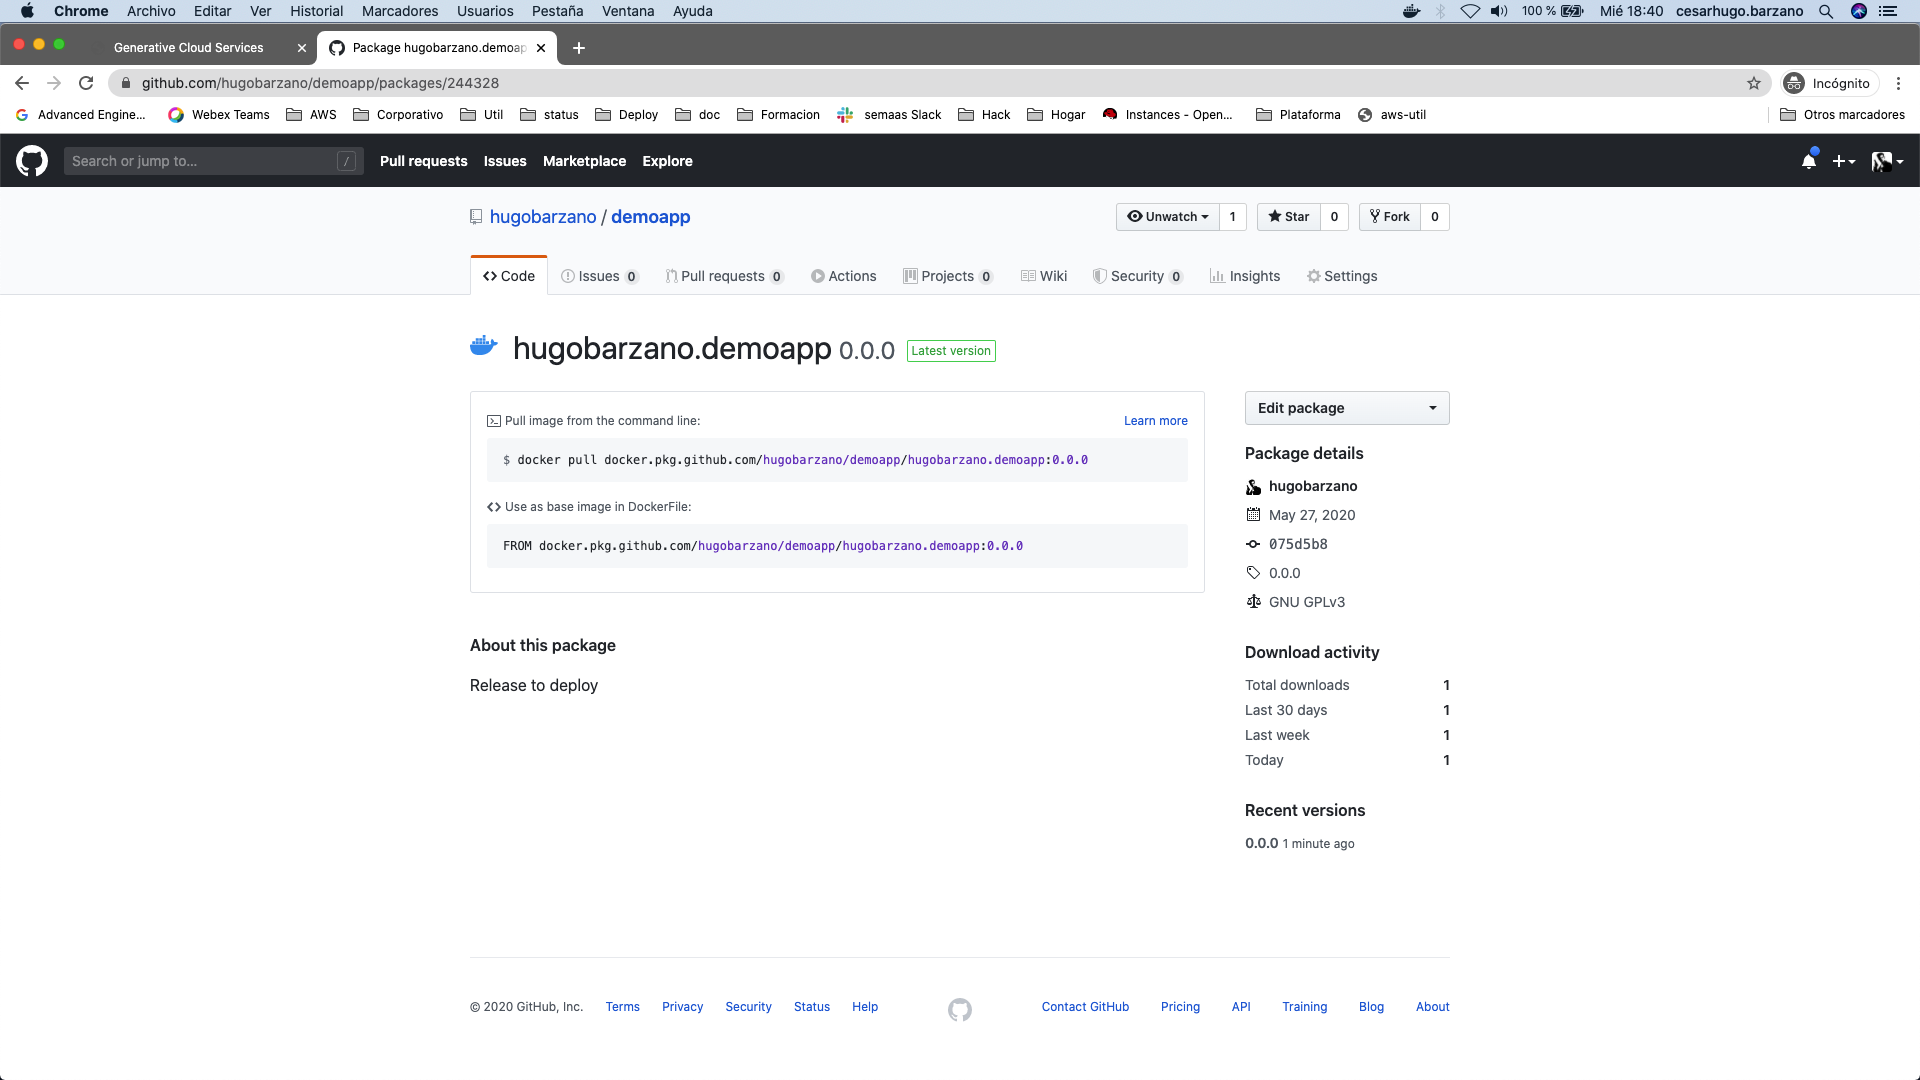
\includegraphics[scale=0.2]{imagenes/casouso/15.png}
\caption{  Generando Aplicaciones: Single-Page Artefacto}
\end{figure}

Si el usuario vuelve a poner el foco en su \textbf{Workspace} encuentra de nuevo un cambio de estado, la aplicación esta \textbf{running}, es decir, ha sido desplegada. 
\begin{figure}[H]
\centering
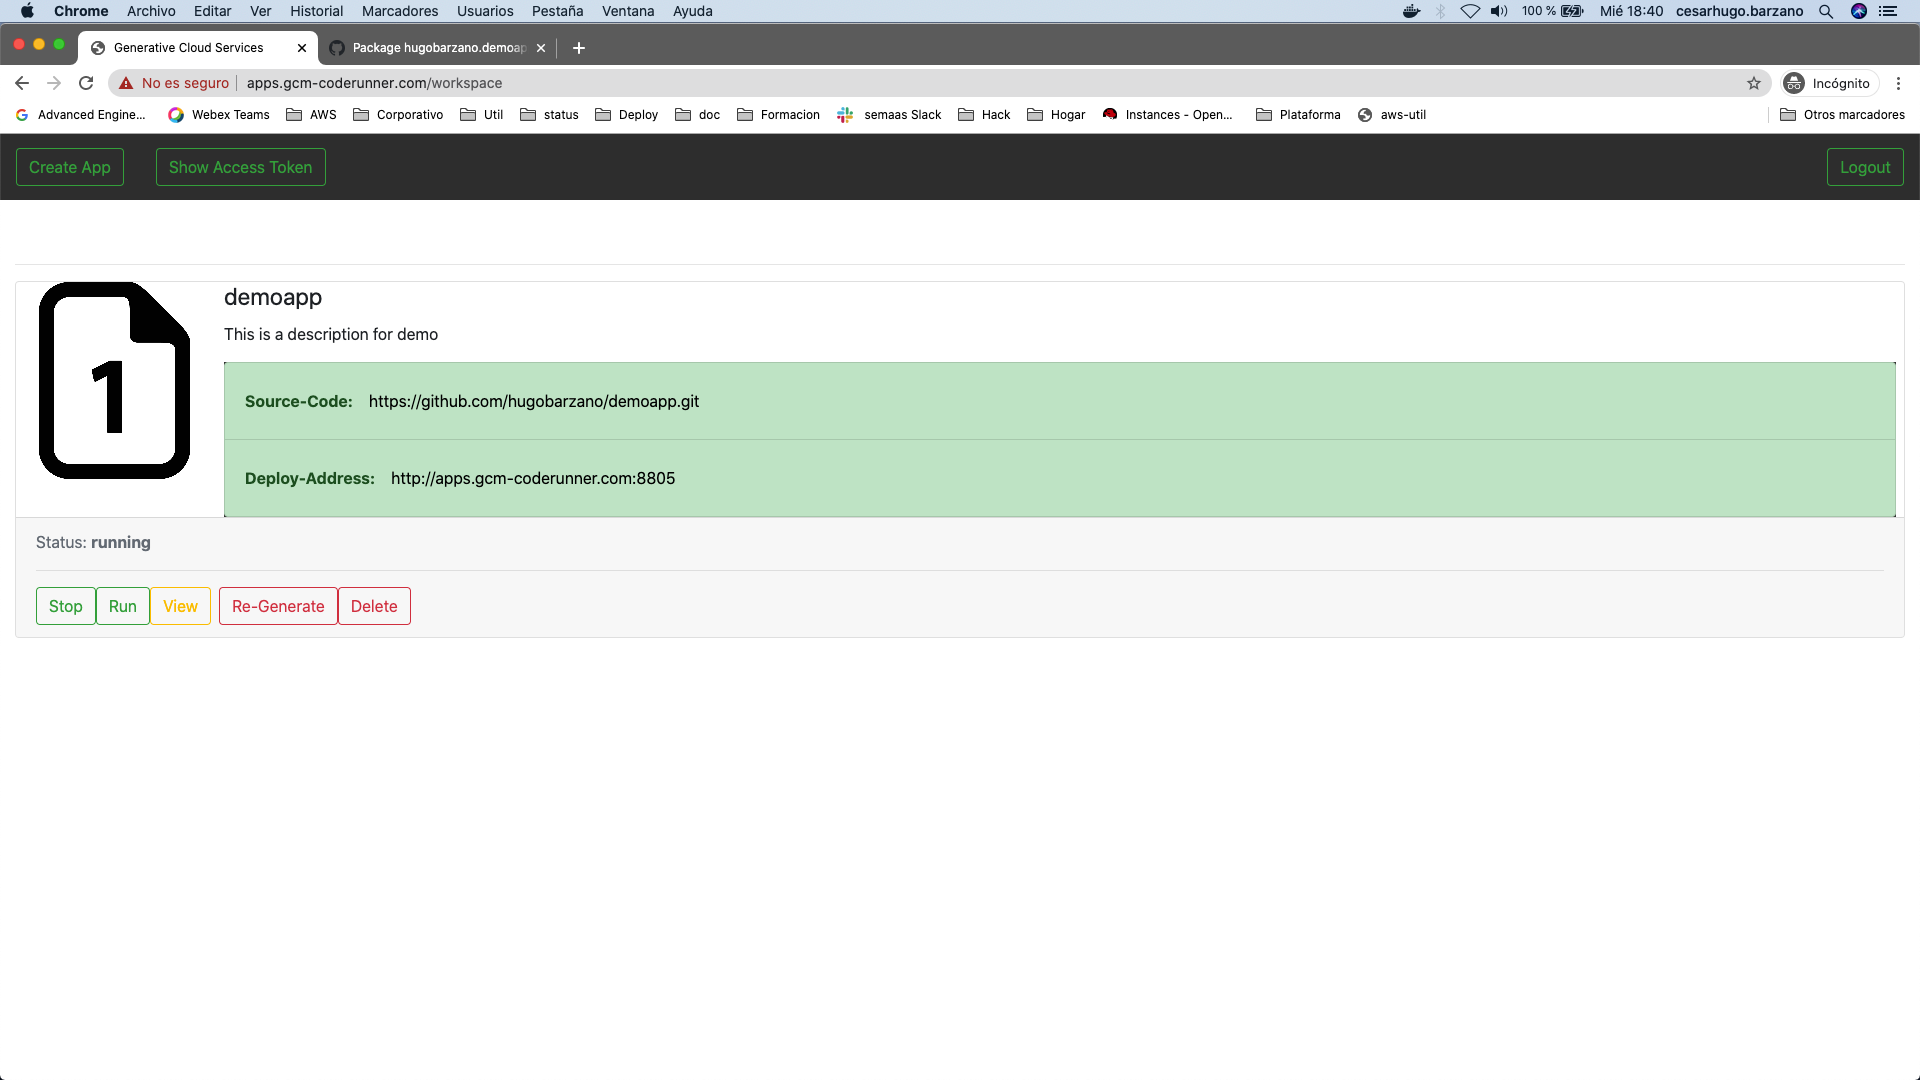
\includegraphics[scale=0.2]{imagenes/casouso/16.png}
\caption{   Generando Aplicaciones: Single-Page Desplegada }
\end{figure}

 Haciendo uso del enlace disponible en la entrada \textbf{Deploy-Address} puede consumirla a través de Internet. 

\begin{figure}[H]
\centering
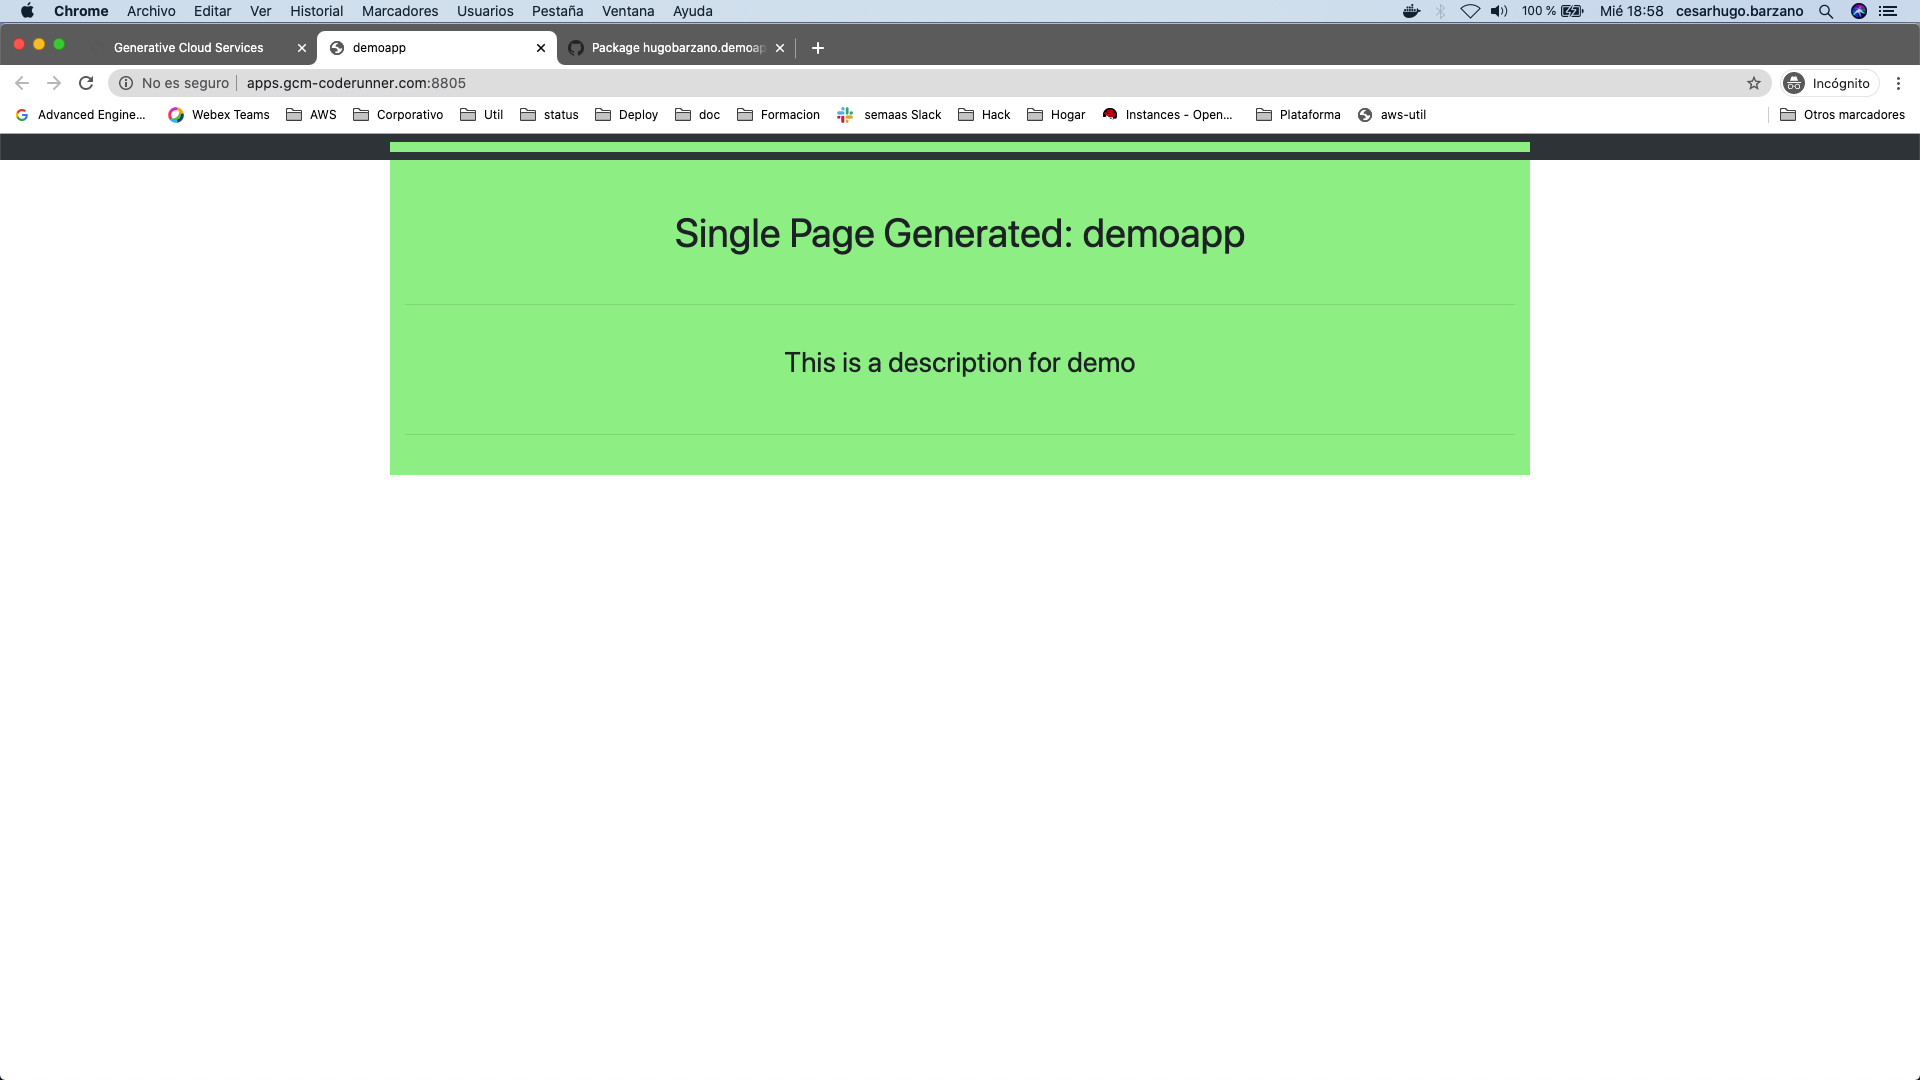
\includegraphics[scale=0.2]{imagenes/casouso/17.png}
\caption{  Generando Aplicaciones: Single-Page Consultada }
\end{figure}

\subsubsection{Api-Rest}

Las tecnologías soportadas para este tipo de aplicación son las siguientes: 

\begin{figure}[H]
\centering
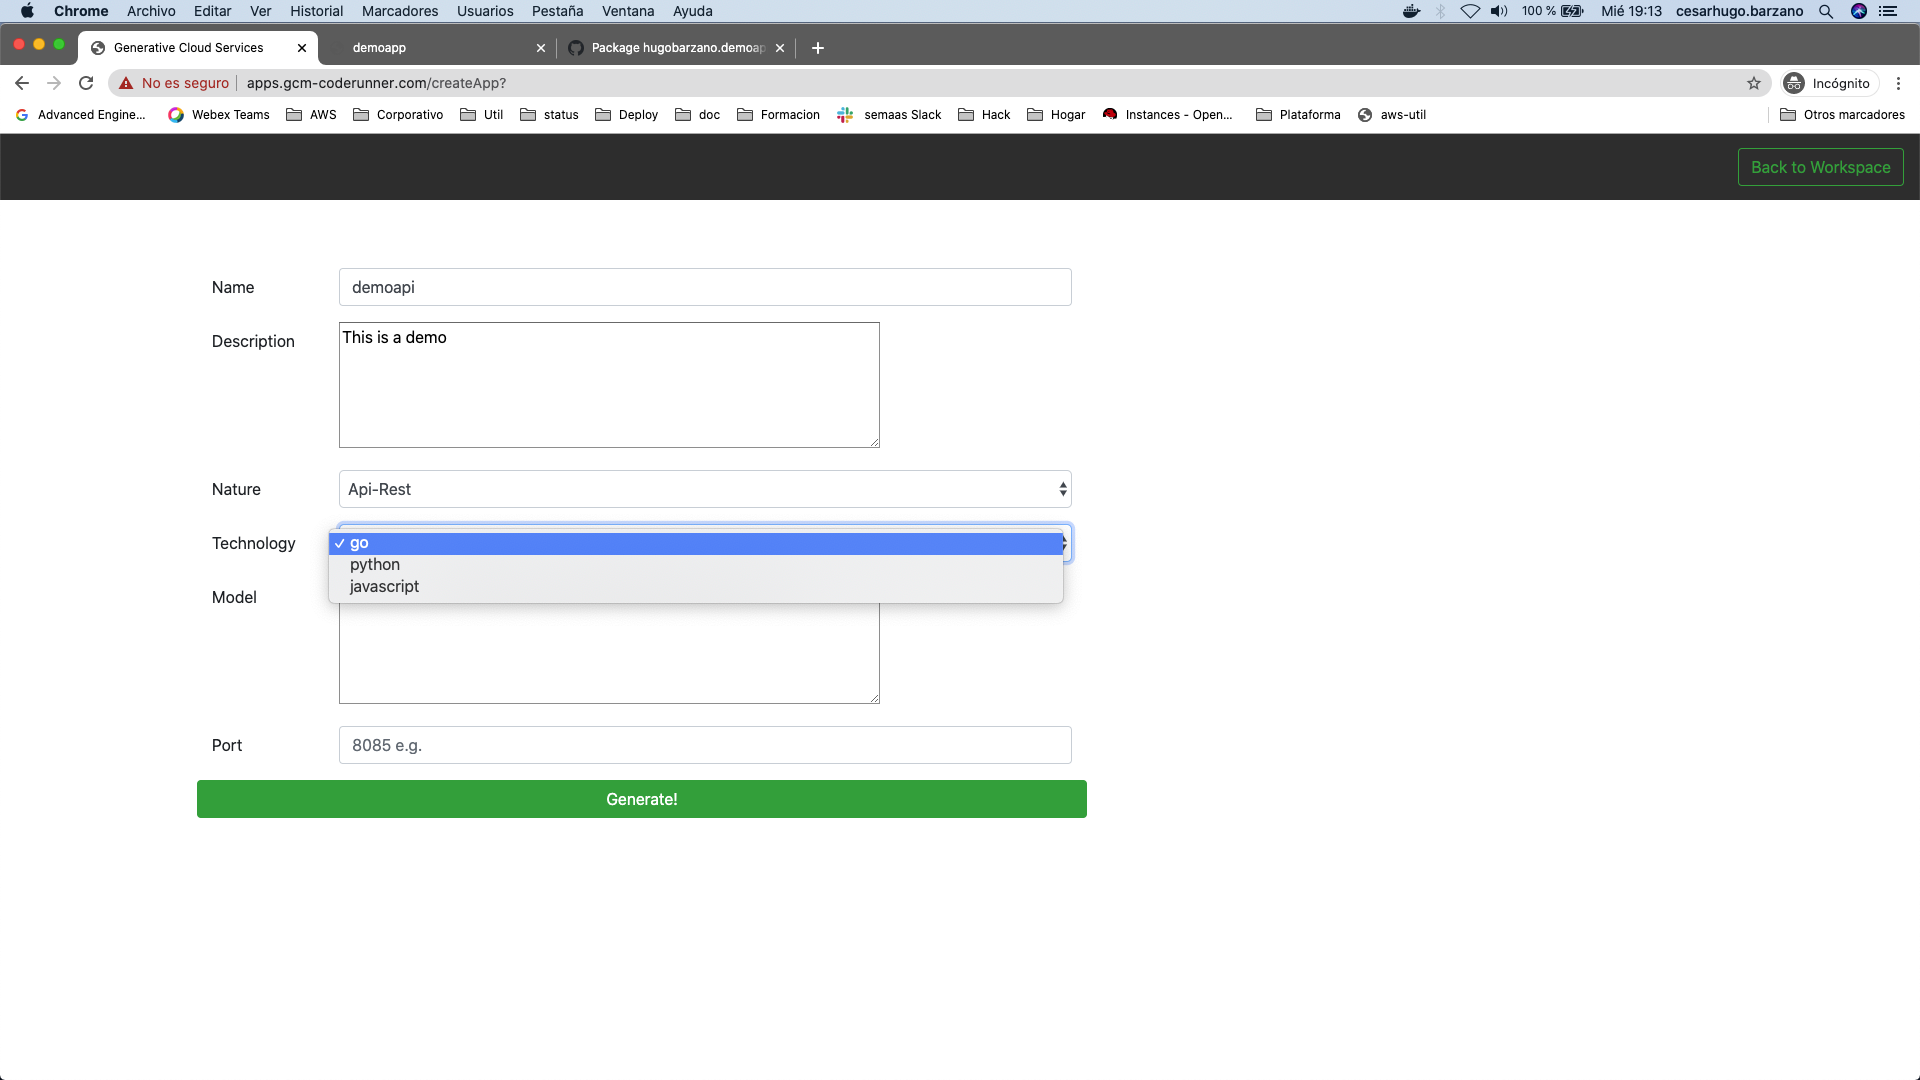
\includegraphics[scale=0.2]{imagenes/casouso/18.png}
\caption{  Generando Aplicaciones: Api-Rest Tecnología }
\end{figure}

Una de las principales características de las aplicaciones base REST es que soportan lógica de negocio para realizar operaciones sobre un modelo de datos. Por ello, para esta naturaleza la especificación requiere de un modelo de datos en formato JSON:

\begin{figure}[H]
\centering
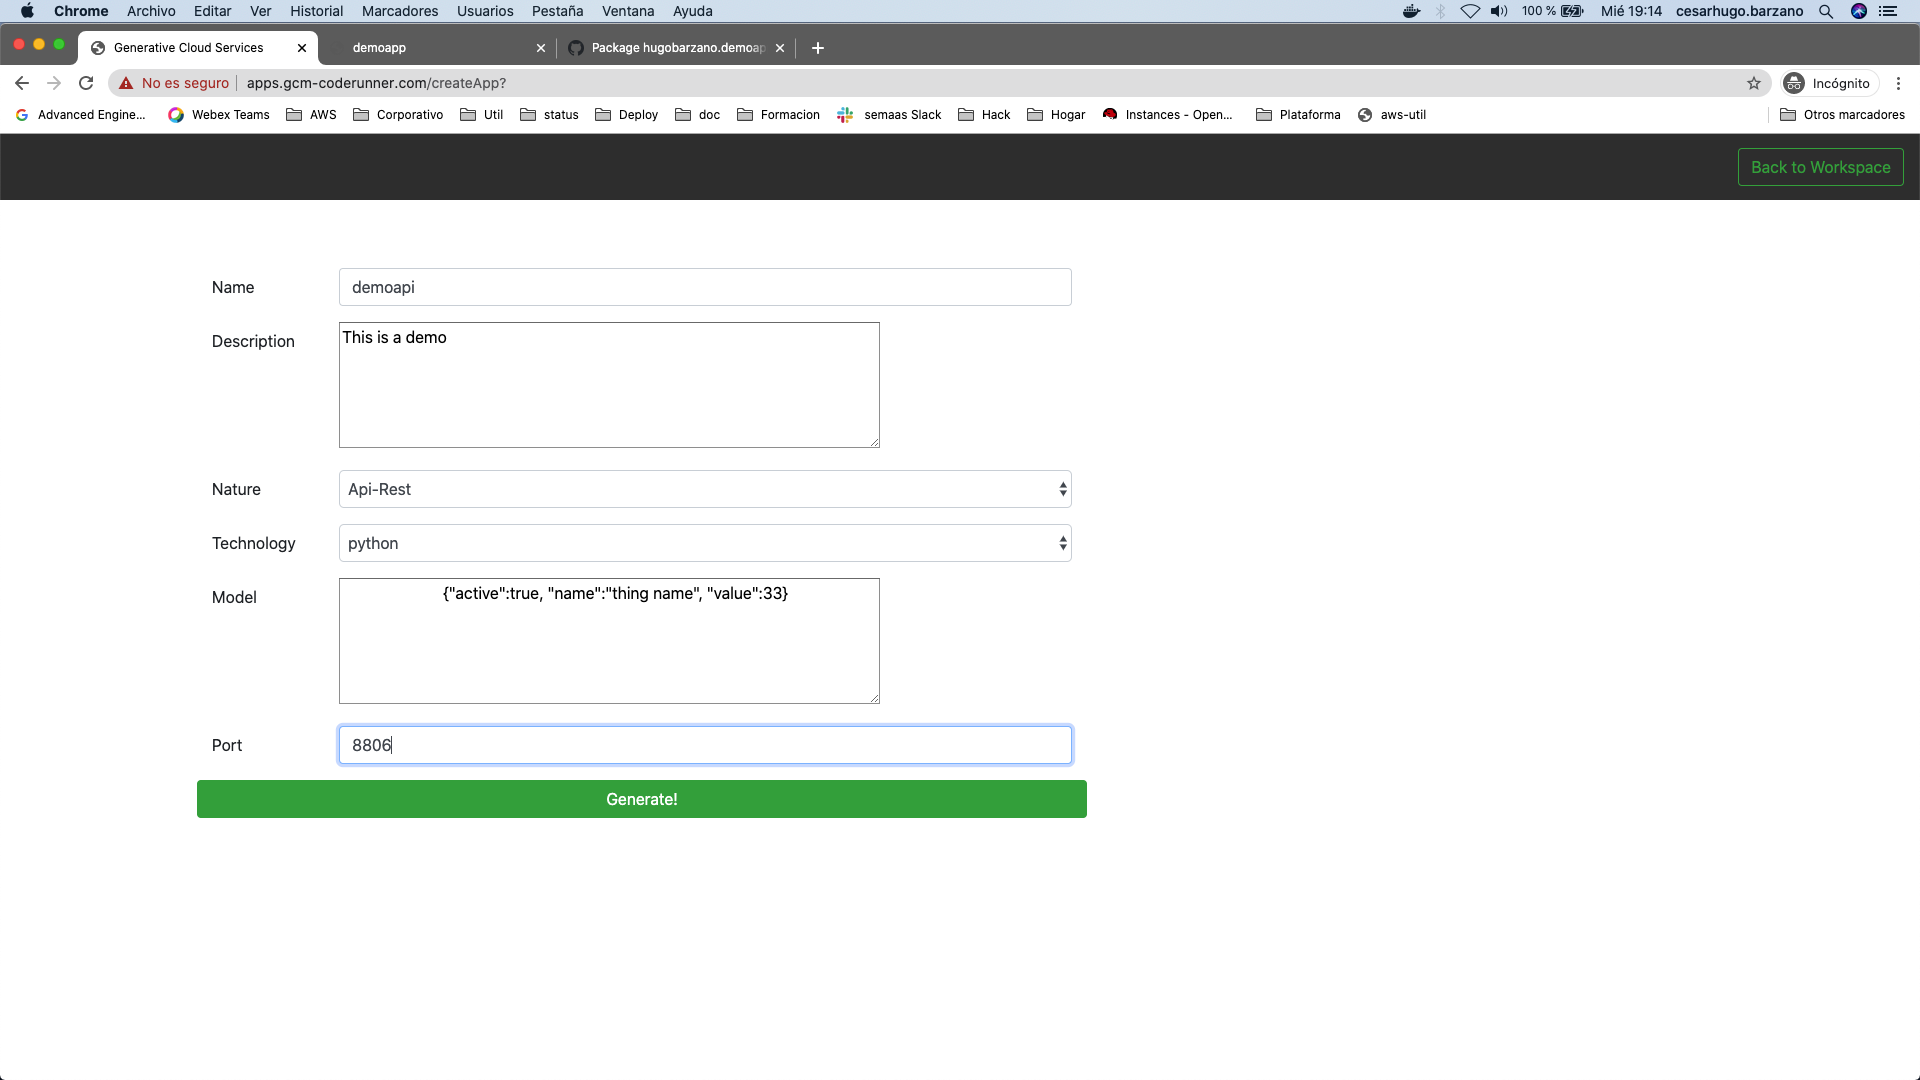
\includegraphics[scale=0.2]{imagenes/casouso/19.png}
\caption{  Generando Aplicaciones: Api-Rest Modelo de Datos  }
\end{figure}

\subsubsection{Data-Service}

Las tecnologías soportadas para este tipo de aplicación son las siguientes: 

\begin{figure}[H]
\centering
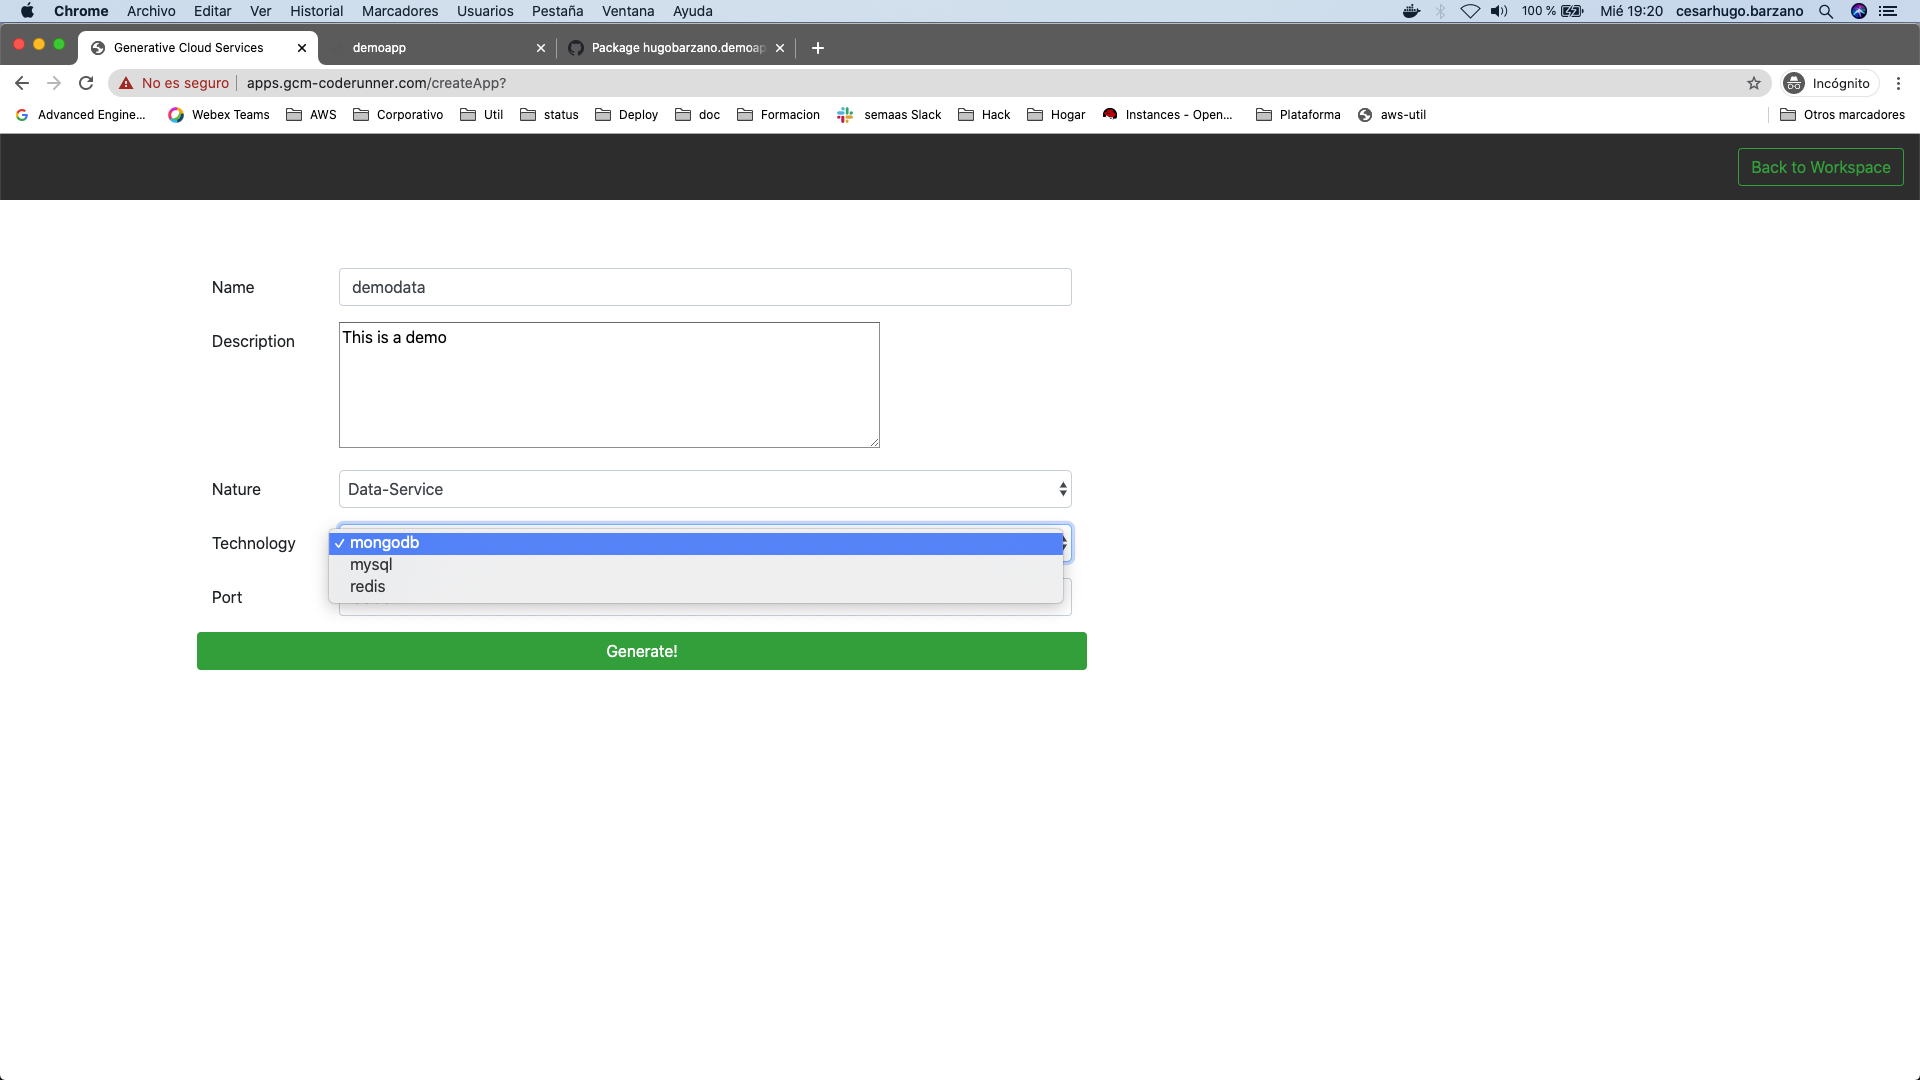
\includegraphics[scale=0.2]{imagenes/casouso/20.png}
\caption{  Generando Aplicaciones: Data-Service Tecnología  }
\end{figure}

Esta caracterización abarca principalmente servicios para la persistencia de datos o mecanismo de cache.

\subsubsection{DevOps-Service}

Las tecnologías soportadas para este tipo de aplicación son las siguientes: 

\begin{figure}[H]
\centering
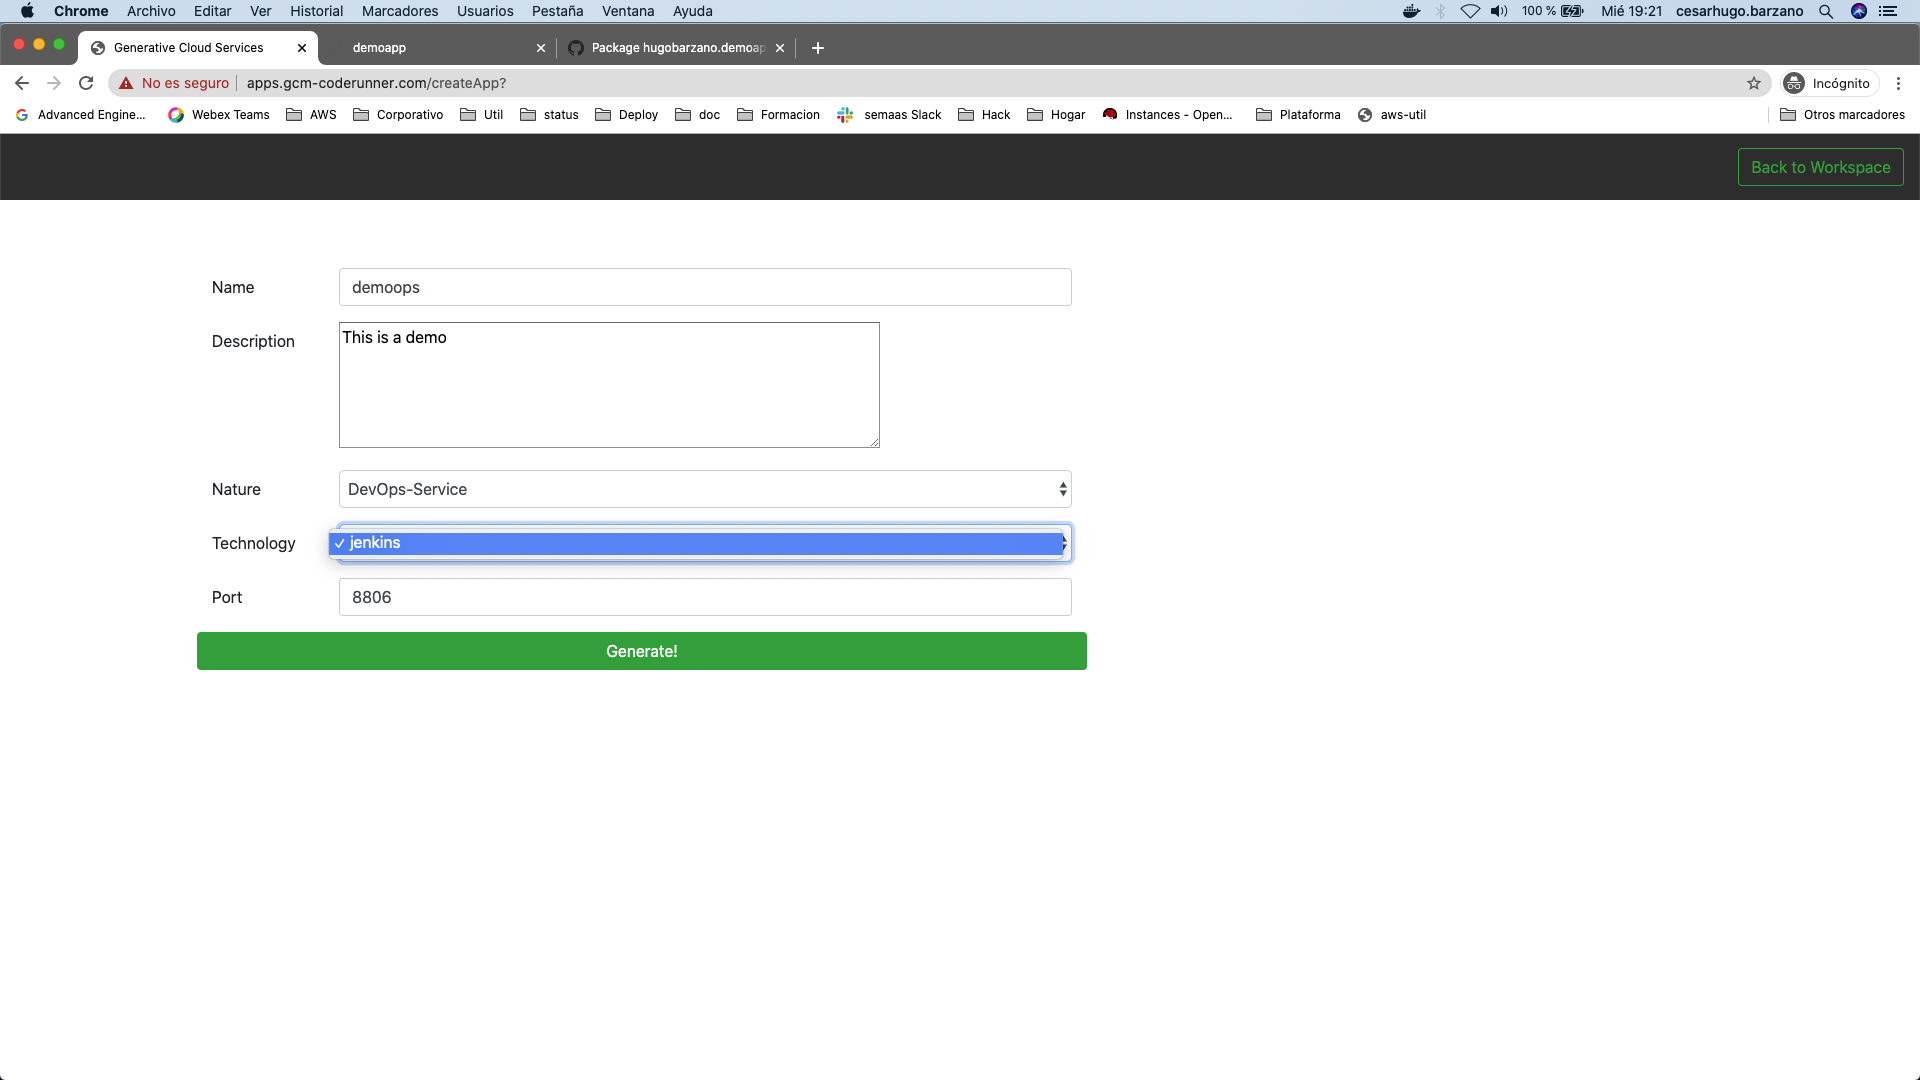
\includegraphics[scale=0.2]{imagenes/casouso/21.png}
\caption{ Generando Aplicaciones: DevOps-Service Tecnología   }
\end{figure}

Presentando por ejemplo un servidor de automatización de tareas como es el caso de Jenkins CI. 

\subsubsection{Workspace}

Una vez generadas las aplicaciones propuestas, el usuario puede navegar entre ellas desde su \textbf{Workspace} . El ciclo de integración continua es similar para todas ellas. 
\begin{figure}[H]
\centering
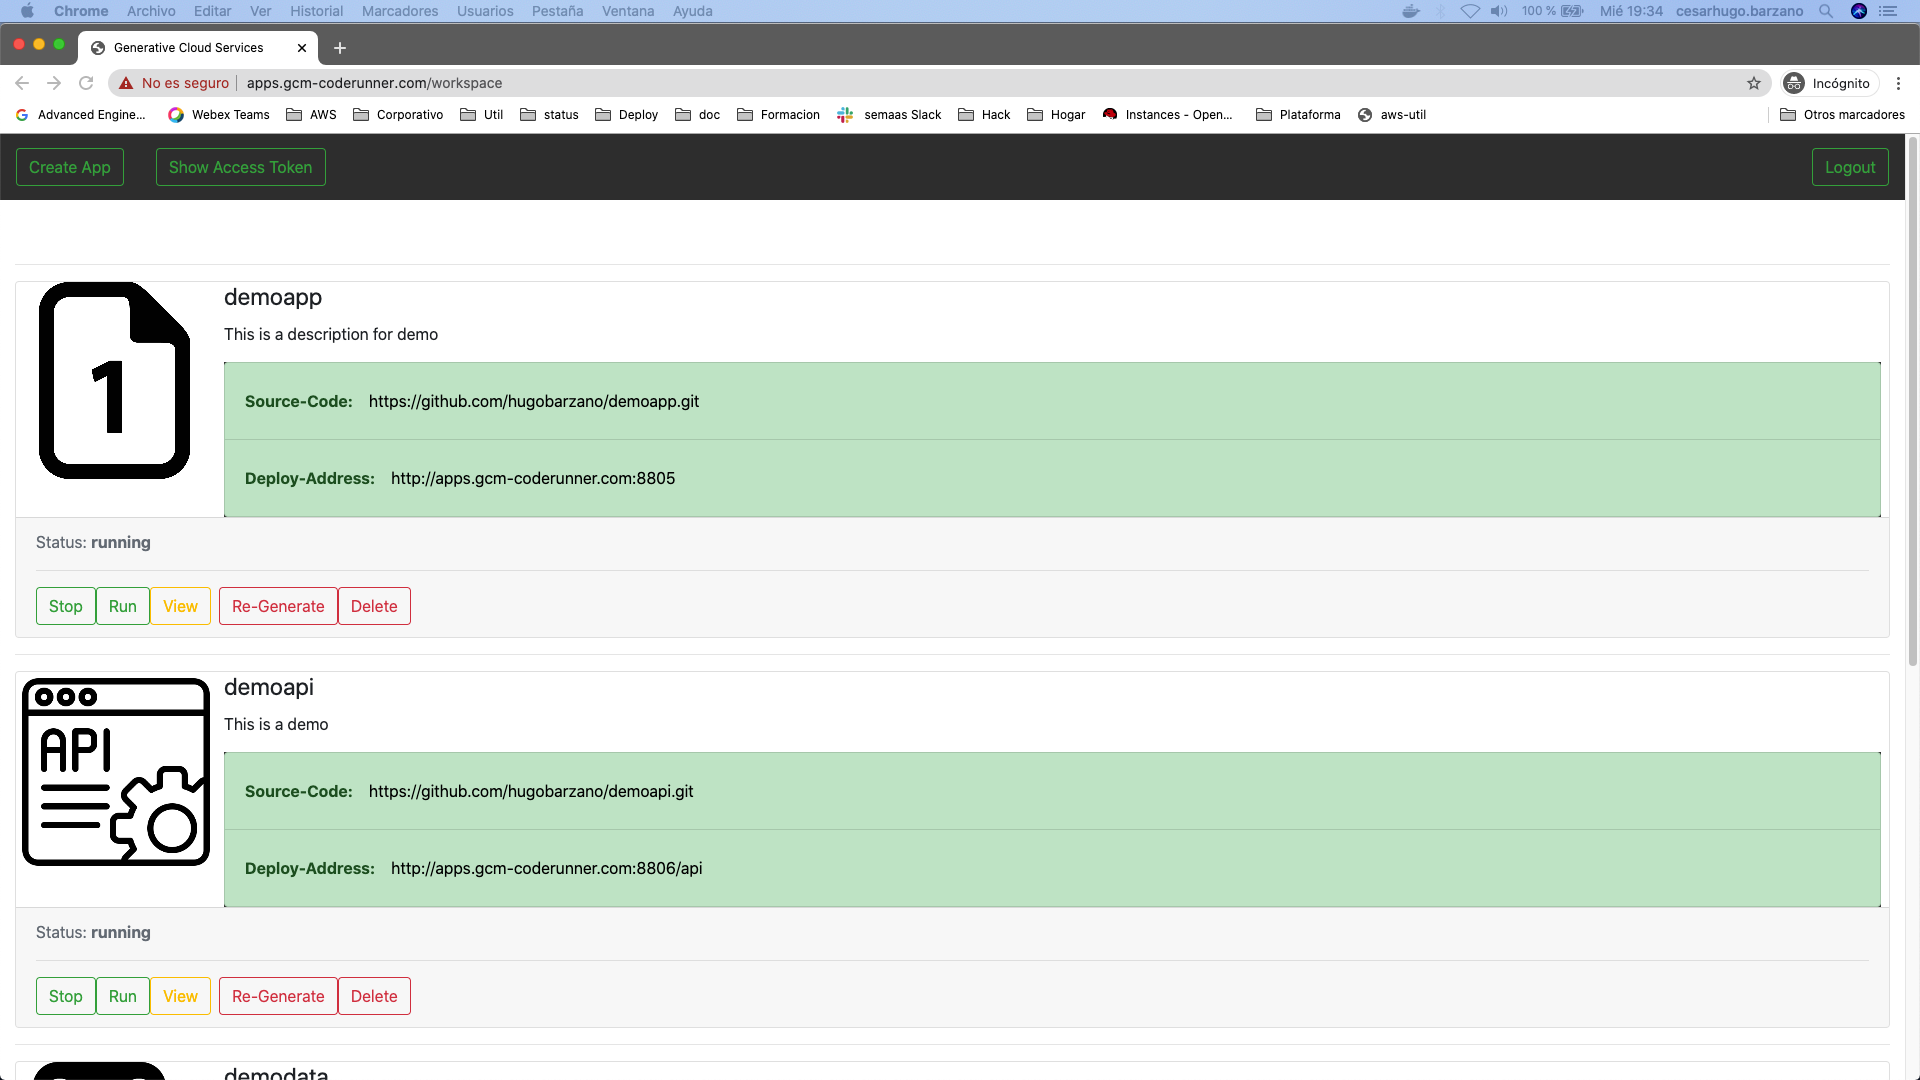
\includegraphics[scale=0.2]{imagenes/casouso/1_1.png}
\caption{  Generando Aplicaciones:Workspace I  }
\end{figure}


\begin{figure}[H]
\centering
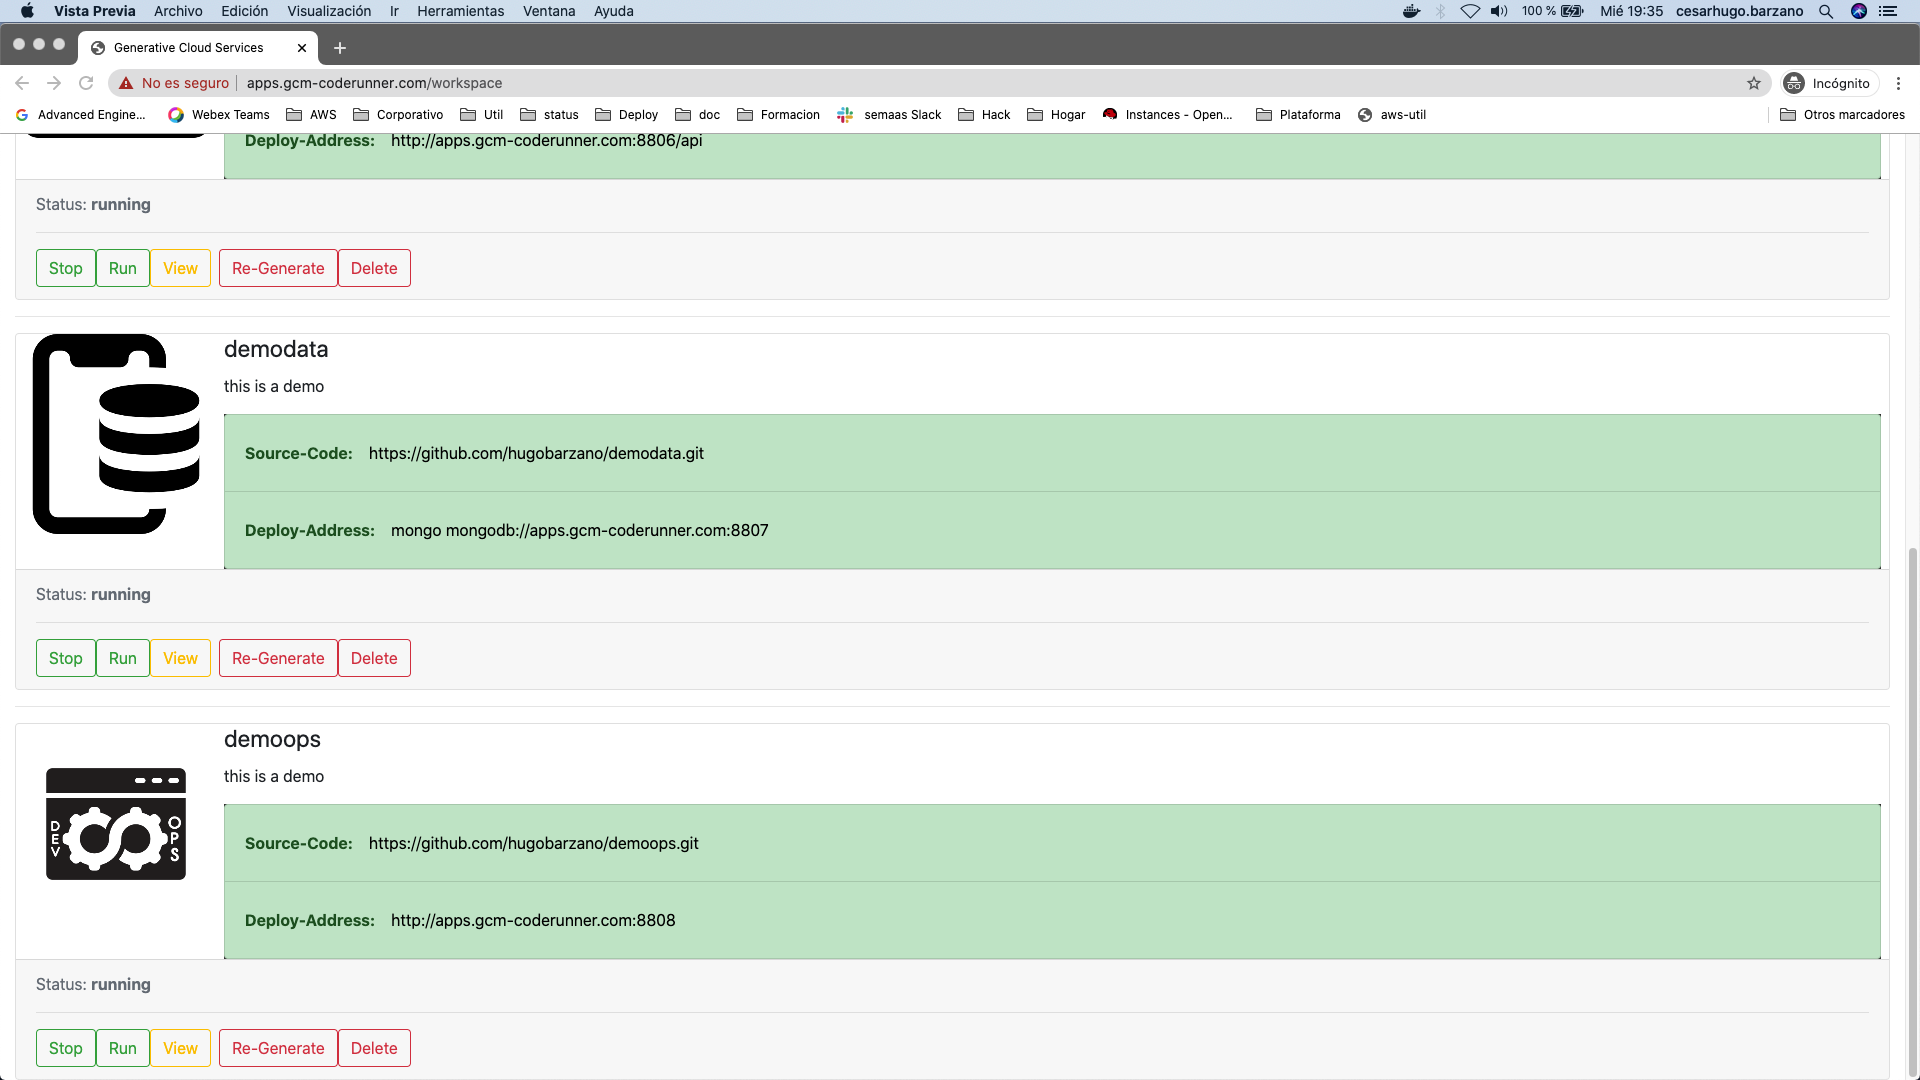
\includegraphics[scale=0.2]{imagenes/casouso/1_2.png}
\caption{   Generando Aplicaciones:Workspace II }
\end{figure}

\subsection{Consumiendo Aplicaciones}

El sistema dota al usuario de las operaciones básicas para consumir las aplicaciones generas. Esta sección ejemplifica como el usuario es capaz de consumir u operar una API-Rest y un servicio de datos. Las operaciones que se muestran a continuación son comunes a todas las aplicaciones producidas por el sistema. 

\subsubsection{Consumiendo Api-Rest}
Para consumir la aplicación generada \textbf{demoapi} el usuario dispone de las siguientes operaciones. Haciendo click en el botón \textbf{Stop} detiene el actual despliegue de la aplicación, liberando los recursos virtuales consumidos por ella y cambiando su estado:

\begin{figure}[H]
\centering
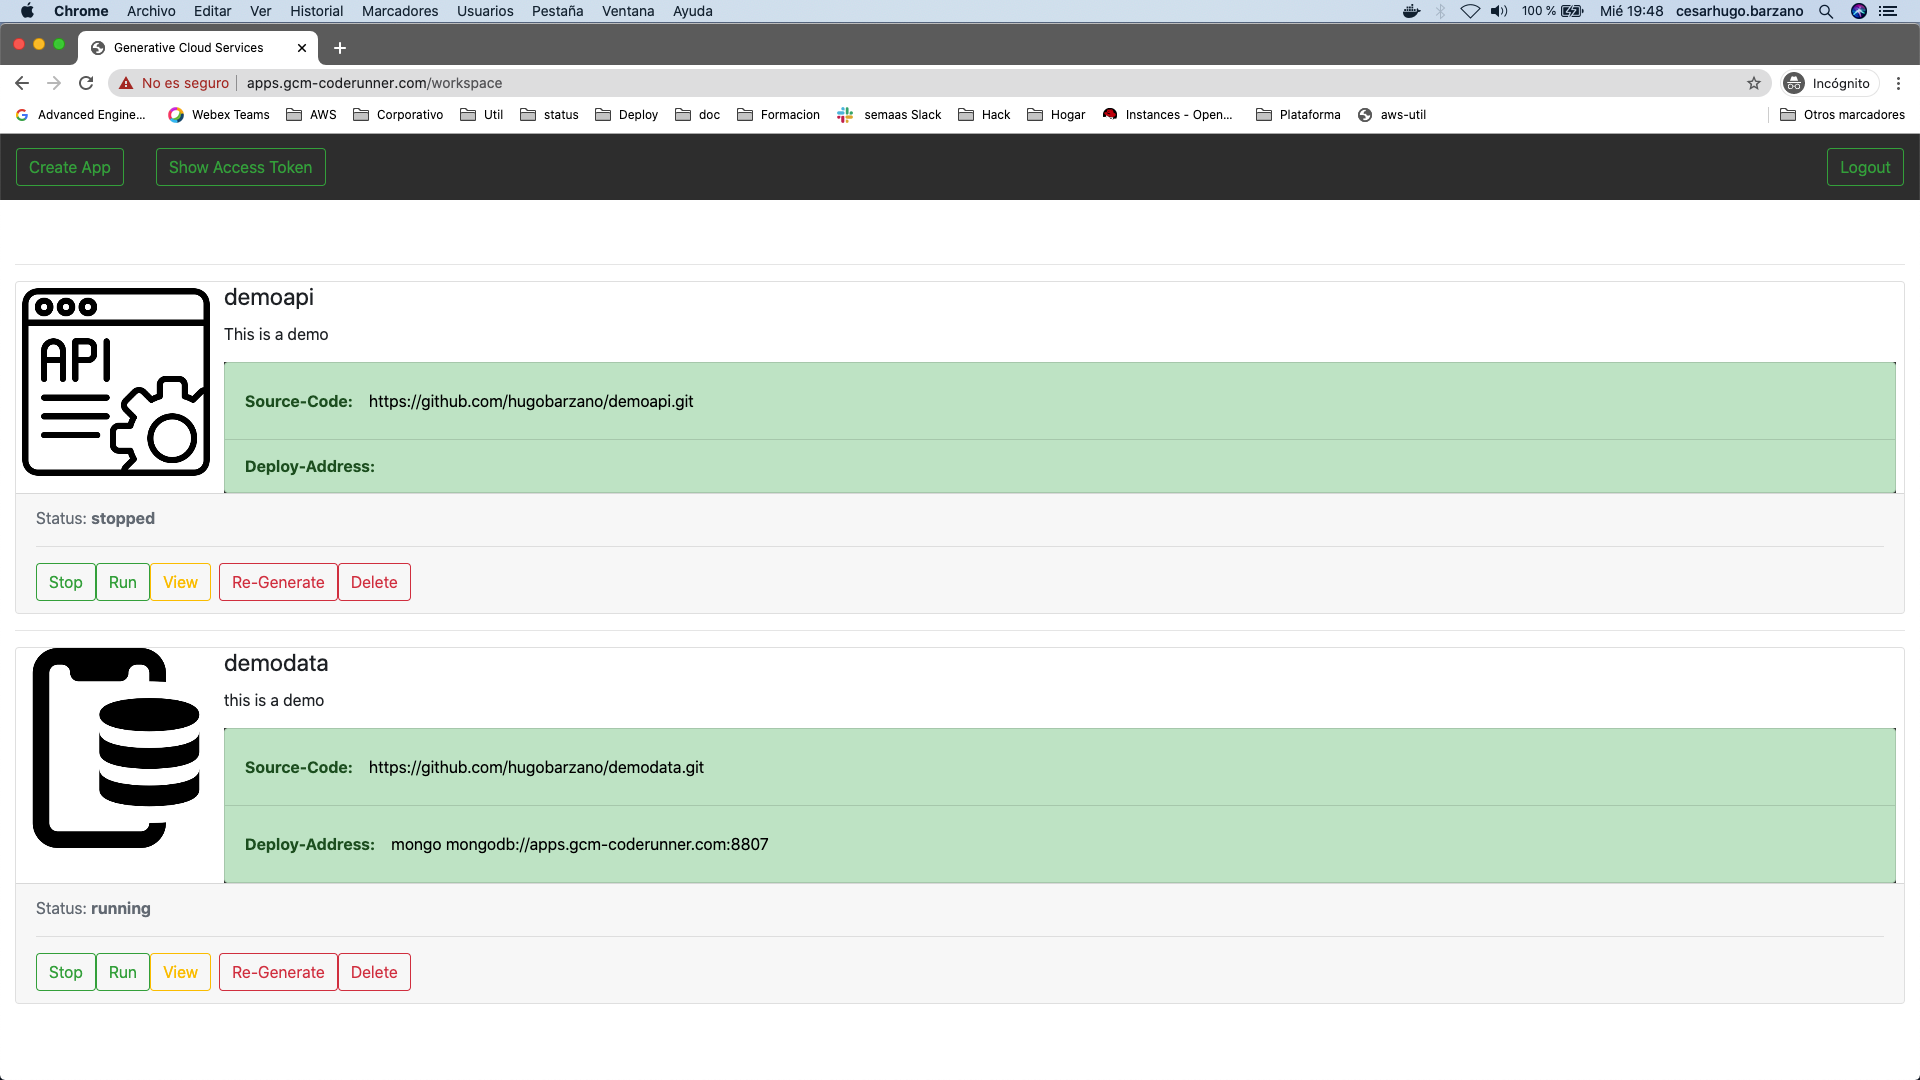
\includegraphics[scale=0.2]{imagenes/casouso/1_3.png}
\caption{  Consumiendo Aplicaciones: Api-Rest  Stop}
\end{figure}

Haciendo click en el botón \textbf{Run} se produce un nuevo despliegue de la aplicación utilizando para ello la última versión generada del artefacto ( la imagen docker) 


\begin{figure}[H]
\centering
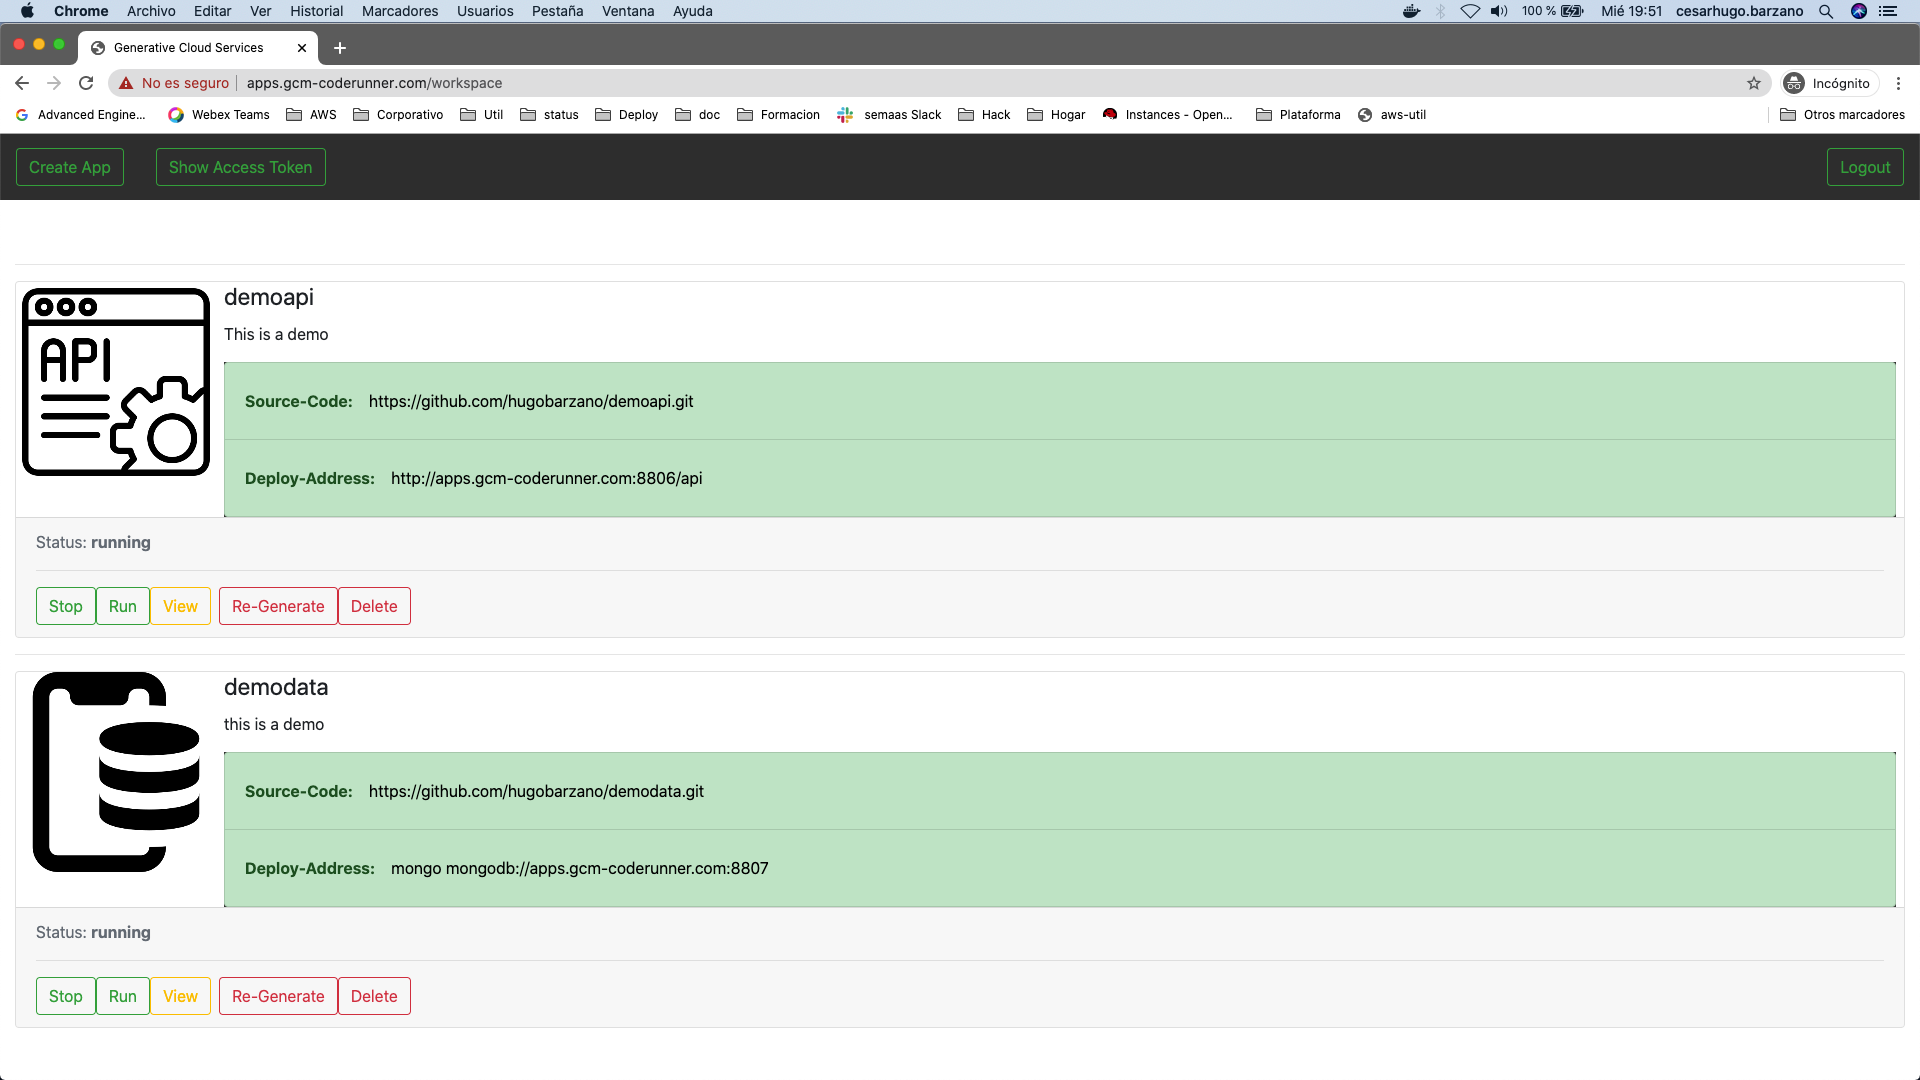
\includegraphics[scale=0.2]{imagenes/casouso/1_4.png}
\caption{ Consumiendo Aplicaciones: Api-Rest Run  }
\end{figure}


Haciendo click en el botón \textbf{View} el usuario es redirigido a una vista concreta de la aplicación. 

\begin{figure}[H]
\centering
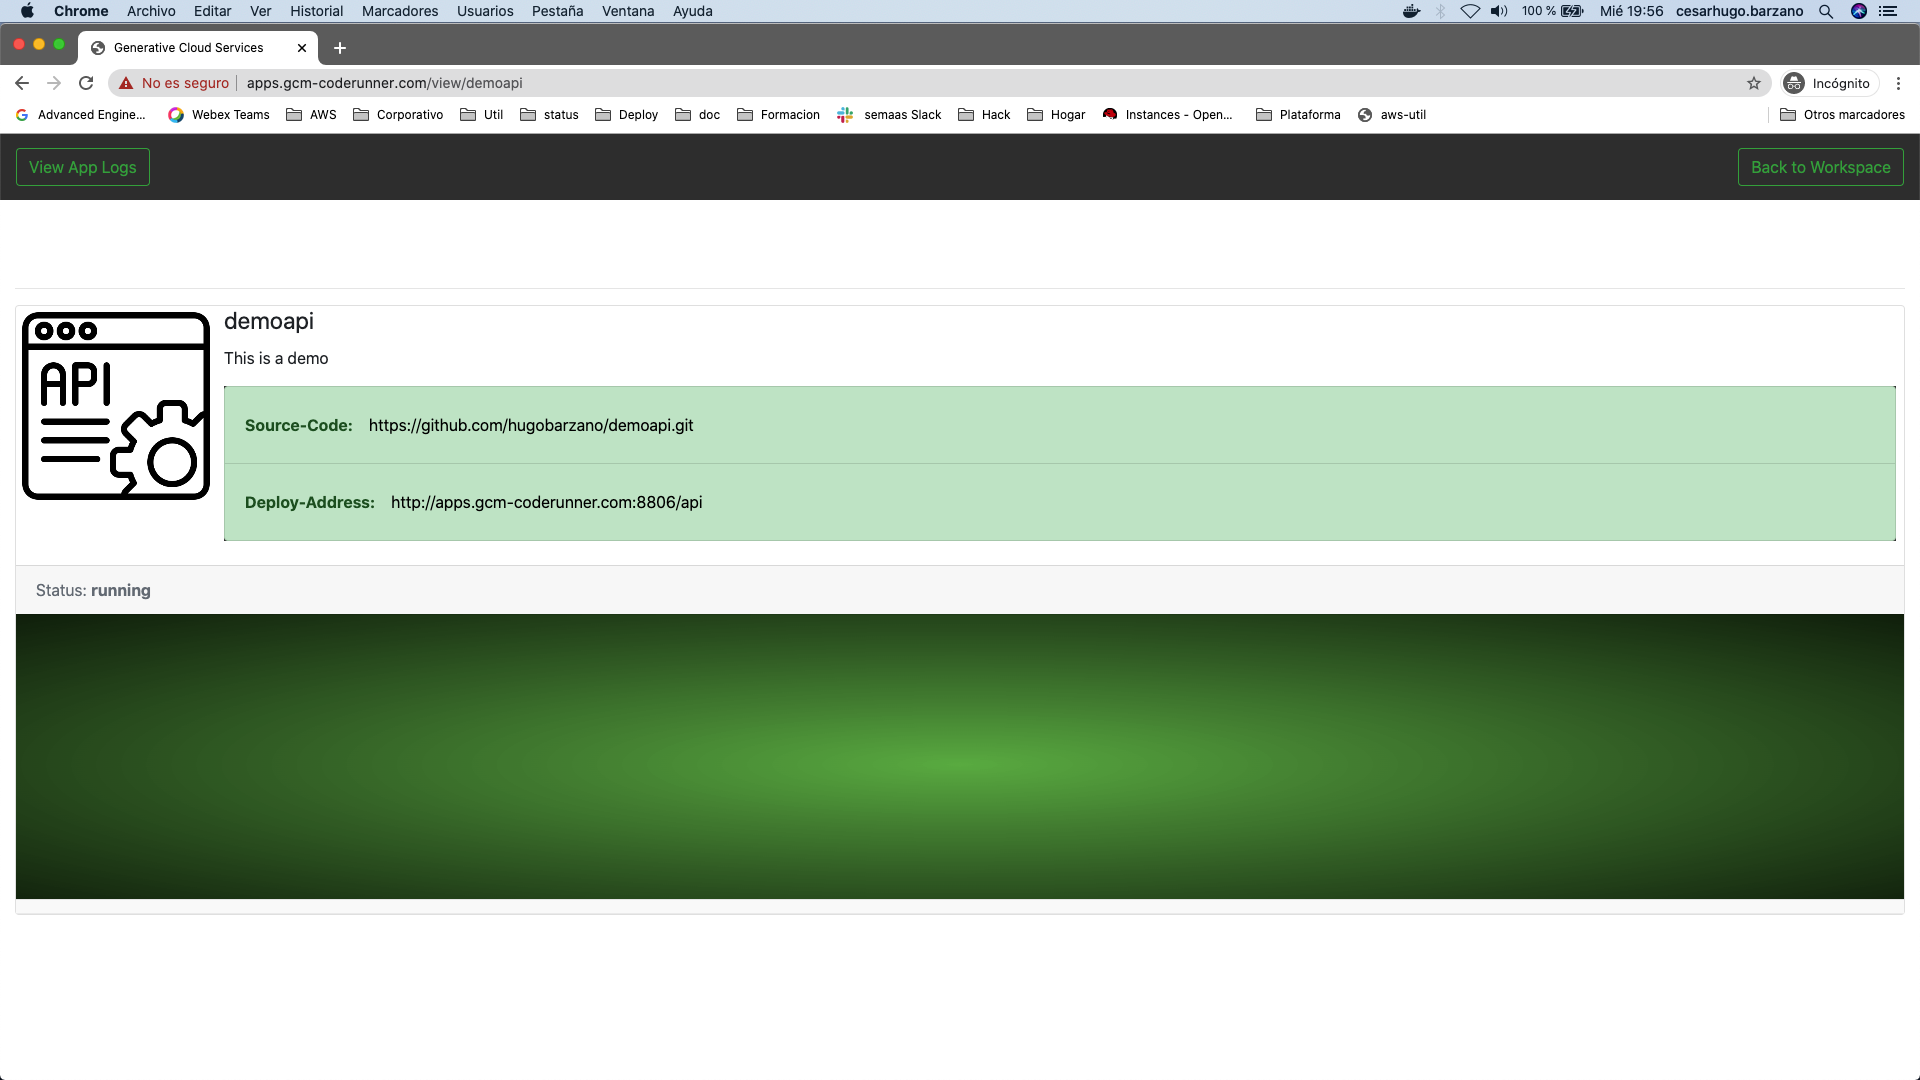
\includegraphics[scale=0.2]{imagenes/casouso/1_5.png}
\caption{ Consumiendo Aplicaciones: Api-Rest View   }
\end{figure}

El sistema permite inspeccionar el trafico atendido por la aplicación en tiempo real haciendo click en el botón \textbf{View App Logs}. Esta operación abre un socket TCP con el docker que ejecuta la aplicación y emite en streaming todos los logs producidos por la misma. Las siguientes evidencias muestran operaciones básicas realizadas utilizando la interfaz de usuario que acompaña a las aplicaciones de naturaleza Api-Rest:

\begin{figure}[H]
\centering
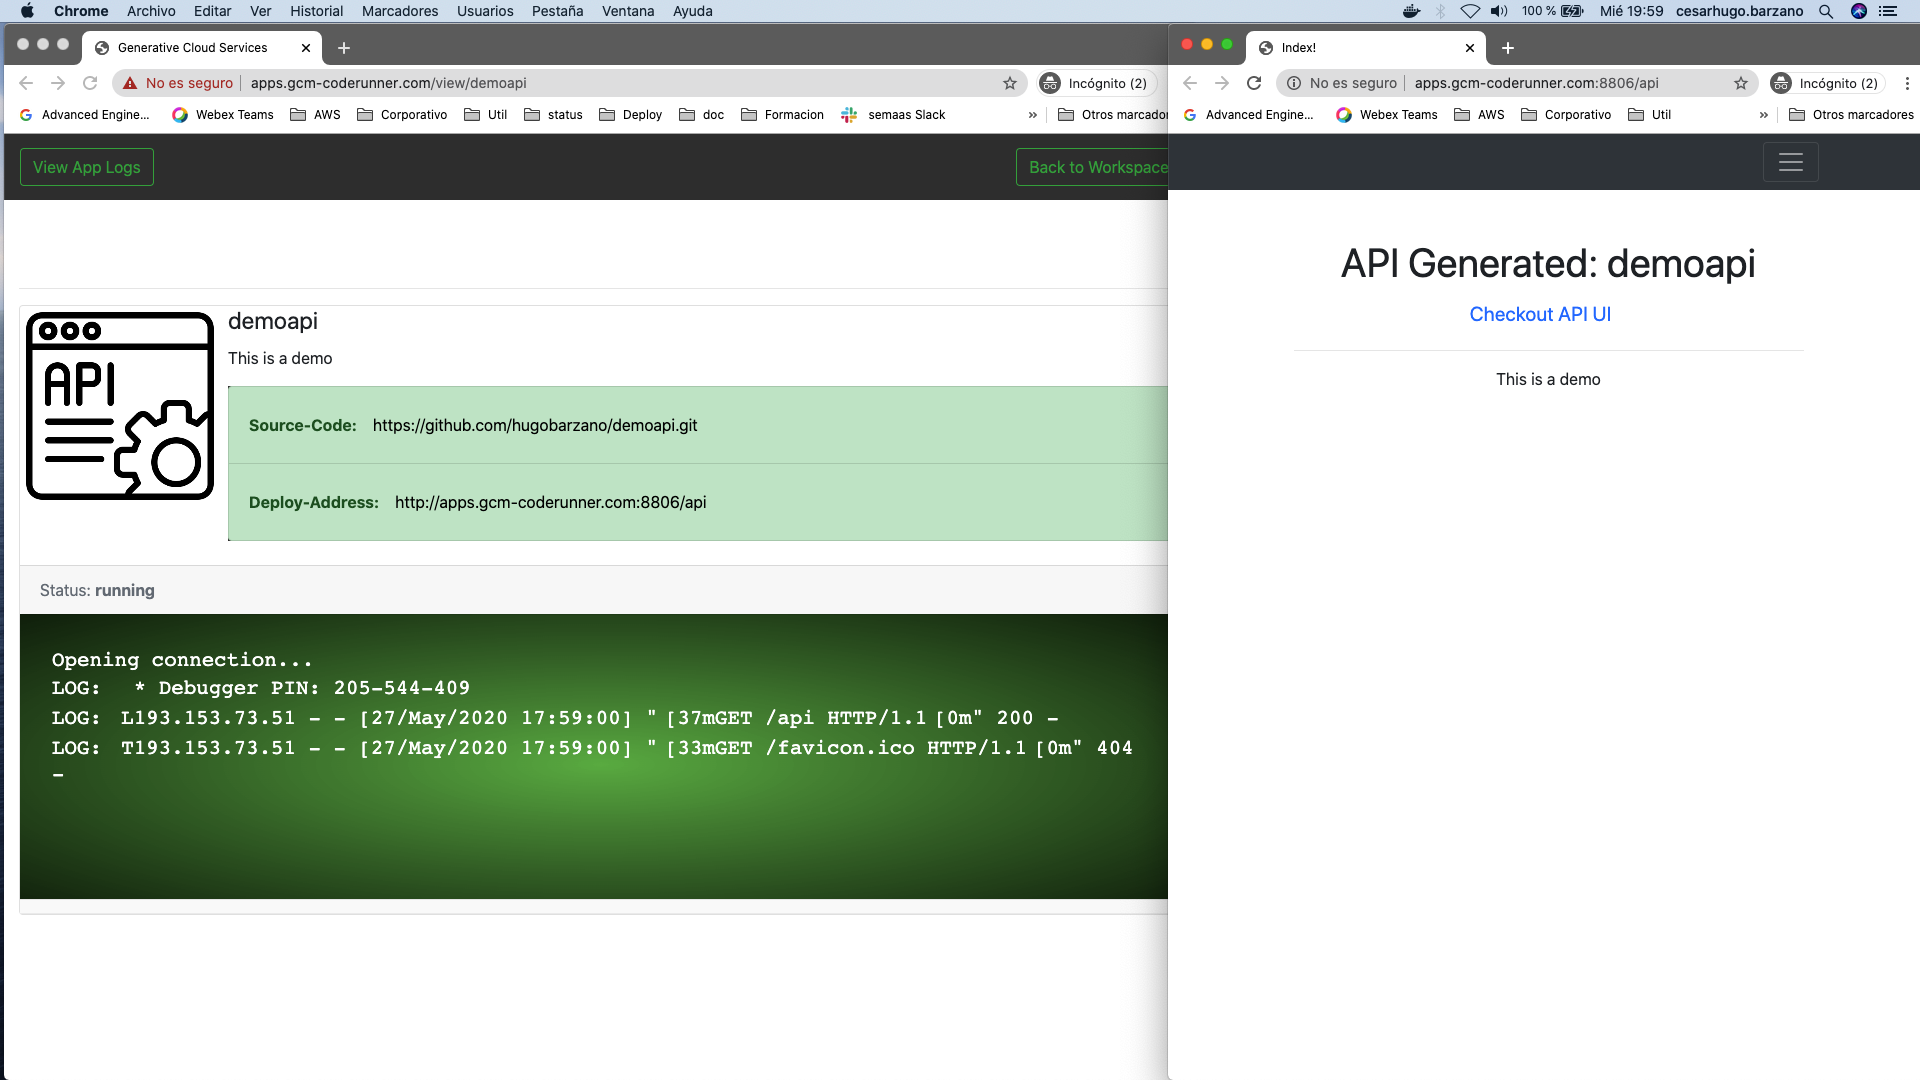
\includegraphics[scale=0.2]{imagenes/casouso/1_7.png}
\caption{  Consumiendo Aplicaciones: Api-Rest View Logs Index }
\end{figure}


\begin{figure}[H]
\centering
\includegraphics[scale=0.2]{imagenes/casouso/1_8.png}
\caption{  Consumiendo Aplicaciones: Api-Rest View Logs UI }
\end{figure}


\begin{figure}[H]
\centering
\includegraphics[scale=0.2]{imagenes/casouso/1_10.png}
\caption{ Consumiendo Aplicaciones: Api-Rest View Logs POST  }
\end{figure}

\begin{figure}[H]
\centering
\includegraphics[scale=0.2]{imagenes/casouso/1_11.png}
\caption{ Consumiendo Aplicaciones: Api-Rest View Logs DELETE  }
\end{figure}

\subsubsection{Consumiendo Data-Service}

Continuando con el caso de uso de como consumir las aplicaciones generadas se presenta un servicio de datos. En este ejemplo el usuario inspecciona una base de datos MongoDB: 

\begin{figure}[H]
\centering
\includegraphics[scale=0.2]{imagenes/casouso/1_13.png}
\caption{ Consumiendo Aplicaciones: Data-Service View Logs  }
\end{figure}

En este caso de uso, es necesario un cliente por linea de comandos para este tipo de base de datos haciendo uso de la terminal de un sistema operativo, los logs de la aplicación registran el numero de nuevas conexiones: 

\begin{figure}[H]
\centering
\includegraphics[scale=0.2]{imagenes/casouso/1_14.png}
\caption{  Consumiendo Aplicaciones: Data-Service View Logs Conexiones !  }
\end{figure}

\begin{figure}[H]
\centering
\includegraphics[scale=0.2]{imagenes/casouso/1_15.png}
\caption{  Consumiendo Aplicaciones: Data-Service View Logs Conexiones !I  }
\end{figure}

\begin{figure}[H]
\centering
\includegraphics[scale=0.2]{imagenes/casouso/1_16.png}
\caption{ Consumiendo Aplicaciones: Data-Service View Logs Conexiones !II   }
\end{figure}

\begin{figure}[H]
\centering
\includegraphics[scale=0.2]{imagenes/casouso/1_17.png}
\caption{ Consumiendo Aplicaciones: Data-Service View Logs Conexiones !V   }
\end{figure}



\subsection{Actualizando Aplicaciones}

El sistema proporciona al usuario los mecanismos necesarios para evolucionar las aplicaciones generas, de esta forma permite que el usuario manipule, pruebe, mejore y aprenda utilizando el código generado. En última instancia el usuario es capaz de re-generar la aplicación devolviéndola a su estado inicial. El sistema presenta los siguientes mecanismos:

\subsubsection{Flujo Continuo de Integración Software}

El primer mecanismo integrado en todas las aplicaciones es el flujo de integración y entrega continuos que permiten al usuario integrar nuevas funcionalidades siguiendo buenas prácticas, para ello, dada una aplicación Single-Page en ejecución:

\begin{figure}[H]
\centering
\includegraphics[scale=0.2]{imagenes/casouso/2_1.png}
\caption{ Actualizando Aplicaciones: Single-Page en Ejecución  }
\end{figure}

\begin{figure}[H]
\centering
\includegraphics[scale=0.2]{imagenes/casouso/2_2.png}
\caption{  Actualizando Aplicaciones: Single-Page Consulta }
\end{figure}

 El usuario ha de clonar la aplicación en su sistema local, haciendo uso de la url del repositorio proporcionada:
 
 \begin{figure}[H]
\centering
\includegraphics[scale=0.2]{imagenes/casouso/2_3.png}
\caption{  Actualizando Aplicaciones: Single-Page Clonar I }
\end{figure}


\begin{figure}[H]
\centering
\includegraphics[scale=0.2]{imagenes/casouso/2_4.png}
\caption{  Actualizando Aplicaciones: Single-Page Clonar II }
\end{figure}

\begin{lstlisting}[language=json,firstnumber=1]
git clone https://github.com/hugobarzano/demoapp.git
cd demoapp
atom . #editor de texto
\end{lstlisting}

 Ha de integrar nueva funcionalidad, en el caso de está aplicación, modificar el color de la hoja de estilos css:
 
 \begin{figure}[H]
\centering
\includegraphics[scale=0.2]{imagenes/casouso/2_5.png}
\caption{ Actualizando Aplicaciones: Single-Page CSS   }
\end{figure}

 Subir los cambios a la rama Master del repositorio:
 
 
\begin{lstlisting}[language=json,firstnumber=1]
git add .
git commit -a -m "ADD push changes demo"
git push
\end{lstlisting}


 
 El flujo de integración continua se dispara ante el evento \textbf{push} relacionado con subir nuevo código al repositorio y de nuevo somete a la aplicación a las mismas etapas que cuando fue generada:
 
  \begin{figure}[H]
\centering
\includegraphics[scale=0.2]{imagenes/casouso/2_6.png}
\caption{  Actualizando Aplicaciones: Single-Page CI Start }
\end{figure}

  \begin{figure}[H]
\centering
\includegraphics[scale=0.2]{imagenes/casouso/2_7.png}
\caption{ Actualizando Aplicaciones: Single-Page CI Finish  }
\end{figure}

 Una vez completado el ciclo de integración continua el usuario percibe que una nueva Release y un nuevo Arterfacto están disponibles en el repositorio:
 
   \begin{figure}[H]
\centering
\includegraphics[scale=0.2]{imagenes/casouso/2_8.png}
\caption{  Actualizando Aplicaciones: Single-Page Release 0.0.1  }
\end{figure}

  \begin{figure}[H]
\centering
\includegraphics[scale=0.2]{imagenes/casouso/2_9.png}
\caption{  Actualizando Aplicaciones: Single-Page Artefecto 0.0.1 }
\end{figure}
 
 El usuario ha de poner el foco en su \textbf{Workspace} , hacer clic en el botón \textbf{Stop} y de nuevo en el botón \textbf{Run}, desplegando así la nueva versión de la aplicación. 
 
   \begin{figure}[H]
\centering
\includegraphics[scale=0.2]{imagenes/casouso/2_10.png}
\caption{   Actualizando Aplicaciones: Single-Page Stop 0.0.0  }
\end{figure}
 
 
   \begin{figure}[H]
\centering
\includegraphics[scale=0.2]{imagenes/casouso/2_11.png}
\caption{   Actualizando Aplicaciones: Single-Page Run 0.0.1  }
\end{figure}
 
 Si ahora vuelve a consumir la aplicación en la dirección de despliegue proporcionada, percibe que el cambio ha sido aplicado y desplegado. 
 
 
   \begin{figure}[H]
\centering
\includegraphics[scale=0.2]{imagenes/casouso/2_12.png}
\caption{  Actualizando Aplicaciones: Single-Page Consulta 0.0.1 }
\end{figure}

\subsubsection{Trabajo Local}

El sistema produce las herramientas necesarias para trabajar en local con las aplicaciones. Para poder interactuar con el repositorio de código y realizar operaciones no públicas, como por ejemplo compilar y subir una nueva versión sin seguir el ciclo de integración software es necesario utilizar el token de acceso del usuario. Con su foco en el \textbf{Workspace}, el usuario ha de hacer click en el botón \textbf{Show Access Token}

   \begin{figure}[H]
\centering
\includegraphics[scale=0.2]{imagenes/casouso/3_1.png}
\caption{  Trabajo Local:  Show Access Token}
\end{figure}

   \begin{figure}[H]
\centering
\includegraphics[scale=0.2]{imagenes/casouso/3_3.png}
\caption{ Trabajo Local:  Access Token  }
\end{figure}

La idea es que el sistema ilustre al usuario en como ha de trabajar con las aplicaciones generadas, por lo  que haciendo click en el botón \textbf{Help!} el usuario dispone de una guía con las operaciones que puede realizar localmente sobre la aplicación:

   \begin{figure}[H]
\centering
\includegraphics[scale=0.2]{imagenes/casouso/3_4.png}
\caption{   Trabajo Local: Help}
\end{figure}

Por ejemplo, si el usuario integra una nueva funcionalidad sobre la aplicación actual ( 0.0.1) como es el cambio de rojo a azul en la hoja de estilos, puede producir y desplegar una nueva versión sin ejecutar el ciclo de integración continua

   \begin{figure}[H]
\centering
\includegraphics[scale=0.2]{imagenes/casouso/3_5.png}
\caption{   Trabajo Local: Single-Page Actualización CSS}
\end{figure}

   \begin{figure}[H]
\centering
\includegraphics[scale=0.2]{imagenes/casouso/3_6.png}
\caption{ Trabajo Local: Single-Page make push  }
\end{figure}

De esta forma, se crean una nueva Release y un nuevo artefacto 

   \begin{figure}[H]
\centering
\includegraphics[scale=0.2]{imagenes/casouso/3_7.png}
\caption{  Trabajo Local: Single-Page Release 0.0.2 }
\end{figure}

   \begin{figure}[H]
\centering
\includegraphics[scale=0.2]{imagenes/casouso/3_8.png}
\caption{ Trabajo Local: Single-Page Artefacto 0.0.2  }
\end{figure}


 El usuario ha de poner el foco en su \textbf{Workspace} , hacer clic en el botón \textbf{Stop} y de nuevo en el botón \textbf{Run}, desplegando así la nueva versión de la aplicación. 
 
\begin{figure}[H]
\centering
\includegraphics[scale=0.2]{imagenes/casouso/3_9.png}
\caption{ Trabajo Local: Single-Page Stop 0.0.1    }
\end{figure}
 
 
   \begin{figure}[H]
\centering
\includegraphics[scale=0.2]{imagenes/casouso/3_10.png}
\caption{  Trabajo Local: Single-Page Run 0.0.2 }
\end{figure}
 
 Si ahora vuelve a consumir la aplicación en la dirección de despliegue proporcionada, percibe que el cambio local ha sido aplicado y desplegado en forma de nueva versión
 
 
   \begin{figure}[H]
\centering
\includegraphics[scale=0.2]{imagenes/casouso/3_11.png}
\caption{   Trabajo Local: Single-Page Consulta 0.0.2}
\end{figure}


\subsubsection{Re-Generación}

Si por algún motivo, el usuario decide que quiere volver al punto de partida, el sistema proporciona la posibilidad de re-generar la aplicación en cuestión llevando el código fuente modificado a su estado base inicial. Para ello, con el foco en su \textbf{Workspace}, el usuario puede hacer click en el botón \textbf{Re-Generate}

   \begin{figure}[H]
\centering
\includegraphics[scale=0.2]{imagenes/casouso/4_1.png}
\caption{  Re-Generación: Single-Page 0.0.2 }
\end{figure}


   \begin{figure}[H]
\centering
\includegraphics[scale=0.2]{imagenes/casouso/4_2.png}
\caption{  Re-Generación: Single-Page 0.0.2 Stop}
\end{figure}


   \begin{figure}[H]
\centering
\includegraphics[scale=0.2]{imagenes/casouso/4_3.png}
\caption{ Re-Generación: Single-Page Generating  }
\end{figure}


   \begin{figure}[H]
\centering
\includegraphics[scale=0.2]{imagenes/casouso/4_4.png}
\caption{  Re-Generación: Single-Page Building }
\end{figure}


   \begin{figure}[H]
\centering
\includegraphics[scale=0.2]{imagenes/casouso/4_5.png}
\caption{  Re-Generación: Single-Page Ready }
\end{figure}


   \begin{figure}[H]
\centering
\includegraphics[scale=0.2]{imagenes/casouso/4_6.png}
\caption{  Re-Generación: Single-Page Release 0.0.3 }
\end{figure}


   \begin{figure}[H]
\centering
\includegraphics[scale=0.2]{imagenes/casouso/4_7.png}
\caption{  Re-Generación: Single-Page Artefacto 0.0.3 }
\end{figure}


   \begin{figure}[H]
\centering
\includegraphics[scale=0.2]{imagenes/casouso/4_8.png}
\caption{  Re-Generación: Single-Page 0.0.3 Running }
\end{figure}


   \begin{figure}[H]
\centering
\includegraphics[scale=0.2]{imagenes/casouso/4_9.png}
\caption{ Re-Generación: Single-Page 0.0.3 Consulta  }
\end{figure}

\subsubsection{Limpieza}

Si el usuario considera finalizado su trabajo puede eliminar todos los recursos virtuales creados por el sistema haciendo click en el botón \textbf{Delete}


   \begin{figure}[H]
\centering
\includegraphics[scale=0.2]{imagenes/casouso/5_1.png}
\caption{  Limpieza: Single-Page 0.0.3 Delete }
\end{figure}

La aplicación entra en estado de no retorno \textbf{deleting} y se procede  a la limpieza de los recursos virtuales utilizados. 

   \begin{figure}[H]
\centering
\includegraphics[scale=0.2]{imagenes/casouso/5_2.png}
\caption{  Limpieza: Single-Page 0.0.3 Deleting }
\end{figure}

   \begin{figure}[H]
\centering
\includegraphics[scale=0.2]{imagenes/casouso/5_3.png}
\caption{ Limpieza: Workspace  }
\end{figure}


\chapter{Conclusiones}

Se ha demostrado como el uso de servicios cloud y la programación generativa son capaces de producir un sistema generativo que ofrece al usuario final un entorno virtual capaz de interpretar especificaciones de aplicación, generar su código fuente y crear los recursos necesarios para que sean consumidas por Internet.   Este proyecto pone de manifiesto que la integración de buenas practicas en los procesos relativos al ciclo de vida del desarrollo software mejora aspectos tales como la rápida iteración e integración  de nuevas funcionalidades. Por otra parte también se beneficia la entrega constante de nuevas versiones facilitando la evolución del software junto con mejoras en el tiempo de implantación fruto del despliegue continuo. El proporcionar un sistema cloud como este favorece el aprendizaje a los desarrolladores ya que disponen de un conjunto de aplicaciones de prueba en cuestión de segundos.  

 El proceso de desarrollo software mejora integrando buenas prácticas y automatizando las tareas recurrentes, la gran barrera a superar viene impuesta normalmente por los actuales procesos de las organizaciones ya que actualizar su modelo de trabajo conlleva la inversión de una gran cantidad de recursos ( económicos y humanos).

\section{Mejoras y Trabajos Futuros}

En esta sección se presentan ciertas mejoras a integrar en el proyecto mejorando sus aspectos principales y dando paso a futuras ramas de estudio. 

\subsection{Proceso Generativo}

Actualmente el motor de plantillas encargado de generar las aplicaciones está completamente integrado en el código fuente de Code-Runner. Se propone como mejora la externalización de dichas plantillas a un repositorio de código ajeno al proyecto. De esta manera se podría trabajar en nuevas versiones de las aplicaciones generadas sin necesidad de liberar y desplegar una nueva versión del sistema software en si. Como punto de partida para la mejora se propone por ejemplo que Code-Runner sea capaz de cargar en memoria el contenido del repositorio de plantillas y utilizar dicho contenido para la producción de código. Adicionalmente este mecanismo debería refrescar periódicamente la copia en memoria del repositorio, de esta forma el sistema sería capaz de integrar nuevas versiones a generar sin perdida de servicio. 
\subsubsection{Especificación de Aplicación}

Se propone como mejora adicional la actualización del la especificación de aplicación solicitada al usuario para cubrir escenarios mas complejos, como por ejemplo para la  generación de aplicaciones  Api-Rest podrían definirse diversos modelos de datos junto con las relaciones u operaciones que existan entre ellos. Los servicios de datos también puede mejorar si la especificación soportara configuración de credenciales(contraseñas).

\subsubsection{Importar Aplicaciones}

Se propone como mejora la capacidad de importar aplicaciones ya existentes en repositorios del usuario. La idea es la de inferir desde el repositorio de código lo necesario para categorizar la aplicación y  poder generar los elementos software (configuración, scripts, código fuente, documentación) necesarios para que la aplicación forme parte del ecosistema de Code-Runner.  

\subsection{Naturaleza y Tecnología}

Se ha demostrado que el  uso de Docker como motor de virtualización ligera permite generalizar el despliegue y operación de aplicaciones de distinta naturaleza y de distinta tecnología. Se propone como mejora categorizar nuevas naturalezas de aplicación así como integrar aplicaciones basadas en otras tecnologías. Para ello se presenta como referencia el conjunto de imágenes docker disponibles públicamente en Docker Hub:\cite{dhub}   \url{https://hub.docker.com/search?q=&type=image}

\subsubsection{Definir el Concepto Proyecto Generativo}

La idea sería definir un nuevo modelo de datos definido proyecto generativo con idea de representar a un conjunto reducido de aplicaciones de diversa naturaleza y tecnología que funcionan en conjunto para formar una solución generativa. Por ejemplo generar una Api-Rest y su servicio de persistencia como una sola entidad que engloba ambas aplicaciones. Para modelarlo se propone hacer uso de orquestadores de contenedores como Kubernetes\cite{kube} o Docker-Compose\url{https://docs.docker.com/compose}.  

\subsection{Testing}

 En el proceso de desarrollo software, el testing o validación es una etapa fundamental para garantizar el correcto funcionamiento de las piezas desarrolladas así como la integración de nuevas funcionalidades. Aunque en el ciclo de integración continua definido para las aplicaciones generadas por el sistema se contempla una etapa de ejecución de pruebas unitarias no se están generando el código fuente necesario para materializarlas. Por ello, se propone como trabajo futuro la definición y generación de pruebas software para las aplicaciones generadas en función de su naturaleza. Las pruebas pueden ser en primer lugar de carácter unitario para ser ejecutadas durante el ciclo de integración continua y en segundo lugar de carácter sistema o pruebas de caja negra para ser ejecutadas cada vez que se despliega una nueva versión. 

\subsection{Material Didáctico}

Con el objetivo de mejorar el aprendizaje del usuario en el desarrollo, uso y consumo de aplicaciones web o servicios cloud se propone como trabajo futuro la definición de material didáctico, documentación exhaustiva, ejemplos y retos que acompañen al código fuente generado. De esta forma, el sistema proporcionaría al usuario de una linea de trabajo o actividades a realizar con el software que ha decidido generar, enriqueciendo y facilitando su proceso de aprendizaje. 

\subsection{Interfaz de Sistema Cloud}


El estado actual del Code-Runner produce aplicaciones consumibles tal que  \textbf{ https://code-runner.com:8081/api/}  donde probar la solución generada. Es decir: 

   \begin{figure}[H]
\centering
\includegraphics[scale=0.5]{imagenes/api.png}
\caption{ Ejemplo App  }
\end{figure}
La extensión que se propone sería la de incluir, en la etapa de generación de código, todo lo necesario para servir una interfaz interna o de sistema de manera común a todas las soluciones generadas, sirviendo  cierta información sobre la aplicación:


   \begin{figure}[H]
\centering
\includegraphics[scale=0.5]{imagenes/system.png}
\caption{ Ejemplo Interfaz Sistema  }
\end{figure}

la interfaz \textbf{\char`_system/} podría servir información como por ejemplo:

\begin{enumerate}
\item\textbf{ https://code-runner.com:8081/\char`_system/version }: Versión software
\item \textbf{https://code-runner.com:8081/\char`_system/config }: Configuración de la Aplicación
\item \textbf{https://code-runner.com:8081/\char`_system/metrics }: Métricas 
\end{enumerate}

La idea es aprovechar en la medida de lo posible esta interfaz para obtener información de las soluciones generadas y servir esta información desde la interfaz de usuario de Code-Runner junto con las obtenidas del contenedor donde se está ejecutando. Incluso las aplicaciones con esta interfaz podrían consumir recursos comunes al dominio cloud, mostrando un comportamiento de plataforma o de sistema cloud. 

\chapter{ Anexo}

\section{Ficheros de Ejemplo}

\subsubsection{Modelo de Datos:  Aplicación}\label{anexmodel}


\begin{lstlisting}[language=json,firstnumber=1]
{
    "_id" : "example",
    "repo" : "https://github.com/hugobarzano/example.git",
    "spec" : {
        "tech" : "python",
        "modelJson" : "                        {\"active\":true, \"name\":\"thing name\", \"value\":33}\r\n                    ",
        "dockerId" : "aeccdfea4cf6f0bc0ede31977edc791ed87e0e467b1dfd9222005e63feff8598",
        "port" : "8083",
        "nature" : "Api-Rest"
    },
    "des" : "this is a description",
    "url" : "http://35.233.23.148:8083/api",
    "owner" : "hugobarzano",
    "status" : "running"
}
\end{lstlisting}

\subsubsection{Flujo de Integración Continua}\label{anexci}

\begin{lstlisting}[language=json,firstnumber=1]
name: Continuous Integration Workflow
on:
  push:
    branches:
      - master
jobs:
  test:
    runs-on: ubuntu-latest
    steps:
      - uses: actions/checkout@v1
      - name: Run tests
        run: |
          make setup
          make test
  push:
    needs: test
    runs-on: ubuntu-latest
    if: github.event_name == 'push'
    steps:
      - uses: actions/checkout@v1
      - name: Build and Push Artifact - Docker Image
        run: |
          make push user=${{ github.actor }} token=${{ secrets.GITHUB_TOKEN }}
\end{lstlisting}

\thispagestyle{empty}

\bibliography{ref/references}
\end{document}
